% !TeX spellcheck = en_GB
%=====================================================================
%	UCT MECHATRONICS GROUP LaTeX THESIS/DISSERTATION TEMPLATE
%---------------------------------------------------------------------
%	Created by:		R.A. Verrinder
%	Date Modified:	Jan 2016
%---------------------------------------------------------------------
%	Compile with:	arara 
%=====================================================================
%	Document properties:
%---------------------------------------------------------------------
%	Paper size:			A4
%	Margins:			1 inch margins (top,bottom,left,right)
%	Printing:			Double sided
%	Base font size:		12pt
%	Line spacing:		
%	Paragraph spacing:	10pt
%	Paragraph indent:	0pt
%=====================================================================

\documentclass[a4paper, 12pt, oneside, openright, parskip=full]{book}

%---------------------------------------------------------------------
%	PACKAGES
%---------------------------------------------------------------------
\usepackage[margin = 1in]{geometry}		
\usepackage{lscape}
\usepackage{rotating}
\usepackage{hyphenat}
\usepackage{setspace}
\usepackage{hyperref}
\usepackage{titlesec}
\usepackage{lastpage}
\usepackage{fancyref}
\usepackage{fancyvrb}
\usepackage{enumitem}

\usepackage{cite}
\usepackage[usenames,dvipsnames]{xcolor}
\usepackage{graphicx}					% Can include graphics
\usepackage{float}						% Can place figures at exact places in text
\usepackage{wrapfig}					% Can wrap text around figures
\usepackage{import}

\usepackage{array}						% Can set column widths in tables
\usepackage{mdframed}					% Can draw boxes around text etc.
\usepackage{subcaption}					% Can place figures side by side
\usepackage{tikz}
\usepackage{pgfplots}
\pgfplotsset{width=10cm,compat=1.9}
%\usepgfplotslibrary{external}
%\tikzexternalize
\usetikzlibrary{arrows.meta}
\usetikzlibrary{positioning}		
\usetikzlibrary{shapes.geometric, arrows} % For block diagrams
\usetikzlibrary{circuits.logic.US} 
\usetikzlibrary{calc}
\usepackage[siunitx]{circuitikz}		% Can draw circuits
\usepackage{tikz-timing}				% Can draw timing diagrams
\usepackage{enumerate}
\usepackage{makecell}

\usepackage{hyperref}
\hypersetup{
    colorlinks=true,
    linkcolor=blue,
    filecolor=magenta,      
    urlcolor=cyan,
}

\urlstyle{same}

\usepackage{xspace}						% For box spaces
\usepackage{caption}					% Captions and subcaptions

\usepackage{fix-cm}						% Can set font size
\usepackage{color}						% Can change font color

\usepackage[scaled=0.9]{helvet}			% Helvetica font scaled \phv
\usepackage{courier}					% Courier font \pcr
%\usepackage[ruled,linesnumbered]{algorithm2e}     %Algorithm2e package
\usepackage{xcolor}
\usepackage[ruled,vlined,linesnumbered,resetcount,algochapter]{algorithm2e}
\newcommand\mycommfont[1]{\footnotesize\ttfamily\textcolor{blue}{#1}}
\SetCommentSty{mycommfont}

%\usepackage{mathptmx}					% Times New Roman font
%\usepackage{cmbright}					% Sans serif font
%\normalfont 							% in case the EC fonts aren't available
%\usepackage[T1]{fontenc}				% Used to switch to type 1 font encoding

\usepackage{amsmath, amsthm, amssymb}
\usepackage{datetime}					% Can use dates and times
\usepackage{gensymb}				
\usepackage{multirow}
\usepackage{longtable}
\usepackage{adjustbox}
\usepackage{hhline}
\usepackage{verbatim}

\usepackage{listings}
\usepackage{xcolor}
\usepackage{wasysym}
\usepackage{pifont}
\usepackage{booktabs}
\usepackage{paralist}

%New colors defined below
\definecolor{codegreen}{rgb}{0,0.6,0}
\definecolor{codegray}{rgb}{0.5,0.5,0.5}
\definecolor{codepurple}{rgb}{0.58,0,0.82}
\definecolor{backcolour}{rgb}{0.95,0.95,0.92}

%Code listing style named "mystyle"
\lstdefinestyle{mystyle}{
  backgroundcolor=\color{backcolour},   commentstyle=\color{codegreen},
  keywordstyle=\color{magenta},
  numberstyle=\tiny\color{codegray},
  stringstyle=\color{codepurple},
  basicstyle=\ttfamily\footnotesize,
  breakatwhitespace=false,         
  breaklines=true,                 
  captionpos=b,                    
  keepspaces=true,                 
  numbers=left,                    
  numbersep=5pt,                  
  showspaces=false,                
  showstringspaces=false,
  showtabs=false,                  
  tabsize=2
}

%"mystyle" code listing set
\lstset{style=mystyle}

%confusion matrix
\newcommand\MyBox[2]{
  \fbox{\lower0.75cm
    \vbox to 1.7cm{\vfil
      \hbox to 1.7cm{\hfil\parbox{1.4cm}{#1\\#2}\hfil}
      \vfil}%
  }%
}



%---------------------------------------------------------------------
% 	PAGE FORMATTING
%---------------------------------------------------------------------
% Include page formatting here. 
%---------------------------------------------------------------------
\parskip	= 10pt						% Paragraph spacing
\parindent 	= 0pt						% No para. indent

% Caption margins 80% of text
\captionsetup{width=0.8\textwidth,font=small,labelfont=bf}		

%---------------------------------------------------------------------
%	DOCUMENT PROPERTIES
%---------------------------------------------------------------------
% Fill in your details here. These macro commands can the be used 
% throughout the document. Comment out what is unnecessary.
%---------------------------------------------------------------------
\newcommand{\auth}{Boitumelo Dikoko}								% Author
\newcommand{\titl}{Multiple Mobile Robot SLAM for collaborative mapping and exploration}						% Thesis title
\newcommand{\subtitle}{Subtitle}						% Thesis subtitle
\newcommand{\dept}{Department of Electrical Engineering}% Department 
\newcommand{\uni}{University of Cape Town}				% University
\newcommand{\city}{Rondebosch, Cape Town}				% City
\newcommand{\country}{South Africa}						% Country
\newcommand{\degre}{Master of Science}				% Degree (Doctor of Philosophy 
														% or Master of Science)
\newcommand{\degreeabv}{MSc.}							% Degree abbreviation (PhD or MSc.)			
\newcommand{\aemail}{dkkboi002@myuct.ac.za}			% Author email address
\newcommand{\supervisor}{R.A Verrinder}					% Supervisor
\newcommand{\cosupervisor}{Prof. E. Boje}					% Supervisor
\newcommand{\hod}{Prof. E. Boje}						% Head of Department

\newcommand{\logo}										% UCT Logo
{	
	
\includegraphics[scale = 0.3]{figs/uctLogo}
}

\newdateformat{mydate}{\monthname[\THEMONTH] \THEYEAR} % Month Year date
\newcommand{\key}{Multiple Robot SLAM; Map Merging; Multi-Session Mapping}					   % Keywords (add logical keywords)
\newcommand{\argmin}{\mathop{\mathrm{argmin}}\limits}
\newcommand{\argmax}{\mathop{\mathrm{argmax}}\limits}
%---------------------------------------------------------------------
%	MACROS
%---------------------------------------------------------------------
% Signature box
%---------------------------------------------------------------------
\newcommand*{\signature}[1]
{
	\par\noindent\makebox [5cm]{\hrulefill}
	\par\noindent\makebox [5cm][1]{#1}
}
%---------------------------------------------------------------------
% Macro to select font style
% phv = helvetica (sans serif)
% pcr = courier	  (typewritter font)
%---------------------------------------------------------------------
\def\nfont#1#2
{
	{\fontfamily{#1}\selectfont #2}
}					
%---------------------------------------------------------------------
% NRF statement for those funded by the NRF - comment out if unnecessary
%---------------------------------------------------------------------
\newcommand{\nrf}									   
{	
The financial assistance of the National Research Foundation (NRF) towards this research is hereby acknowledged. Opinions expressed and conclusions arrived at, are those of the author and are not necessarily to be attributed to the NRF.

}
%---------------------------------------------------------------------
% Creates an block for a block diagram
%---------------------------------------------------------------------
\tikzstyle{arrow}=[->,shorten <=1pt,>=stealth',semithick]
%---------------------------------------------------------------------
% Multiplexer
%---------------------------------------------------------------------
\newcommand{\mux}									
{
	\begin{tikzpicture}
		\draw 	(0,0)coordinate  		(O)--++
		 	 	(30:1.5)coordinate 		(A)--++
		  		(90:1.5)coordinate 		(B)--++
		  		(150:1.5)coordinate		(C)--cycle;
		\draw ($(A)!0.5!(B)$)--++(0:1)node[right]{$O$};
		\draw ($(O)!0.5!(A)$)--++(-90:1)--++(180:1.3)node[left]{$S0$};
		\foreach \y/\t in {0.3/0,0.6/1} {
			\draw ($(C)! \y*1 !(O)$)--++(180:1.5) node[left] {$I \t$};}
			\draw (0,1.5) node[right]{$MUX$};
	\end{tikzpicture}
}
%---------------------------------------------------------------------
%block 1
%---------------------------------------------------------------------
\tikzstyle{block}=[rectangle,
				   draw=black,
				   fill=gray!10,
				   thick, 
				   minimum height = 2cm, 
				   text width=0.15*\columnwidth,]
\tikzstyle{input}  		= [coordinate]
\tikzstyle{output} 		= [coordinate]
\tikzstyle{pinstyle} 	= [pin edge={to-,thin,black}]
\tikzstyle{sum} 		= [draw, fill=blue!20, circle, node distance=1cm]
%---------------------------------------------------------------------
%block 2
%---------------------------------------------------------------------
\tikzstyle{block2}=[rectangle,
				   draw=black,
				   fill=gray!10,
				   thick, 
				   minimum height = 1.8cm, 
				   text width=0.1*\columnwidth,]
\tikzstyle{input}  		= [coordinate]
\tikzstyle{output} 		= [coordinate]
\tikzstyle{pinstyle} 	= [pin edge={to-,thin,black}]
\tikzstyle{sum} 		= [draw, fill=blue!20, circle, node distance=1cm]
%---------------------------------------------------------------------
%flow charts
%---------------------------------------------------------------------
\tikzstyle{state}     = 	[rectangle, 
							 text width=0.15*\columnwidth=2cm, 
							 minimum  height=1.5cm, 
							 text centered, 
							 draw=black]
							 
\tikzstyle{statement}  = 	[rectangle, 
							 text width=0.15*\columnwidth=2cm, 
							 minimum  height=0.5cm, 
							 text centered, 
							 draw=black]							 
							 
\tikzstyle{condition}  = 	[rectangle, 
							 text width=0.15*\columnwidth=2cm, 
							 minimum  height=1cm, 
							 rounded corners =10pt,
							 text centered, 
							 draw=black]
\tikzstyle{decision}  = 	[diamond, 
			                 minimum width=2cm, 
			                 minimum height=1cm, 
			                 text centered, 
			                 draw=black]
\tikzstyle{line} = [draw, -latex']


\definecolor{DodgerBlue}{RGB}{30,144,255}

\newcommand{\bluearrow}{\raisebox{0pt}{\tikz{\draw [-Triangle
,DodgerBlue,solid,line width = 1pt](0,0) -- (5.2mm,0);}}}

\newcommand{\redline}{\raisebox{2.5pt}{\tikz{\draw[-,BrickRed,solid,line width = 1pt](0,0) -- (5.2mm,0);}}}

\newcommand{\orangedashed}{\raisebox{2pt}{\tikz{\draw[-,orange,dashed,line width = 1pt](0,0) -- (5.2mm,0);}}}

\newcommand{\robot}{\tikz [baseline=-3pt] \node [shape=isosceles triangle,scale=0.8,draw=black,fill=gray!90,text=black,inner sep=2pt] {};}

\newcommand{\robotest}{\tikz [baseline=-3pt] \node [shape=isosceles triangle,scale=0.8,draw=black,fill=white,text=black,inner sep=2pt] {};}

\newcommand{\landmark}{\tikz [baseline=-3pt] \node [shape=star,star points=7,star point ratio=0.6,scale=1.2,draw=black,fill=gray!90,text=black,inner sep=2pt] {\fontsize{4}{4}\selectfont{$i$}};}

\newcommand{\landmarkest}{\tikz [baseline=-3pt] \node [shape=star,star points=7,star point ratio=0.6,scale=1.1,draw=black,fill=white,text=black,inner sep=2pt] {\fontsize{4}{4}\selectfont{\textcolor{white}{\em{i}}}};}

%=====================================================================
%	Start of the document
%---------------------------------------------------------------------
\begin{document}

%=====================================================================
%	TITLE PAGE
%=====================================================================
\begin{titlepage}
	\centering
	\vspace*{1cm}

%---------------------------------------------------------------------
% Title
%---------------------------------------------------------------------	
	\begin{Huge}					
		\bfseries\titl\par
		\vskip 5mm
		%\hrule
		%\vskip 1.2cm
	\end{Huge}
%---------------------------------------------------------------------
% Subtitle	(optional)
%---------------------------------------------------------------------
%	\begin{Large}					
%		\subtitle\\*
%		\vskip 3cm
%	\end{Large}
%---------------------------------------------------------------------
% UCT logo
%---------------------------------------------------------------------	
	\logo							
	\vskip 1.5cm	
%---------------------------------------------------------------------
% Author	
%---------------------------------------------------------------------	
	\begin{Large}					
		\bfseries\auth\\
	\end{Large}
%---------------------------------------------------------------------
% Author's address	
%---------------------------------------------------------------------		
	\begin{normalsize}				
		\vskip 2mm	
		\dept\\*
		\uni\\*
		\city\\*
		\country\\*
		
		\vskip 15mm	
	\end{normalsize}
%---------------------------------------------------------------------
% Supervisor (optional)	
%---------------------------------------------------------------------		
	\begin{large}					
		{\itshape Supervisors: \\*}
		\supervisor\\
		\cosupervisor\\
		\vskip 5mm
	\end{large}
%---------------------------------------------------------------------
% Co-Supervisor (optional)	
%---------------------------------------------------------------------		
%	\begin{large}					
%		{\itshape Co-Supervisor: \\*}
%		\cosupervisor\\
%		\vskip 5mm
%	\end{large}
%---------------------------------------------------------------------
% Date	
%---------------------------------------------------------------------
	\begin{Large}					
		{\bfseries \mydate\today}
		\vskip 15mm	
	\end{Large}
%---------------------------------------------------------------------
% Degree	
%---------------------------------------------------------------------		
		\degreeabv\ thesis submitted in fulfilment of the requirements for the degree of \degre\ in the \dept\ at the \uni
		
		\vskip 5mm	
%---------------------------------------------------------------------
% Keywords	
%---------------------------------------------------------------------		
	\begin{normalsize}				
		{\itshape Keywords:}
		\key			
	\end{normalsize}	
\end{titlepage}

%=====================================================================
%	FRONT MATTER
%=====================================================================
\frontmatter
%---------------------------------------------------------------------
%	Declaration
%---------------------------------------------------------------------
\chapter{Declaration}				
\label{ch:decl}
% Change name
I, \auth,  hereby:

\begin{itemize}
	\item		grant the \uni\  free licence to reproduce the above thesis in whole or in part, for the purpose of research;
	\item		declare that:
	
	\begin{itemize}
		\item		this thesis is my own unaided work, both in concept and execution, and apart from the normal guidance from my supervisor, I have received no assistance except as stated.
				% Note any exceptions
		\item		neither the substance nor any part of the above thesis has been submitted in the past, or is being, or is to be submitted for a degree at this University or at any other university, except as stated below.
				% Note any exceptions
		\item      I know the meaning of plagiarism and declare that all the work in the document, save for that which is properly acknowledged, is my own. This thesis/dissertation has been submitted to the Turnitin module (or  equivalent similarity and originality checking software) and I confirm that my supervisor has seen my report and any concerns revealed by such have been resolved with my supervisor.
	\end{itemize}	
\end{itemize}

\begin{flushright}	% Signature field
	\vskip 6cm
	\noindent \signature{x}
	\noindent \auth \\*
	\vskip 2mm
	\noindent \dept \\*
	\noindent \uni \\*
	\vskip 2mm
	\noindent \today
\end{flushright}

%---------------------------------------------------------------------
%	Abstract
%---------------------------------------------------------------------
\chapter{Abstract}				
\label{ch:abs}

%---------------------------------------------------------------------
% TAKEN FROM UCT WEBSITE
% The Doctoral Degrees Board recommends that candidates include an abstract 
% that fits onto one page, and which includes the author's full name, thesis 
% title and date. The text should not exceed 350 words. Candidates may also 
% include a more substantial summary of their work, in addition to the abstract.
% Follow the same format for an MSc. abstract.

% The abstract should stand on its own. It should answer the following questions:
%	1.	What did the author do? What ideas, notions, hypotheses, 
%		concepts, theories or thoughts were investigated?
%	2.	How did the author do the work? What data were generated and used? 
%		What was the origin of the data? How were data gathered? 
%		What tests, scales, indices, or summary measures were used? 
%		In other words, how was the analysis and/or synthesis done?
%	3.	What were the conclusions and what were the significant findings?
%
% Some studies cannot readily be summarised in this way and require more 
% descriptive abstracts. Do not use telegraphic phrases. Do not repeat 
% information given in the title. Do not use abbreviations. The purpose of 
% an abstract is to enable a researcher/examiner to understand the essential 
% hypothesis, method and findings of the research.
%---------------------------------------------------------------------
\begin{center}
	\textbf{\Large \titl}\\
			\vskip 0.2cm
			\auth\\
			\vskip 0.2cm
	\textit{\footnotesize\today}
			\vskip 1cm
\end{center}
%---------------------------------------------------------------------
Over the past two decades, Autonomous Mobile Robots (AMR) have been an active research field. Maps of high accuracy are required for AMR to operate successfully. In addition to this, AMR needs to localise themselves reliably relative to the map. Simultaneous Localisation and Mapping (SLAM) address the problem of both map building and robot localisation. 
When exploring large areas, Multi-Robot SLAM (MRSLAM) has the potential to be far more efficient and robust, while sharing the computational burden across robots.  However, MRSLAM encounters issues such as difficulty in map fusion of multi-resolution maps, and unknown relative positions of the robots.
This thesis describes a distributed multi-resolution map merging algorithm for MRSLAM.  Hector-SLAM, which is one of many single robot SLAM implementations, has demonstrated exceptional results and was selected as the basis for the  MRSLAM implementation in this project. We consider the environment to be three-dimensional with the maps being constrained to a two-dimensional plane.  Each robot is equipped with a laser range sensor for perception and has no information regarding the relative positioning of the other robots.
The experiments were conducted both in simulation and a real-world environment. Up-to three robots were placed in the same environment with Hector-SLAM running, the local maps and localisation were then sent to a central node, which attempted to find map overlaps and merge the resulting maps. When evaluating the success of the map merging algorithm, the quality of the map from each robot was interrogated. The experimental results show the effectiveness of the proposed algorithms for up to three AMR in an indoor environment.


%---------------------------------------------------------------------
%	Acknowledgements
%---------------------------------------------------------------------
\chapter{Acknowledgements}		
\label{ch:ack}
%---------------------------------------------------------------------
% Acknowledge all people who have helped you complete this work including.
% Comment out /nrf macro if unneeded.
%---------------------------------------------------------------------
%\nrf
I would like to thank the Harry Crossley Foundation as a well as the the National Research Foundation (NRF), for financial assistance towards this research.

I would like to express my sincerest gratitude and appreciation to my supervisors, Robyn Verrinder and Prof. Edward Boje. Thank you for your endless support, guidance and motivation during my candidature, and for your feedback on this manuscript.

Endless thanks to my family for all their love, support and words of encouragement from afar. Finally, my deepest and sincerest gratitude to my wife, Viwe. Your patience and unconditional support has made this possible.
%---------------------------------------------------------------------
%	Dedication (optional)
%---------------------------------------------------------------------
%\begin{flushright}
%	\vspace*{10cm}
%	{\itshape dedication .....}
%\end{flushright}
%---------------------------------------------------------------------
%	Table of Contents
%---------------------------------------------------------------------
\setcounter{tocdepth}{5}
\setcounter{secnumdepth}{5}
 
\tableofcontents


%---------------------------------------------------------------------
%	List of Figures
%---------------------------------------------------------------------
\listoffigures

%---------------------------------------------------------------------
%	List of Tables
%---------------------------------------------------------------------
\listoftables

%---------------------------------------------------------------------
%	List of Symbols/Document conventions (optional)
%---------------------------------------------------------------------

%---------------------------------------------------------------------
%	Glossary (optional)
%---------------------------------------------------------------------

%=====================================================================
%	MAIN MATTER
%=====================================================================
% Create a separate file for each chapter. You may chose to rename these
% chapters as needed.
%---------------------------------------------------------------------
\mainmatter

% !TeX spellcheck = en_GB
%****************************************************
%	CHAPTER 1 - INTRODUCTION
%****************************************************
\chapter{Introduction}
\label{ch:ch1}
%====================================================
\section{A brief background to the study}
\label{sec:ch1.section1}
%----------------------------------------------------
A key feature of robot autonomy is the ability of a platform to both sense its environment and situate itself within it \cite{Siegwart2004}. Therefore, while exploring an unknown environment, an autonomous mobile robot must build a local map and position itself within the map using available sensor data (such as LIDAR, cameras and inertial measurement units (IMU)). This process is referred to as Simultaneous Localisation and Mapping (SLAM) \cite{Bailey2006b, Bailey2006a}.

Multi-Robot SLAM (MRSLAM) is a far more robust and efficient strategy when exploring large areas, as computational burdens are shared across many robots.  Multiple robots reduce the time needed to map the same area by exploring different parts of the environment in parallel. The robot team is robust as a decentralised formation as the failure of one robot does not necessarily halt the mission \cite{Leung2010}, and for a mapping mission to be completely decentralised, each robot needs to operate independently, and no robot should be of higher importance than any other robot in the mapping task. Furthermore, local maps generated by the robots can be shared amongst the platforms and merged to be used for additional mission tasks such as navigation and path planning.

Even though using MRSLAM can be advantageous, the following considerations arise when merging a map:
\begin{itemize}
    \item Unknown relative robot poses and the uncertainty associated with their local and relative positions in a global map.
    \item Varying map representation, resolution and orientation across robots.
    \item incorporating both location and mapping uncertainty into the final map fusion \cite{Saeedi}.
\end{itemize}
 
Merging existing maps from multiple robots is the process of using raw map data from multiple robots to produce a final global map and as such can result in various map representations across the robot platforms. There are two approaches: one approach takes raw data from all the robots, produces a global map centrally and then shares the resulting map with all the robots (this may need to be transformed into a representation that the local robot can use), and the second approach robots share raw data among each other, and each robot produces their own global map \cite{Saeedi}. 

Previous MRSLAM approaches have often assumed robots know their location in a global map using measurements from Global Positioning Systems (GPS) \cite{Sukkarieh2006,Kim2007a}. With this assumption, robots have a straightforward objective to explore as much of the map as possible, and it further allows for more detailed map merging as the ground truth is always known. However, GPS is not always available, especially in indoor environments. Work done by \cite{Sheng2006}, \cite{Matari2004} addresses the lack of GPS data, by relying on rendezvous positions in the environment to verify the relative robot pose and to initialise a map merging event. The drawback of this is if robots fail to reach the rendezvous position, a merging event may never occur. 

Other studies approach map merging as an optimisation problem \cite{Carpin2005a,XinMa2008,Carpin2008}, by performing a transformation that optimises map overlap. These approaches promise an optimal solution when the number of iterations approaches infinity, although optimality is not always guaranteed in real-time applications. Saeedi et al. tackle the map merging problem as a particular case of image registration \cite{Saeedi2014c, Saeedi2012a}. Even though this method has proven to be computationally superior to the others, they assume that the initial maps are of the same scale and generated at the same resolution. This approach is not robust when multi-robots generate maps of different scales and resolutions or when higher resolution is needed in a particular map region, and this, therefore,  needs to be considered. Multiple resolution maps are ideal in scenarios such as a mine, as mines are usually large environments, and some areas may include more information than others.  For areas where the environment has many details, a fine resolution map can be built; and for areas, with fewer details, a coarse resolution map can be generated. Thus, it is necessary to consider merging multiple grid maps at different scales and resolutions.

%However, grid maps could be built at different resolutions by various robots in multi-robot systems. Suppose, for example; it is necessary to build a grid map for an abandoned mine.35 As the mine is a large environment, multi-robot systems could be adopted to build the grid map. In general, some areas of the mine may include more details than others. For compactness purposes, the map could be built at a fine resolution in the area with more details and a coarse resolution in the area with fewer details. Thus, it is necessary to consider the problem of merging grid maps at different resolutions.

%====================================================
\section{Problem statement}
\label{sec:ch1.section2}
%----------------------------------------------------
This thesis was motivated by the need to map known and unknown structured environments using multiple mobile robot platforms. Each mobile robot needs to produce a local map, retrieve a previous map, and update the current map. Maps provided by multiple robots are then merged on-board each robot to produce a global map locally. In general, some areas of the environment may include more details than others. For compactness purposes, the map could be built at a fine resolution in the area with more details and a coarse resolution in the area with fewer details. Thus, maps generated at various resolutions need also to be handled by the merging process.


%====================================================
\section{Objective of research}
\label{sec:ch1.section3}
%----------------------------------------------------
The research aim in this study is to investigate and produce an implementation of Multiple Mobile Robot SLAM for Collaborative Mapping and Exploration. The project was focused on two main components of this process: (a) multi-session mapping and (b) map merging.

In this thesis, multi-session mapping uses an existing local map to update and expand on a previous map of the environment. This means a robot will either use a map previously created by another robot or itself, to update and expand the current local map. The robot needs to either localise within the previously mapped region or match features in its local map to that region.

The map merging algorithm was based on a multi-session implementation and used a 2D occupancy grid map to represent the mapped structured environments. Application of the map merging algorithm was conducted in a distributed manner across robot platforms to deal with potential communication loss between the mobile robots in the environment. Also, since the relative pose geometric transformation between the robots is unknown, improved pose geometric transformation estimation techniques are considered.

Additionally, this study addressed problems of: (a) unknown re-entry into a previously mapped area and (b) map merging of maps created by independent robots with unknown initial poses, and unknown relative pose transformations between the robots.


%====================================================
\section{Thesis scope and contributions}
\label{sec:ch1.section4}
%----------------------------------------------------
In this thesis, an occupancy grid-based multi-session mapping and the merging algorithm is developed. In this approach robots individually build maps using HectorSLAM to generate initial local occupancy grid maps of the environment. When robots can communicate, local maps are then shared with other robots. An image registration technique, Scale-invariant feature transform (SIFT), is used to identify common features between the maps before merging takes place \cite{Kohlbrecher2011a}. It can handle both mappings; mapping a new unknown environment and merging a current local map to a previously mapped region. The multi-session map merging algorithm includes rules that address multi-session mapping and merging of maps generated by other mobile robot platforms with unknown initial position and relative pose transformations. Additionally, it can identify overlap or the lack of overlap between multiple maps and is run in a decentralised manner on each robot in the system. 

The developed algorithm is implemented on ROS (Robot Operating System) using python and validated in simulation (using Gazebo Simulator) and real-world environments. In the real-world environments, raw data from the Ray and Maria Stata Center \footnote{https://projects.csail.mit.edu/stata/} and raw data produced for this thesis using a Kobuki platform were used. The Kobuki platform and the platform used in the Ray and Maria Stata Center dataset were both equipped with a two-dimensional Hokuyo UTM-30LX LIDAR scanner in an indoor structured environment.

This approach us designed to work with data generated from a two-dimensional laser scanner and is not evaluated for a three-dimensional laser scanner. To simulate the algorithm's real-time running, the datasets were stored as rosbag files (a ROS data store format) then played back as though multiple robots were recording data as different locations in the map. Additionally, all maps were represented using occupancy grid maps and were shared through ROS communication, then converted into image files before map merging events on each robot. Transmission of map data between robots and storage constraints of maps on-board each robot were not evaluated in this study. 

%====================================================
\section{Plan of development}
\label{sec:ch1.section5}
%----------------------------------------------------
This thesis is organised into six chapters, bibliography and appendices, each referring to the project phases. Firstly this introductory chapter introduces the context and motivation for this study. Chapter \ref{ch:ch2} provides background to the SLAM problem as a basis for some of the study choices; furthermore, the chapter reviews the advantages and disadvantages of existing multiple-robot SLAM algorithms. Chapter \ref{sec:map-merging} address map merging, which includes parameter tuning for an image registration implementation. Chapter \ref{ch:implementation} addresses the implementation of multiple-robot SLAM and several important steps to achieve this using ROS. In this chapter, more details of the basic ROS modules are given for the multiple-robots used in this work.  In Chapter \ref{ch:experimental}, the experimental validation results are presented for both the simulated and real-world environments. Advantages and disadvantages of the approach are also highlighted and discussed. To conclude, Chapter \ref{ch:conclusion} sums up the work, providing conclusions and suggestions for future work for this research.
%****************************************************
% END
%****************************************************
 % Introduction
% !TeX spellcheck = en_GB
%****************************************************
%	CHAPTER 2 - SLAM overview
%****************************************************
\chapter{SLAM overview}
\label{ch:ch2}
%====================================================
In this chapter, a review of SLAM fundamentals is presented. Background concepts are discussed to establish a framework for the map merging problem presented in later chapters, and basic concepts of autonomous mobile robot systems are introduced as a basis for the SLAM framework.
%====================================================
\section{Autonomous robot system overview}
\label{section:ARSO}
%----------------------------------------------------
Imagine a mobile robot has been given a mission to explore an unknown environment. To achieve this mission, the robot first gathers data from the unfamiliar environment (\textbf{perception}), then maps and localises itself within the environment (\textbf{SLAM}), followed by developing a plan on how to move through the world based on the goal of the mission (\textbf{navigation} and \textbf{path planning}). Finally, it initiates the robot's controlled motion along the decided path (\textbf{motion control}). Each module in the system is dependent on the quality of outputs from the previous modules. For example, to perform path planning successfully, a high-quality map is needed from the SLAM block, which requires that the data collected from the environment by the perception block is of a suitable format, scale and resolution to generate a map and localise the robot within it. In the sections that follow, the perception and SLAM blocks are explored in detail and, while an in-depth explanation of path planning and motion control is omitted, the output of the SLAM sub-system will be discussed concerning required input to the path planning module.

%....................................................
\begin{figure}[H]
%----------------------------------------------------
	\centering
	\includegraphics[width=1\linewidth]{"figs/autonomus_overview"}
%----------------------------------------------------	
	\caption[Autonomous robot system overview]{A high-level overview of a typical autonomous mobile robot system. Illustrating the interactions between the real-world environment, its perceptions system, the robots internal model of the world, its planning unit and finally its motion control centre. Adapted from \cite{Siegwart2004}.}
%----------------------------------------------------	
	\label{fig:autoover}
%----------------------------------------------------	
\end{figure}
%....................................................

Figure \ref{fig:autoover} is an illustration of an Autonomous Robot System (ARS) where different interdependent modules are displayed, each module both receives and shares information with other modules in the system \cite{Siegwart2004}. 

%====================================================
\section{Perception system}
%----------------------------------------------------
For an ARS to interact with the real world, it needs to acquire information about the environment as it moves through it. This process is referred to as perception and involves taking measurements using multiple sensors followed by extracting useful information from these measurements. There are various sensors one can choose from when designing an autonomous robot system and depend on the type of robot platform and the environmental context in which it will operate. For example, a terrestrial robot might use GNSS positioning systems, inertial measurement units (IMU), Light Detection and Ranging (LIDAR), RADAR, and cameras to take both the robot's measurements internal state and external environmental variables. In contrast, underwater robots might use a combination of SONAR and inertial sensors. A robot's perception system can sense both internal properties of the robot and external properties of the environment \cite{Siciliano2008b}. These sensors can be primarily classified as exteroceptive/proprioceptive and active/passive. 

\textbf{Exteroceptive} sensors acquire information about the external environment. For example, distance and angle measurements from the robot to objects in the environment, environmental light intensity or acoustic amplitude. Therefore, exteroceptive sensors are used by the robot to extract information about the state of the environment. \textbf{Proprioceptive} sensors measure internal parameters of the robot; for example, wheel rotations, motor speed, angular velocity, linear acceleration and battery current/voltage.

Furthermore, sensors can also be distinguished by whether they are active or passive, i.e. whether they emit energy into the environment or not. \textbf{Passive} sensors measure ambient energy from the environment; for example, temperature probes, microphones and cameras. \textbf{Active} sensors, such as LIDAR, stimulate the environment by emitting energy into it and then measure the reaction from the environment.

Most mobile robots use some form of \textbf{range sensor} to measure their relative position to objects in the environment. These sensors include ultrasonic, infrared (IR), stereo cameras, RADAR and LIDAR devices. A range sensor gives the distance to the nearest object in a given direction. Range sensors, typically, form the basis of methods for detecting obstacles in the environment and as inputs to map generation and localisation. Range sensors also play a role in correcting odometry errors where they are present.

\textbf{Odometry} refers to the use of the motion of actuators such as wheels and treads, to estimate the overall motion of a robot. This estimation is based on developing a mathematical model of how actuator motion induces motion on the robot itself. This motion mapping is integrated over time to develop a model of the robot's pose as a function. This process of estimating the pose is known as \textbf{dead reckoning} \cite{Siciliano2008b}. Even though odometry sensors provide information about robot motion, the information accumulates errors over time, which are not corrected by the sensors themselves. In many cases, LIDAR and GPS are used used to complement odometric information \cite{Grisetti2007}.

The perception system provides input information to the localisation and map building (SLAM) modules, which need to process the data further to extract a map model of the environment and localise the robot within it. The following section discusses the SLAM module in more detail.

%For example in \cite{Grisetti2007} the probability distribution of \(P(z|x)\) is more peaked than \(P(x_t|x_{t-1}|u_t)\), this means that probability of the LIDAR measurement \(z\) given the pose\(x_t\) of the robot  at time \(t\) is more certain than the probability of pose of the robot \(x_t\) given previous pose \(x_{t-1}\) and odometric reading \(u\).
%
%==================================================== 
\section{SLAM process}
%----------------------------------------------------
%Leading up to the localisation and map building block(see Figure \ref{fig:autoover}), Simultaneous Localisation and Mapping(SLAM) is introduced. % 

SLAM builds a new map of an unknown environment or updating an existing map, while simultaneously localising the robot within the map \cite{Bailey2006b}. There are many techniques used to handle errors generated by the system. These techniques include feature detection between steps \cite{Kim2007a}, data association \cite{Nieto2003} or loop closure detection\cite{Labbe2014}. SLAM is mainly solved using a probabilistic approach, as the robot's perception system has an uncertainty associated with measurements and inherent sensor noise.

%Bayes rule can be used to deal with the imperfections of the motion model and sensor inputs.
%....................................................
\begin{figure}[H]
%----------------------------------------------------
	\centering
	\includegraphics[width=0.7\linewidth]{"figs/slam"}
	
%----------------------------------------------------	
	\caption[Graphical representation of SLAM process]{Graphical representation of the SLAM  process. As a robot (\robot) moves through (\redline) an environment, which contains a series of discrete landmarks (\landmark), it needs to simultaneously estimate the locations of the landmarks (\landmarkest) and itself (\robotest) relative to the mapped landmarks.  The locations of both the robot ($\mathbf{x}_{k}$) at time $k$ and the $i^{th}$ landmark ($\mathbf{m}_{i}$) are estimated from observations (\bluearrow, $\mathbf{z}_{k}$) taken by the robot's perception system and models of the robot's motion overtime after a control input ($\mathbf{u}_{k}$) has been applied to the robot at time $k-1$. Additionally, it uses this information to build up a history of its trajectory through the environment (\orangedashed, $\mathbf{X}_{0:k}$). Modified from \cite{Bailey2006}.}
%----------------------------------------------------	
	\label{fig:slam-problem}
%----------------------------------------------------	
\end{figure}
%....................................................

The SLAM problem can be formulated as follows\footnote{\textbf{Note:} The notation used in formulating the SLAM problem is largely based on \cite{Bailey2006b}.} : Continuing with the scenario described in Section\ref{section:ARSO}, a mobile robot enters an environment, which contains a number of discrete landmarks, whose true locations are assumed to be time-invariant. As it moves through the environment it needs to simultaneously produce a map ($m$ of all the estimated landmark positions in the environment ($\mathbf{m}=\{\mathbf{m}_1, \mathbf{m}_2,\dots{}, \mathbf{m}_n\}$), where $\mathbf{m}_{i}$ is a vector representing the estimated location of the $i^{th}$ landmark in a set of $n$ observed landmarks, and estimate the robot's trajectory ($\mathbf{X}_{0:k}$), where ($\mathbf{X}_{0:k}=\{\mathbf{x}_{0}, \mathbf{x}_{1}, \dots{}, \mathbf{x}_{k}\}$) is a set of all estimated robot poses within the environment over time, starting from an initial state $\mathbf{x}_{0}$. $\mathbf{x}_{k}$ is a state vector describing the global location and orientation of the vehicle, at time $k$, where  $k \in{} \{0,1,\dots{},k\}$. 

For the robot to move from one location ($\mathbf{x}_{k-1}$) to the next  ($\mathbf{x}_{k}$),  a control input $\mathbf{u}_{k}$, is applied to the robot at time $k-1$. $\mathbf{U}_{0:k}=\{\mathbf{u}_1, \mathbf{u}_2,\dots{}, \mathbf{u}_k\}$ is a set of all the control inputs applied to the robot to move it from its initial state $\mathbf{x}_{0}$ to its current state $\mathbf{x}_{k}$. At each sample in time, $k$, the robot takes measurements $\mathbf{z}_{i,k}$ of the relative position and pose between its true location and the $i^{th}$ landmark. $\mathbf{z}_{k}$ represents the observations to all detectable landmarks at time $k$ and $\mathbf{Z}_{0:k}=\{\mathbf{z}_0, \mathbf{z}_1,\dots{}, \mathbf{z}_k\}$ is the history of the relative position measurements to all observed landmarks for from the initial to the current location. See Figure \ref{fig:slam-problem} for a graphical representation of the process.

%The SLAM problem was first solved in the 1980s by Smith and Cheeseman \cite{}, based on state estimation techniques \cite{}. The estimation problem was solved using the \textit{recursive Bayesian filter}. In the approach, the Bayes filter performs an iterative prediction\xrightarrow{} correction cycle to integrate new sensor data, while marginalising out the previous robot pose $\mathbf{x}_{k-1}$. The approach models the SLAM problem as a first-order discrete-time Markov chain, where the future is assumed to be independent of the past, given the present state. The Bayes filter below uses an odometry-based model, while Thrun provides a more general Bayes filter in \cite{}.

The uncertainty in robotics can be represented using the calculus of probability theory, which instead of relying on a single \textit{``guess''}, the probabilistic algorithms represent information by a probability distributions over a whole space of guesses. The probabilistic form of SLAM uses Bayes Theorem to estimate the \textbf{joint posterior} probability distribution $(bel(\mathbf{x}_{k},\mathbf{m}))$, for both the current robot state ($\mathbf{x}_{k}$) and map ($\mathbf{m}$) at time $k$ given a history of all observations $\mathbf{Z}_{0:k}$  and control $\mathbf{U}_{0:k}$ inputs to the platform from its initial state $\mathbf{x}_{0}$ to its current state $\mathbf{x}_{k}$, 
%....................................................
\begin{equation}
%----------------------------------------------------
    bel(\mathbf{x}_{k},\mathbf{m}) = P(\mathbf{x}_{k},\mathbf{m}|\mathbf{Z}_{0:k},\mathbf{U}_{0:k},\mathbf{x}_{0}).
%----------------------------------------------------
\label{eq:slamproblem}
%---------------------------------------------------- 
\end{equation}
%....................................................

The SLAM algorithm is implemented in two recursive steps, time-update $\rightarrow$ measurement-update to integrate new sensor data while marginalising out the previous robot pose $\mathbf{x}_{k-1}$. The prediction step incorporated the control input ($\mathbf{u}_k$), and the measurement-update incorporates the measurement ($\mathbf{z}_k$) into the posterior, hence their respective naming. The approach models the SLAM problem by assuming that the dynamics are Markov, where the future is assumed to be independent of the past, given the present state. The Bayes filter below uses an odometry-based model, while Prof. Thrun provides a more general Bayes filter in \cite{Thrun2006}. The steps are in the following form:

%is solved recursively at each time step, using the previously estimated joint posterior probability $P(\mathbf{x}_{k-1},\mathbf{m}|\mathbf{Z}_{0:k-1},\mathbf{U}_{0:k-1})$ and a robot motion model $P(\mathbf{x}_{k}|\mathbf{x}_{k-1},\mathbf{u}_{k})$ and an observation model $P(\mathbf{z}_{k}|\mathbf{x}_{k},\mathbf{m})$, which describe the effects of the control input and observation respectively.

\textbf{Time-Update:} The current robot state is predicted using the prior belief $bel(\mathbf{x}_{k-1}) = P(\mathbf{x}_{k-1},\mathbf{m}|\mathbf{Z}_{0:k-1}, \mathbf{U}_{0:k-1}, \mathbf{x}_{0})$ and the robot’s motion model (with associated assumptions such as constant velocities). Using the law of total probabilities, the prior belief $bel(\mathbf{x}_{k-1})$ is marginalised out to form the prediction $\bar{bel}(\mathbf{x}_k)$:
%....................................................
\begin{equation}
%----------------------------------------------------
\begin{split}
%----------------------------------------------------
%\text{\textbf{Time-Update}} \\
    \bar{bel}(\mathbf{x}_k, \mathbf{m}) = \underbrace{P(\mathbf{x}_k,\mathbf{m}|\mathbf{Z}_{0:k-1}, \mathbf{U}_{0:k}, \mathbf{x}_0)}_{\text{prediction}} = \int  \underbrace{P(\mathbf{x}_k|\mathbf{x}_{k-1},\mathbf{u}_k)}_{\text{motion model}} \times \underbrace{P(\mathbf{x}_{k-1},\mathbf{m}|\mathbf{Z}_{0:k-1}, \mathbf{U}_{0:k-1}, \mathbf{x}_0)}_{\text{prior belief}} d_{\mathbf{x}_{k-1}}
%----------------------------------------------------    
\end{split}
%----------------------------------------------------
\label{eq:timeup}
%----------------------------------------------------
\end{equation}
%....................................................

Here, the motion model describes the probability of robot's pose, $\mathbf{x}_k$, given the preceding pose, $\mathbf{x}_{k-1}$, and the applied control input, $\mathbf{u}_k$. The motion model is assumed to be a Markov process independent of both observation, $\mathbf{z}_k$, and map, $\mathbf{m}$.

\textbf{Measurement-Update:} The posterior belief ($bel(\mathbf{x}_k)$) is then formed using Bayes rule to form:

%....................................................
\begin{equation}
%----------------------------------------------------
\begin{split}
%----------------------------------------------------
%\text{\textbf{Measurement-Update}} \\
%----------------------------------------------------
bel(\mathbf{x}_k, \mathbf{m}) = \underbrace{P(\mathbf{x}_k,\mathbf{m}|\mathbf{Z}_{0:k}, \mathbf{U}_{0:k}, \mathbf{x}_0)}_{\text{posterior}} &= \frac{\overbrace{P(\mathbf{z}_k|\mathbf{x}_{k},\mathbf{m})}^{\text{observation model}} \overbrace{P(\mathbf{x}_k,\mathbf{m}|\mathbf{Z}_{0:k-1}, \mathbf{U}_{0:k}, \mathbf{x}_0)}^{\text{prediction}}}{P(\mathbf{z}_k|\mathbf{Z}_{0:k-1},\mathbf{U}_{0:k})} \\
%----------------------------------------------------
&= \eta \overbrace{P(\mathbf{z}_k|\mathbf{x}_{k},\mathbf{m})}^{\text{observation model}} \overbrace{P(\mathbf{x}_k,\mathbf{m}|\mathbf{Z}_{0:k-1}, \mathbf{U}_{0:k}, \mathbf{x}_0)}^{\text{prediction}}
%----------------------------------------------------
\end{split}
%----------------------------------------------------
\label{eq:measureup}
%----------------------------------------------------
\end{equation}
%....................................................

Here, the observation model $P(\mathbf{z}_k|\mathbf{x}_{k},\mathbf{m})$ describes the probability of an observation, $\mathbf{z}_k$, when a robot's pose,$\mathbf{x}_k$, and map/landmark locations, $\mathbf{m}$, are known. Assuming that a robot's pose, $\mathbf{x}_k$, and map/landmark locations, $\mathbf{m}$, are defined, observations are conditionally independent given the map and current robot pose. The term $P(\mathbf{z}_k|\mathbf{Z}_{0:k-1},\mathbf{U}_{0:k})$ does not depend on $\mathbf{x}$ and in practice this term is not calculated; rather the posterior distribution is normalised to one \cite{Thrun2006}. The normalisation term $\eta$, is therefore, given by $\eta = 1/P(\mathbf{z}_k|\mathbf{Z}_{0:k-1},\mathbf{U}_{0:k})$.

Therefore in a Bayes filter the joint posterior for $P(\mathbf{x}_k,\mathbf{m}|\mathbf{Z}_{0:k}, \mathbf{U}_{0:k}, \mathbf{x}_0)$ can be calculated recursively using equations \ref{eq:timeup} and \ref{eq:measureup}, given all observations $\mathbf{Z}_{0:k}$ and all control inputs $\mathbf{U}_{0:k}$ up to and including the current time $k$. 

The time-update and measurement-update can then be represented as an algorithm. Algorithm \ref{alg:bayes_filter}, describes the time-update step $\bar{bel}(\mathbf{x}_k)$ which predicts the state of the mobile robot at time $k$ based on previous sate posterior without incorporating the measurement at time $k$, and the measurement-update step $bel(\mathbf{x}_k)$ which incorporates the measurement to improve the posterior belief distribution.

%....................................................
\begin{algorithm}[H]
%----------------------------------------------------
	\SetAlgoLined
	\KwData{$bel(x_{k-1}), u_k, z_k$}
	
	\For{all $x_k$}{
		$\bar{bel}(x_k) = \int p(x_k|u_k,z_k)  bel(x_{k-1}) dx_{k-1} $\;
		$bel(x_k) = \eta p(z_k|x_k) \bar{bel}(x_k) $\;
		
	}
	\Return $bel(x_k)$
%----------------------------------------------------	
	\caption[Bayes Filter]{The algorithm calculates the belief distribution $bel$ from measurements $\mathbf{z}_k$ and control inputs $\mathbf{u}_k$. The belief $bel(\mathbf{x}_k)$ is calculated from $bel(\mathbf{x}_{k-1}), \mathbf{u}_k, \mathbf{z}_k$, where the $\mathbf{z}_k$ and $\mathbf{u}_k$ are the most recent measurements and input control \cite{Thrun2006}, where $bel(x_k) = P(x_k,m|Z_{0:k}, U_{0:k},x_0)$. This is well illustrated in \ref{fig:slam-problem}, where the SLAM problem is shown.}\label{alg:bayes_filter}
%----------------------------------------------------
\end{algorithm}
%....................................................

With SLAM's foundations established, the following section will expand on some of the most commonly used approaches.

%====================================================
\section{SLAM approaches}
%----------------------------------------------------
Expanding on the above-mentioned probabilistic approach to SLAM, several methods can solve the SLAM problem, which involves finding an appropriate representation for both the observation and motion models, that allow efficient computation of the prior (\ref{eq:timeup}) and posterior (\ref{eq:measureup}) distributions. The three most commonly used SLAM solutions are EKF-SLAM, Fast-SLAM and Graph-SLAM. However, new methods such as Hector-SLAM are also useful. The following section explored the solutions mentioned above, even though there are many alternative approaches \cite{Seminar2016}.

%----------------------------------------------------
\subsection{EKF-SLAM}
\label{subsec:ekf-slam}
%----------------------------------------------------
The Extended Kalman Filter (EKF) is the most common representation as it is one of SLAM's earliest implementation. The basic Kalman Filter implementation only deals with linear systems with Gaussian noise, and the EKF implementation extends to nonlinear systems \cite{Li2012}. The EKF replaces the Kalman Filter motion model with a nonlinear model, as a linear system is rarely observed in the real-world. 

The EKF approach is a state-space model, with additive Gaussian noise. The EKF model was first proposed using a single state vector to estimate the mobile robot's locations and features in an environment, and these estimations included an associated error covariance matrix that represents the uncertainty of results \cite{Chen2013}. During exploration, the state vector and covariance matrix are updated using the environment measurements and an EKF is introduced \cite{Bailey2006b}. The covariance matrix grows quadratically as new features are observed, and thus new states are added.

In the EKF, the nonlinear model is linearised using a Taylor expansion around the current state estimate \cite{Kurt-Yavuz2012}. Where, the current state is represent by a mean state vector $\mathbf{\mu}_k = [\mathbf{x}_k, \mathbf{m}_1, \mathbf{m}_2, \dots{}, \mathbf{m}_n]^T $ as well as a covariance matrix $\mathbf{\Sigma}_k$ which signifies the co-variance between the state variables also a measure of confidence at time $k$. As with the general Bayes filter, the EKF approach iterates between the time-update $\rightarrow$ measurement-update cycle. A brief overview is given mathematically in the rest of this section. In chapter 10 of \cite{Thrun2006}, Thrun et al. present an in-depth EKF based SLAM tutorial.

\textbf{Time-Update:} In this stage the filter computes the co-variance matrix $\bar{\mathbf{\Sigma}}_k$ and predicted the state vector $\bar{\mathbf{\mu}}_k$ and time $k$:

%....................................................
\begin{equation}
%----------------------------------------------------
\begin{split}
%----------------------------------------------------
    \mathbf{\bar{\mu_k}} &= g(\mathbf{u}_k, \mathbf{\mu}_{k-1})\\
	\mathbf{\bar{\Sigma_k}} &= \mathbf{G}_k \mathbf{\Sigma}_{k-1} \mathbf{G}^{T}_{k} + \mathbf{R}_k,
%----------------------------------------------------	
\end{split}
%----------------------------------------------------
	\label{eq:ekf:time}
\end{equation}
%....................................................

Here, $g$ is the motion model of the robot updated using given odometry. The covariance matrix $\mathbf{\bar{\Sigma_k}}$ is updated by the motion model's Jacobian $\mathbf{G}_k = \frac{\delta g }{ \delta \mathbf{\mu}_{k-1}}$ and the process noise $\mathbf{R}_k$. The process noise results from the motion model, which is assumed to be additive and is typically the same as the odometry noise.


\textbf{Measurement-Update:} In this stage, updated measurement of state vector ${\mathbf{\mu}_k}$ and it is associated ${\bar{\Sigma_k}}$ are computed, by first computing the Kalman gain $\mathbf{K}_k$. The Kalman gain $\mathbf{K}_k$ is the relative weight given to the measurements and current state estimate given by Equation \ref{eq:ekf:gain}.


%....................................................
\begin{equation}
%----------------------------------------------------
	\mathbf{K_k} = \bar{\mathbf{\Sigma}}_k \mathbf{H}_{k}^T(\mathbf{H}_k\bar{\mathbf{\Sigma}}_{k-1}\mathbf{H}_{k}^T+\mathbf{Q}_k)^{-1}
%----------------------------------------------------	
	\label{eq:ekf:gain}
%----------------------------------------------------
\end{equation}
%....................................................

Here, the sensor model's Jacobians $\mathbf{H}_k = \frac{\delta h}{\delta \bar{\mathbf{\mu}_k}}$ apply a linearisation and the sensor model noise is incorporated by the co-variance $\mathbf{Q}_k$. This gain can be tuned to achieve a particular performance; with a higher gain placing more weight on current measurements and lower gain, placing more weight on the prediction \cite{Thrun2006}. 

The Kalman gain is then used to compute the posterior estimate state vector, $ \mathbf{\mu}_k$,and its associated covariance matrix $\mathbf{\Sigma}_k$.

%....................................................
\begin{equation}
%----------------------------------------------------
\begin{split}
%----------------------------------------------------
    \mathbf{\mu}_k &= \bar{\mathbf{\mu}_k} + \mathbf{K}_k(\mathbf{z}_k-h(\bar{\mathbf{\mu}_k}))\\
	\mathbf{\Sigma}_k &= (\mathbf{I} -\mathbf{K}_k \mathbf{H}_k)\bar{\mathbf{\Sigma}_k}
%----------------------------------------------------	
\end{split}
%----------------------------------------------------
	\label{eq:ekf:measure}
%----------------------------------------------------	
\end{equation}
%....................................................

Here, $h$ is the sensor model and $\mathbf{z}_k$ is the sensor measurements. The posterior $\mathbf{\mu}_k$ contains updated estimates for the state vector, which includes both the robot’s pose $\mathbf{x}_k$ and $\mathbf{m}=\{\mathbf{m}_1, \mathbf{m}_2,\dots{}, \mathbf{m}_n\}$), where $\mathbf{m}_{i}$ landmarks


Algorithm \ref{alg:ekf-algorithm} shows the summarised Extended Kalman Filter algorithm used to compute the Gaussian posterior in \ref{eq:ekf:time}, where $\mathbf{\mu}_k = [\mathbf{x}_k, \mathbf{m}_1, \mathbf{m}_2, \dots{}, \mathbf{m}_n]^T $ is a mean vector and $\mathbf{\Sigma}_k$ is a co-variance matrix at time $k$. 


%....................................................
\begin{algorithm}[H]
%----------------------------------------------------
	\SetAlgoLined
	\KwData{\(\mu_{k-1}, \Sigma_{k-1}, u_k, z_k \)}
	    \(\bar{\mu_k} = g(u_k, \mu_{k-1})\)\;
	    \(\bar{\Sigma_k} = G_k \Sigma_{k-1} G^{T}_{k} + R_k\)\;
    	\(K_k = \bar{\Sigma_k} H^T_k(H_k\bar{\Sigma_k}H^T_k + Q_k)^{-1}\)\;
	    \(\mu_k = \bar{\mu} + K_k(z_k-h(\bar{\mu_k}))\)\;
    	\(\Sigma_k = (I -K_k H_k)\bar{\Sigma_k}\)\;
	\Return \(\mu, \Sigma\)
%----------------------------------------------------	
	\caption[Extended Kalman Filter Algorithm]{Extended Kalman Filter Algorithm\cite{Thrun2006}, where $\mathbf{\mu}_k = [\mathbf{x}_k, \mathbf{m}_1, \mathbf{m}_2, \dots{}, \mathbf{m}_n]^T $ is a mean vector, $\mathbf{\Sigma}_k$ is a co-variance matrix at time $k$}\label{alg:ekf-algorithm}
%----------------------------------------------------	
\end{algorithm}
%....................................................

EKF-SLAM employs linearised models of nonlinear motion and observation models, where errors are introduced by linearisation. At each time step, $k$, as the robot moves in the environment, its current pose uncertainty increases, the uncertainty is reduced by recurringly observing landmarks. This process in EKF-SLAM aims to marginalise out the previous estimate $\mathbf{\mu}_{k-1}$, to only incorporate the most recent linearisation errors into the current state $\mathbf{\mu}_{k}$. This process helps limit pose errors that accumulate due to linearisation and odometry errors. Thus, an EKF will always underestimate uncertainties and eventually become inconsistent \cite{CASTELLANOS2004716, 4058955}. An alternative formulation aimed to improve the inconsistencies is proposed in Castellanos et al.; Where, a robot-centred coordinate system is employed to delay the inherent inconsistency \cite{CASTELLANOS2004716, Castellanos2007}, which is adopted in \cite{5509248, Civera2010} too.

The EKF-SLAM solution is fragile to incorrect data association of landmark observations, given that the pose representation is uni-modal with no opportunity to track alternative hypotheses. This incorrect data association causes a problem referred to as loop closure. The loop closure problem occurs when a robot revisits a previously visited location after a lengthy expedition \cite{Balcilar2016}; therefore, the problem is compounded in environments where landmarks look different when observed from a different viewpoint \cite{976019}. 

At each time step, $k$, the measurement-update step needs to update all landmarks and the joint covariance matrix, every time an observation, $\mathbf{z}_k$ is made. Inherently, this scales EKF-SLAM with $\mathcal{O}(M^2)$, where M is the number of landmarks in the map $\mathbf{m}$. This scaling limitation of EKF-SLAM curbs the online execution to several hundred landmarks \cite{4631503}. 

Even though implementations using Field Programmable Gate Arrays (FPGAs) have been demonstrated with 1800 features, \cite{4380720}; solutions such as this scale with silicon size, which is ultimately still limited. Other approaches to scale the EKF-SLAM solution to larger map size, propose fragmenting maps into smaller ``sub-maps''. The sub-mapping technique aims to maintain online performance by restricting the map updates to the landmarks around the robot, such as in \cite{Leonard2000, 973391, 938382, VIDALCALLEJA2011654, Quraishi2016}. However, these methods inherently scale with $\mathcal{O}(M^2)$ on global state and covariance updates.

The method, FastSLAM described in the section to follow attempts to improve the computational, data association and convergence limitations of EKF-SLAM. It was the first model to consider nonlinear models and multi-modal distributions to solve the SLAM problem, with the further advantage of better robustness to loop-closure \cite{Montemerlo2002}. 

%----------------------------------------------------
\subsection{FastSLAM}
%----------------------------------------------------
Montemerlo et al. first introduced FastSLAM in \cite{ Montemerlo2002}, while previous efforts were placed on EKF-SLAM. FastSLAM is a recursive sampling or particle filter, representing the robot pose as a non-Gaussian distribution, unlike the EKF, which represents distributions with a multivariate Gaussian. FastSLAM utilises Rao-Blackwellized Particle Filter, which exploits the conditional independence between landmarks in the fundamental SLAM problem \ref{eq:slamproblem}. Therefore, Rao-Blackwellisation factorises the SLAM problem by separating them into the robot's complete trajectory, $\mathbf{X}_{0:k}$, and map, $\mathbf{m}$, components:

%....................................................
\begin{equation}
%----------------------------------------------------
    \underbrace{P(\mathbf{X}_{0:k}, \mathbf{m}|\mathbf{Z}_{0:k}, \mathbf{U}_{0:k}, \mathbf{x}_0)}_{posterior} = \underbrace{P(\mathbf{m}|\mathbf{X}_{0:k},\mathbf{Z}_{0:k})}_{map}\underbrace{P(\mathbf{X}_{0:k}|\mathbf{Z}_{0:k}, \mathbf{U}_{0:k}, \mathbf{x}_0)}_{trajectory}
%----------------------------------------------------    
\end{equation}
%....................................................

Furthermore, in FastSLAM, the mapping problem is factorised into a separate problem, one for each feature. The features are estimated by two-dimensional EKFs, one for each feature:

%....................................................
\begin{equation}
%----------------------------------------------------
    P(\mathbf{m}|\mathbf{X}_{0:k}^{[q]},\mathbf{Z}_{0:k}) = \prod_{n}^{\mathbf{N}} P(\mathbf{m}_n|\mathbf{X}_{0:k}^{[q]}, \mathbf{Z}_{0:k}).
%----------------------------------------------------    
\end{equation}
%....................................................
This approach is different from the EKF SLAM discussed in the previous Section\ref{subsec:ekf-slam}, where a single Gaussian is used to estimate all features in the map.

FastSLAM maintain $Q$ particles, at some point in time, $k$, where $q$ $(1 \leq q \leq Q)$ particles of:

%....................................................
\begin{equation}
%----------------------------------------------------
\mathbf{X}_{0:k}^{[q]}, \mathbf{\mu}_{k,1}^{[q]}, \dots, \mathbf{\mu}_{k,N}^{[q]}, \mathbf{\Sigma}_{k,1}^{[q]},\dots, \mathbf{\Sigma}_{k,N}^{[q]}
%----------------------------------------------------    
\end{equation}
%....................................................

Here, $[q]$ is the index of the particles. Each particle contains a sample path, $\mathbf{X}_{0:k}^{[q]}$; and a set of \textit{N} two-dimensional Gaussians with means, $\mathbf{\mu}_{k,n}^{[q]}$ and variance, $\mathbf{\Sigma}_{k,n}^{[q]}$ one for each landmark, where $n$ $(1 \leq n \leq N)$ is the index of the landmark. Therefore, $Q$ particles contain $Q$ paths and $QN$ Gaussians that describe landmarks in the environment.

FastSLAM is initialised by setting each particle's robot location to its known starting coordinates and zero the map. Particles are updated in two steps:
\begin{itemize}
    \item \textbf{Time-update}, which is when a new odometry reading $\mathbf{u}_k$ at time $k$ is received, where a new location variable is stochastically generated for each particle. The distribution for generating these particle locations is based on the motion model $\mathbf{x}_k^{[q]} \approx P(\mathbf{x}_k | \mathbf{x}_{k-1}^{[q]}, \mathbf{u}_k)$, where $\mathbf{x}_{k-1}^{[q]}$ is the previous location of particle $M$. 
    \item \textbf{Measurement-Update}, which is when a new measurement $\mathbf{z}_k$ at time $k$ is received. Where, firstly FastSLAM computes the probability of the measurement $\mathbf{z}_k$, defined by 
    %....................................................
    \begin{equation}
    %----------------------------------------------------
    \mathbf{w}_k^{[q]} \colon = \mathcal{N}(\mathbf{z}_k | \mathbf{x}_k^{[q]}, \mathbf{\mu}_{k,n}^{[q]}, \mathbf{\Sigma}_{k,n}^{[q]}). 
    %----------------------------------------------------
    \end{equation}
    Here, $\mathbf{w}_k^{[q]}$ is called the importance weight, which measures how important the particle is given the new measurement $\mathbf{z}_k$; and $\mathcal{N}$ denotes the normal distribution, for the specific value, $\mathbf{z}_k$. 
    
    Secondly, particles are drawn from the existing set based on a criterion, and this is referred to as the re-sampling step. The idea behind re-sampling is merely selecting the particle for which the measurement is more likely to survive the re-sampling process; for example, some implementations re-sample every time interval, others at specific time intervals and some when the weight variance exceeds a threshold \cite{Thrun2002}. 
    
    Finally, the new particle set mean and covariance are updated, based on the measurement, $\mathbf{z}_k$ at time $k$. This update follows the EKF update rule discussed in Section\ref{subsec:ekf-slam}.
\end{itemize}


There are two versions of FastSLAM, version 1.0\cite{Montemerlo2002} and 2.0\cite{Montemerlo2003}. FastSLAM 2.0 improves FastSLAM 1.0 by forming a different proposal distribution (see Equation \ref{eq:fast-1}) which takes into account the measurement $\mathbf{z}_k$, when sampling the pose $\mathbf{x}_k$. The improvement is more evident in cases where $\mathbf{u}_k$ has a relative accuracy lower than $\mathbf{z}_k$. 

The proposal distribution for FastSLAM 1.0 is the motion model
%....................................................
\begin{equation}
%----------------------------------------------------
    \mathbf{x}_k^{[q]}  \approx P(\mathbf{x}_k|\mathbf{x}_{k-1}^{[q]}, \mathbf{u}_k)
%----------------------------------------------------    
\end{equation}
%....................................................
where the proposal distribution for FastSLAM 2.0 includes the current observation
%....................................................
\begin{equation}
%----------------------------------------------------
    \mathbf{x}_k^{[q]} \approx P(\mathbf{x}_k|\mathbf{X}_{0:k-1}^{[q]}, \mathbf{Z}_{0:k}, \mathbf{u}_k)
%----------------------------------------------------
\label{eq:fast-1}
%----------------------------------------------------    
\end{equation}
%....................................................

The FastSLAM algorithm has three remarkable features. First, each particle representing the entire path, but the update equation only uses the current robot pose, allowing SLAM to be solved in real-time. Secondly, FastSLAM makes it possible to estimate various data association hypotheses on a per-particle basis. This data association representation provides FastSLAM with a powerful tool to solve the data association problem, which leads to a robust loop closure technique. Thirdly, FastSLAM can be implemented with advanced tree methods such as \textit{ancestry trees}, representing the map estimates \cite{DP-SLAM}; this enables particles to share parts of the maps that are identical. Enabling FastSLAM to update in $\mathcal{O}(Q\log{}M)$, where $Q$ is the number of particles and $M$ the size of the map \cite{Siegwart2004}. FastSLAM has demonstrated on Victoria Park extensive data set to 25 times faster than EKF SLAM \cite{Thrun2004}.

The most significant limitation of FastSLAM is the fact that even with a large number of particles, there may be no particles in the vicinity of the correct state\cite{Thrun2006}. This limitation is referred to as particle deprivation. Particle deprivation occurs due to random sampling variance; an unlucky series of random numbers can wipe out all particles near the correct state. Therefore, when implementing FastSLAM, care has to be taken to reduce the effects of particle deprivation.

In the short-term FastSLAM produces accurate estimation, but in the long-term, it is unable to explore the state-space to be a reasonable Bayesian estimator\cite{Bailey2006c}. However, the results of FastSLAM in real environments show that the algorithm can generate accurate maps\cite{Stachnissa, Stachniss2005, Balage2010, Nieto2003}. There are also improvements suggested by \cite{Liu2012, Hahnel2003, Hahnel2005}.

In the next section, a Graph-based SLAM approach is discussed.
%----------------------------------------------------
\subsection{GraphSLAM}
%----------------------------------------------------
Graph-based SLAM was first formulated by \cite{Smith1986, 768}, but the first working solution was introduced by \cite{Lu1997}. The method draws its intuition from the graphical representation of SLAM. Unlike EKF-SLAM and FastSLAM, Graph-SLAM models the posterior as a graph where the pose and landmarks are nodes, and motions and measurements are edges between nodes. Edges are viewed as \textit{soft constraints} (which will be discussed in detail later in the section) between nodes. Motion and measurements are subject to noise; therefore, we expect the constraints to be contradictory, represented by a \textit{sparse graph}. In, a \textit{sparse graph} each node is only connected to a small number of other nodes, furthermore the number of constraints scale linearity with time, $k$, in the number of nodes in the graph. Figure \ref{fig:graph-slam-rep}, describes the process of adding an arc between nodes and edges to the constraint matrix\cite{Thrun2006}. 

%....................................................
\begin{figure}[H]
%----------------------------------------------------
	\centering
	\includegraphics[width=0.7\linewidth]{"figs/graph-slam-graphical-representation"}
	
%----------------------------------------------------	
    \caption[Graphical representation of Graph SLAM]{Graphical representation of the SLAM  process, where the left shows the graph and the right the constraint matrix. In (a), when the robot identifies a landmark $\mathbf{m}_1$ at time $k = 1$, an arc is added to the graph between $\mathbf{x}_1$ and $\mathbf{m}_1$, followed by adding the edges to the constraint matrix. In (b), when the robot moves from $\mathbf{x}_1$ to $\mathbf{x}_2$ an arc is added between the two robot locations. Subsequently, the application at (a) and (b) continue as the robot moved through the environment as shown in (c). Taken from \cite{Siegwart2004}}.
%----------------------------------------------------	
	\label{fig:graph-slam-rep}
%----------------------------------------------------	
\end{figure}
%....................................................

The graphical construction of the graph is illustrated by Figure \ref{fig:graph-slam-rep}. At time $k = 1$ the robot senses landmark $\mathbf{m}_1$, an arc is then added to the graph between $\mathbf{x}_1$ and $\mathbf{m}_1$, followed by adding the edges to the constraint matrix. Then, at time $k = 2$ the robot moves from $\mathbf{x}_1$ to $\mathbf{x}_2$ an arc is then added between the two robot locations. Subsequently, the application of steps at $k = 1$  and $k = 1$ continue as the robot moved through the environment, as shown in (c).


Golfarelli et al., thinks of graph as a spring-mass model, where the SLAM solution can be equated to computing the state of minimal energy of the model\cite{727315}. Accordingly, the SLAM solution can be represented by the log-posterior of the SLAM problem:

%....................................................
\begin{equation}
%----------------------------------------------------
\begin{split}
%----------------------------------------------------
    \log P(\mathbf{X}_{0:k}, \mathbf{m}|\mathbf{z}_{1:k}, \mathbf{u}_{1:k}) &= \mathbf{const} + \sum_{k}\log P(\mathbf{x}_k|\mathbf{x}_{k-1}, \mathbf{u}_k) + \sum_{k}\log P(\mathbf{z}_k|\mathbf{x}_k, \mathbf{m}).
%----------------------------------------------------    
\end{split}
%----------------------------------------------------
\label{eq:graph4}
%----------------------------------------------------
\end{equation}
%....................................................

Here, $\mathbf{const}$ is the anchoring constraint, which anchors the absolute coordinates of the map to the initial position of the robot. Constraint of the form, $\sum_{k}log P(\mathbf{x}_k|\mathbf{x}_{k-1}, \mathbf{u}_k)$, represents one motion of the robot and corresponds to an arc in the graph; and constraint of the form, $\sum_{k} log P(\mathbf{z}_k|\mathbf{x}_k, \mathbf{m})$, represents one sensor measurement which also corresponds to an arc in the graph. The Graph SLAM problem is then to find the model of the equation:

%....................................................
\begin{equation}
%----------------------------------------------------
    [\mathbf{X}_k^*, \mathbf{m}^*] = \argmax_{\mathbf{X}_k , \mathbf{m}} \log P(\mathbf{X}_{0:k}, \mathbf{m}|\mathbf{z}_{1:k}, \mathbf{u}_{1:k}).
%----------------------------------------------------    
\end{equation}
%....................................................

The sum of all the constrains results in a nonlinear least-squares problem, which is entirely derived in \cite{Thrun2006} to give the quadratic form of Equation \ref{eq:graph4}:
%....................................................
\begin{equation}
%----------------------------------------------------
\begin{split}
%----------------------------------------------------
\log P(\mathbf{X}_{0:k}, \mathbf{m}|\mathbf{z}_{1:k}, \mathbf{u}_{1:k}) &= \mathbf{const} \\
                                    &\qquad+ \sum_{k}[\mathbf{x}_k -g(\mathbf{x}_{k-1}, \mathbf{u}_k)]^T \mathbf{R}_k^{-1} [\mathbf{x}_k -g(\mathbf{x}_{k-1}, \mathbf{u}_k)] \\
                                    &\qquad+ \sum_{k}[\mathbf{z}_k -h(\mathbf{x}_{k}, \mathbf{m})]^T \mathbf{Q}_k^{-1} [\mathbf{z}_k -h(\mathbf{x}_{k}, \mathbf{m})].
%----------------------------------------------------    
\end{split}
%----------------------------------------------------
\label{eq:graph5}
%----------------------------------------------------
\end{equation}
%....................................................

Here, $h$ is the measurement function and $\mathbf{Q}_k$ is the measurement noise covariance at a time, $k$. Similarly, $g$ is the kinetic motion model of the robot and $\mathbf{R}_k$ is the covariance of the motion noise at a time, $k$. This equation is referred to as a \textit{sparse function} graph, because the number of constraints in the graph scale linearly with the time elapsed, $k$. Several different optimisation techniques can be applied to the \textit{sparse function}, but the common choices include gradient descent, and conjugate gradient \cite{Thrun2006}. The optimisation techniques focus on linearising the functions $g$ and $h$, where the \textit{sparse function} \ref{eq:graph5} then becomes quadratic as mentioned above.

Suppose that landmarks $\mathbf{m}_i$ and $\mathbf{m}_j$ are in the map, and corresponded to the same landmark. Either we remove $\mathbf{m}_i$ from the graph and attach all adjacent arcs to $\mathbf{m}_j$, or we can add a \textit{soft correspondence constraint} of the form:
%....................................................
\begin{equation}
%----------------------------------------------------
    [\mathbf{m}_j - \mathbf{m}_i]^T \mathbf{\Gamma} [\mathbf{m}_j - \mathbf{m}_i].
%----------------------------------------------------    
\end{equation}
%....................................................

Where, $\mathbf{\Gamma}$ is a two by two diagonal matrix whose coefficients determine the penalty for not assigning exact locations to two landmarks \cite{Yufeng2003}, enabling GraphSLAM to handle the data association problem. GraphSLAM further performs data association by calculating the probability that two features have identical world coordinates. Since GraphSLAM methods are mostly offline as they optimise for the entire robot path, in a context where the robot path is long, the optimisation can be cumbersome; the optimisation can then be done for any pair of features at any time. 

Therefore, to practically implement GraphSLAM to reduce computation and avoid false data association, authors tend to extract local maps and match multiple features at a time \cite{Lu1997}. Methods such as \cite{Michael2004, Newman2003, Paskin2003, Thrun2008} are considered to be online and they imitate information filter methods like \cite{Thrun2008, Nettleton2006, Newman1999, Newman2001, ThrunLiu2004}. However, these methods are considered to be hybrid approaches.


%----------------------------------------------------
\subsection{Hector SLAM}
%----------------------------------------------------
\label{sec:hector_slam}
Hector SLAM was developed for \textit{Urban Search and Rescue} (USAR) and enables accurate localisation while keeping computational costs low \cite{Kohlbrecher2011a}. Distance measurements come from accurate high-resolution and high-frequency range measurement. Hector SLAM relies on fast scanning rates that modern Light Detection and Ranging (LIDAR) equipment provide. Even though the USAR environment is typically unstructured, where robots can experience roll and pitch, the algorithm supports only full 3D motion estimation within 2D occupancy grid map representation. The algorithm uses LIDAR to implement a scan matching for (2D) SLAM and IMU for 3D attitude estimation system. Loop closure is not required to build a good map as no odometry data is needed.

%....................................................
\begin{algorithm}[H]
%----------------------------------------------------
\caption{Hector SLAM Algorithm}
%----------------------------------------------------
	\KwData{\(z_k\):laser scan at time \(k\),\(i_k\):IMU data at time \(k\)}
%----------------------------------------------------	
	\KwOut{\(m_{k}^{l}\):L-Level map at time \(k\)}
%----------------------------------------------------	
	 \For{\(l \gets 1\) to \(L\)}  {\(x_{0}^{l} \gets\) initPose()\;}%endfor
	 
	  \For{\(l \gets 1\) to \(L\)}  {
	  	\(pc_k \gets\) 3dTransformLaser(\(z_k,i_k\)) \;
	  	\(z_k^* \gets\) $filterPointCloud_{z-coord}$(\(pc_k\))\;
	  	
	  	\For{\(t \gets 1 to t_{end}\)}{
	  		
				\eIf{\(l = 1\)}{
					\( \hat{x}_k^l \gets initPose(x_{k-1}^L) \) \;}{
					\( \hat{x}_k^l \gets initPose(x_{k}^{l-1}) \) \;}
				
	  		\(g_{k-1}^l \gets calcOccupancyGradient(m_{k-1}^l)\) \;
	  		
	  		\Repeat{\(OptimisationCriteriaMet(x_k^l \gets \hat{x}_k^l \))}{\(\hat{x}_k^l \gets gaussNewton(g_{k-1}^l,\hat{x}_k^l,z_k^*) \) \;}
	  		
	  		}%endfor
  		}%endfor
%----------------------------------------------------  		
  	\label{alg:HectorSLAM}
%----------------------------------------------------  	
\end{algorithm}
%....................................................

The high level algorithm represented in algorithm \ref{alg:HectorSLAM}, starts by writing the first LIDAR scan to the occupancy grid map. The following scans are matched with the map in-order to estimate a rigid transformation (rotation and translation). The full 3D state is represented by $\mathbf{x} = (\boldsymbol{\omega}^T \mathbf{p}^T \mathbf{v}^T)$, where $\boldsymbol{\omega} = (\phi, \theta, \psi)^T$ are Euler angles, and $\mathbf{p} = (p_x, p_y, p_z)^T$ and $\mathbf{v} = (v_x, v_y, v_z)^T$ are position and velocity vectors. The inertial measures which represent the input vector $\mathbf{u} = (\boldsymbol{\omega}^T \mathbf{a}^T)^T$, where $\boldsymbol{\omega} = (\omega_x, \omega_y, \omega_z)^T$ and $\mathbf{a} = (a_x, a_y, a_z)^T$ are body-fixed angular rates and accelerations. The LIDAR scan is then written to the map depending on criterion (minimum displacement in rotation and translation). This procedure is called scan matching, presented initially in \cite{Lucas1981}. 

Scan matching is the process of aligning LIDAR scans with each other in a map. Modern LIDAR scanners offer low distance measurement with noise at high scan rates, and hence in many cases, the LIDAR scanner is more precise and accurate than the odometry data available \cite{Kohlbrecher2011a}. In Hector SLAM, the alignment of LIDAR scan endpoints with current map, are based on a Gauss-Newton approach to optimises the rigid transformation $\boldsymbol{\xi} = (p_x, p_y, \phi)^T$ .
%....................................................
\begin{equation}
%----------------------------------------------------
    \boldsymbol{\xi}^* = \argmin_{\boldsymbol{\xi}} \sum_{i=1}^{n}[1-M(\mathbf{S}_i(\boldsymbol{\xi}))]^2,
%----------------------------------------------------    
\label{eq:optimizedtransform}
%----------------------------------------------------
\end{equation}
%....................................................

where the function $M(\mathbf{S}_i(\boldsymbol{\xi}))$ returns the map value at coordinates given by $\mathbf{S}_i(\
\boldsymbol{\xi})$. $\mathbf{S}_i(\boldsymbol{\xi})$ is the world coordinates of the scan endpoint, $\mathbf{s}_i = (s_{i,x}, s_{i,y})$, of a measurement at $i$. In this approach there is no need for data association between LIDAR scan endpoints or an exhaustive current pose search, because as scans get aligned with the current map, the match is implicitly performed with all preceding scans. The coordinates are a function of $\boldsymbol{\xi}$ which is the pose of the robot in the world coordinates:

%....................................................
\begin{equation}
%----------------------------------------------------
    \mathbf{S}_i(\boldsymbol{\xi})=   \begin{pmatrix}
                    cos(\psi) & -sin(\psi) \\
                    sin(\psi) & cos(\psi)
                \end{pmatrix} (s_{i,x}, s_{i,y})^T + (p_x, p_y)^T.
%----------------------------------------------------                
\end{equation}
%....................................................

Given some starting position for $\boldsymbol{\xi}$, we want to estimate $\Delta\boldsymbol{\xi}$ which optimises the error: 

%....................................................
\begin{equation}
%----------------------------------------------------
     \sum_{i=1}^{n}[ 1-M(\mathbf{S}_i(\boldsymbol{\xi} + \Delta\boldsymbol{\xi} ))]^ 2 \rightarrow 0,
%----------------------------------------------------
\label{eq:error}
%----------------------------------------------------
\end{equation}
%....................................................

Where, solving for $\Delta\boldsymbol{\xi}$ yields the Gauss-Newton equation for minimising \ref{eq:optimizedtransform}. The resulting equation is given by \ref{eq:gaussnewton}, the derivation can be found in \cite{Kohlbrecher2011a}: 

%....................................................
\begin{equation}
%----------------------------------------------------
    \Delta\boldsymbol{\xi} = \mathbf{H}^{-1} \sum_{i=1}^{n}[\nabla{M}(\mathbf{S}_i(\boldsymbol{\xi}))\frac{\delta{(\mathbf{S}_i(\boldsymbol{\xi})}}{\delta{\boldsymbol{\xi}}}]^T [1-M(\mathbf{S}_i(\boldsymbol{\xi}))].
%----------------------------------------------------
\label{eq:gaussnewton}
%----------------------------------------------------
\end{equation}
%....................................................

Where, $\mathbf{H}$ is a Hessian matrix (second-order partial derivatives of a scalar-valued function) given by
%....................................................
\begin{equation}
%----------------------------------------------------
	\mathbf{H} = [\nabla{M}(\mathbf{S}_i(\boldsymbol{\xi}))\frac{\delta{(\mathbf{S}_i(\boldsymbol{\xi})}}{\delta{\boldsymbol{\xi}}}]^T [\nabla{M}(\mathbf{S}_i(\boldsymbol{\xi}))\frac{\delta{(\mathbf{S}_i(\boldsymbol{\xi})}}{\delta{\boldsymbol{\xi}}}].
%----------------------------------------------------	
	\label{eq:hessian}
%----------------------------------------------------	
\end{equation}
%....................................................

The covariance of the Hessian matrix is then approximated to arrive at a covariance estimation of

%....................................................
\begin{equation}
%----------------------------------------------------
    \mathbf{R} = \sigma^2.\mathbf{H}^{-1},
%----------------------------------------------------    
\end{equation}
%....................................................

where $\sigma$ is a scaling factor dependent on the property of a LIDAR device. The full derivation can be found in \cite{Burguera2009}. 

The nature of an occupancy grid map where cells are either occupied, unoccupied or unknown limits the precision than can be achieved. The authors of Hector SLAM employ bi-linear filtering for both estimating occupancy probabilities and derivatives. Given a continuous map coordinate $P_m$, the occupancy value $M(P_m)$ as well as the gradient $\nabla{M}(P_m) = (\frac{\delta{M}}{\delta{x}}(P_m), \frac{\delta{M}}{\delta{y}}(P_m))$ can be estimated by using the four closest coordinates ($P_{00},P_{01}, P_{10},P_{11} $), see Figure \ref{fig:hectorslamfiltering}.

%....................................................
\begin{figure}[H]
%----------------------------------------------------
	\centering
	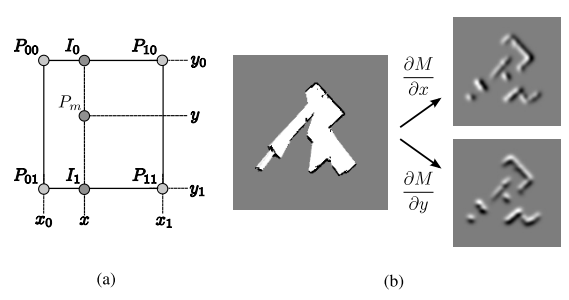
\includegraphics[width=0.7\linewidth]{figs/hectorSLAM_filtering}
%----------------------------------------------------	
	\caption[Hector SLAM aspects of filtering]{The figure illustrates aspects of filtering used to obtain sub-grid cell accuracy. (a) Bi-linear filtering of the occupancy grid map. Point $P_m$ is the point whose value shall be interpolated. (b) Occupancy grid map and spatial derivatives. Taken from \cite{Kohlbrecher2011a}.}
%----------------------------------------------------	
	\label{fig:hectorslamfiltering}
%----------------------------------------------------	
\end{figure}
%....................................................

%

%Equations \ref{eq:gaussnewton} and \ref{eq:hessian} rely on the gradient of the map \(\nabla{M}(P_m)\), where \(P_m\) is some coordinate in the map. Figure \ref{fig:hectorslamfiltering}illustrates the gradient approximation by a bilinear filter of the four closest coordinates(\(P_{00},P_{01}, P_{10},P_{11} \)) representing the midpoints of the surrounding map cells of \(P_m\). The gradient of the map can be approximated as
%\begin{equation}
%\frac{\delta{M}}{\delta{x}}(P_m) \approx (y-y_0)[M(P_{11} - M(P_{01}]+(y_1-y)[M(P_{10}) -M(P_{00})]
%\end{equation},

%\begin{equation}
%\frac{\delta{M}}{\delta{y}}(P_m) \approx (x-x_0)[M(P_{11} - M(P_{10}]+(x_1-x)[M(P_{01}) -M(P_{00}]
%\end{equation},

%where \(x, y \) are coordinates in the map of integer values \(P\). Another assumption is that %\(x_1 - x_0 = y_1 - y_0 = 1\) in the map coordinates.

%....................................................
\begin{figure}[H]
%----------------------------------------------------
	\centering
	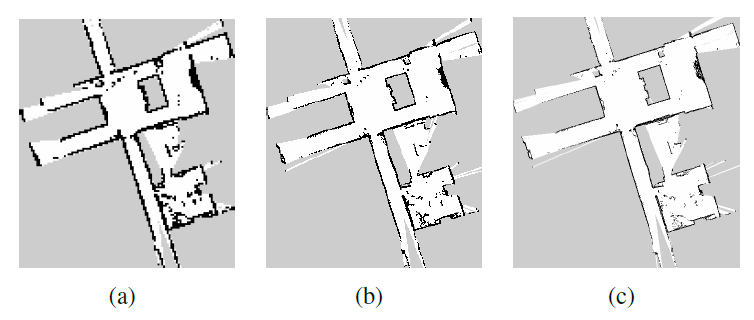
\includegraphics[width=0.7\linewidth]{figs/hectorSLAM_multiresolution}
%----------------------------------------------------	
	\caption[Hector SLAM multi-resolution representation]{Multi-resolution representation of the occupancy grid map: (a): 20 cm occupancy grid cell length (b) 10 cm occupancy grid cell length (c) 5 cm occupancy grid cell length. Where grey cells are unknown, black are occupied cells and white are unoccupied cells.Taken from \cite{Kohlbrecher2011a}.}
	\label{fig:hectorslammultiresolution}
%----------------------------------------------------	
\end{figure}
%....................................................

The scan matching is further optimised to reduce the effect of getting stuck in local minima as the procedure is based on gradient ascent. The optimisation is achieved by using \textit{image pyramids}, where the map is stored at different resolutions. Scan matching is then done at all levels of the image pyramid starting from the coarsest to finest representation. Instead of implementing a computationally costly method such as Gaussian filtering or down-sampling, at the different layers LIDAR scans are written at the scale of each map. The method of writing LIDAR scans to maps, ensuring computational effectiveness and consistency, see Figure \ref{fig:hectorslammultiresolution} \cite{Habbecke2006IterativeM}.

To help the scan matching algorithm, odometry and other position data sources can estimate the scan match. This initial estimation can be done with a Kalman filter or other methods of sensor fusion.

Hector SLAM discussed in this section solves the SLAM problem sufficiently accurately for both ground and water robots \cite{Kohlbrecher2011a}. Hector SLAM has proven to require half the computation time as FastSLAM requires \cite{Eliwa2017}. Furthermore, the approach does not require any explicit loop closing in the considered scenarios, due to  \cite{Kohlbrecher2011a}.  

%----------------------------------------------------
\subsection{Summary}

Even though all four paradigms discussed in previous sections perform in some instances, they have limitations associated with them, influencing the navigation block's performance, shown in Figure \ref{fig:autoover}. The fundamental needed for navigation in robots is an algorithm that covers high-level specifications of humans' tasks into low-level descriptions of how to move. For example, imagine being giving two computer-aided-design(CAD) models: a house and a piano. An algorithm is then expected to move the piano from one room to another without colliding with any obstacles. This problem is referred to as the \textit{Piano Mover's Problem} and defines the classic navigation problem \cite{lavalle_2006}.

Navigation's main objective is to move an object through the environment without collisions; the object and environment's current state needs to be accurately represented. Since the SLAM algorithm feeds the robot's current position and a local map to the navigation block, as shown in Table \ref{table:SLAM}. The quality of these need to be considered when selecting a SLAM algorithm. 

Shown in Table \ref{table:SLAM} are the limitations of the SLAM paradigms discussed in the previous sections. With a focus on data association, computational complexity and the ability to perform SLAM online. Hector-SLAM is selected in this work due to its robustness to loop closure, ability to perform SLAM online, and lack of dependency on odometry data, which is usually less accurate than modern LIDAR scanners. Furthermore, works done by \cite{Eliwa2017} shows that Hector-SLAM has higher accuracy than FastSLAM, even though its computation time is twice fast as FastSLAM. The representation of local maps passed to the navigation block will be discussed in the next section.

%....................................................
\begin{table}[H]
%----------------------------------------------------
\centering
\caption[SLAM method comparison]{A comparison of the reviewed SLAM methods, highlighting their advantages and disadvantages with regards to loop closure events, computational complexity, online capabilities and map size handling.}
    \begin{tabular}{p{6.5em}p{5.5cm} p{5.5cm}} 
%----------------------------------------------------
\toprule[1.5pt] 
%----------------------------------------------------
\multicolumn{1}{l}{\textbf{Method}}     & \multicolumn{1}{c}{\textbf{Advantages}}  & \multicolumn{1}{c}{\textbf{Disadvantages}} \\ 
%----------------------------------------------------
\midrule[0.5pt]
%----------------------------------------------------
  {\em EKF-SLAM }      & 
%....................................................    
        \begin{compactitem}{\small
%----------------------------------------------------    
        \item Works well with unique observations.
        \item Can perform SLAM online.}
%----------------------------------------------------        
    \end{compactitem}   & 
%....................................................   
    \begin{compactitem}{\small
%----------------------------------------------------    
        \item Computational complexity of $\mathcal{O}(M^2)$, where $M$ is the map size. This complexity makes EKF computationally expensive as the map grows to update the covariance matrix as the map grows.
        \item Susceptible to data association errors due to uni-modal pose representation. Hence, loop closure is more frequent.}
%----------------------------------------------------        
    \end{compactitem}\\
%....................................................
%----------------------------------------------------
\hline
%----------------------------------------------------
   {\em  FastSLAM  }     &
%....................................................    
    \begin{compactitem}{\small
%----------------------------------------------------    
        \item Overcomes the loop closure problem, with multi-modal data association.
        \item Copes well with nonlinear and non-Gaussian systems.
        \item Can perform SLAM online.}
%----------------------------------------------------        
    \end{compactitem}   &
%....................................................    
    \begin{compactitem}{\small
%----------------------------------------------------    
        \item Suffers from particle deprivation. Which limits long-term exploration.
        \item Becomes computationally expensive as the map size $M$ grows and the number of particles $Q$ increases, giving a computational complexity of $\mathcal{O}(Q \log M)$.}
%--------Q-, which -------------------------------------------        
    \end{compactitem}\\ 
%----------------------------------------------------
\hline
%----------------------------------------------------
   {\em GraphSLAM   }   & 
%....................................................    
    \begin{compactitem}{\small
%----------------------------------------------------    
        \item Ideal for building large-scale maps.
        \item Overcomes the loop closure problem.}
%----------------------------------------------------        
    \end{compactitem}   & 
%....................................................   
    \begin{compactitem}{\small
%----------------------------------------------------    
        \item Computationally expensive if not optimised. 
        \item Can not perform SLAM online effectively.}
%----------------------------------------------------        
    \end{compactitem}\\ 
%----------------------------------------------------
\hline
%----------------------------------------------------
  {\em   Hector SLAM }    &
%....................................................    
    \begin{compactitem}{\small
%----------------------------------------------------    
        \item Does not require loop closure.
        \item Hector SLAM depends on modern LIDAR scanners rather than odometry data which is less accurate. 
        \item Can perform SLAM online.
        \item Hector SLAM is two times fast computationally compared to FastSLAM \cite{Eliwa2017}.}
%----------------------------------------------------         
    \end{compactitem}   &
%....................................................    
    \begin{compactitem}{\small
%----------------------------------------------------     
       \item Initial guess of the pose may take longer to converge if odometry data are not used to initialise the scan matcher algorithm.} 
%----------------------------------------------------        
    \end{compactitem}\\
%....................................................
\bottomrule[1.5pt] 
%----------------------------------------------------
\end{tabular}
%----------------------------------------------------
\label{table:SLAM}
%----------------------------------------------------
\end{table}
%....................................................

%====================================================
\section{Map representation}
%----------------------------------------------------
The SLAM block discussed in the previous section produces both a local map and current robot pose in the map. The representation of the map depends on how the map is going to be used. For example, in the \textit{Piano Mover's Problem} discussed in the previous section, a piano requires moving from room to room. In this case, our assumptions will be a three-dimensional environment with room labels. In other examples, robots may need all objects in the environment labelled. Therefore, an effective map representation is required to match the scenario. In the case of this thesis, the map representation needs to be compatible with merging maps generated from multiple robots to form a global map of the environment. 

There are various types of map representations, varying from geometrical to logical maps which have been developed to date; the following factors characterise the complexity of mapping problem \cite{Thrun2006}:

%....................................................
\begin{itemize}
%----------------------------------------------------
    \item \textbf{Size}: If the environment size is larger than the relative perceptual range of the robot, mapping becomes more difficult. This makes it more challenging to compute the full posteriors over maps.
%----------------------------------------------------
    \item \textbf{Noise perception and actuation}: Noise on the sensors and actuators of the robot decreases the accuracy, as the errors accumulate.
%----------------------------------------------------
    \item \textbf{Perceptual ambiguity}: If different locations look-alike more frequently, it is more difficult to establish a correspondence between the locations at different time points.
%----------------------------------------------------
    \item \textbf{Loop Closure}: With odometry error, it is easier to correct if the robot travels up and down a corridor. The difficulty comes when a robot re-enters a location from a different path. This same problem was a point of discussion in the previous sections.	
%----------------------------------------------------
\end{itemize}
%....................................................

%----------------------------------------------------
\subsection{Occupancy grid maps}
%----------------------------------------------------
Occupancy grid maps were first introduced in the 1980s and are one of the most common map representations \cite{Siciliano2008b}. In the approach is represented by discrete cells. Where the posterior probability is calculated to determine if a cell is occupied or not, in the case of range sensors, cells will be empty if rays are unobstructed and rays that have an endpoint will be observed as occupied. Occupancy grid maps also account for unknown space, where the area of the map has not been explored as yet. Figure \ref{fig:exampleofoccupancygrid} is an example of an occupancy grid map created using a laser range finder. Black represents occupied cells, white represents empty cells, and grey represents unexplored territory.

%....................................................
\begin{figure}[H]
%----------------------------------------------------
	\centering
	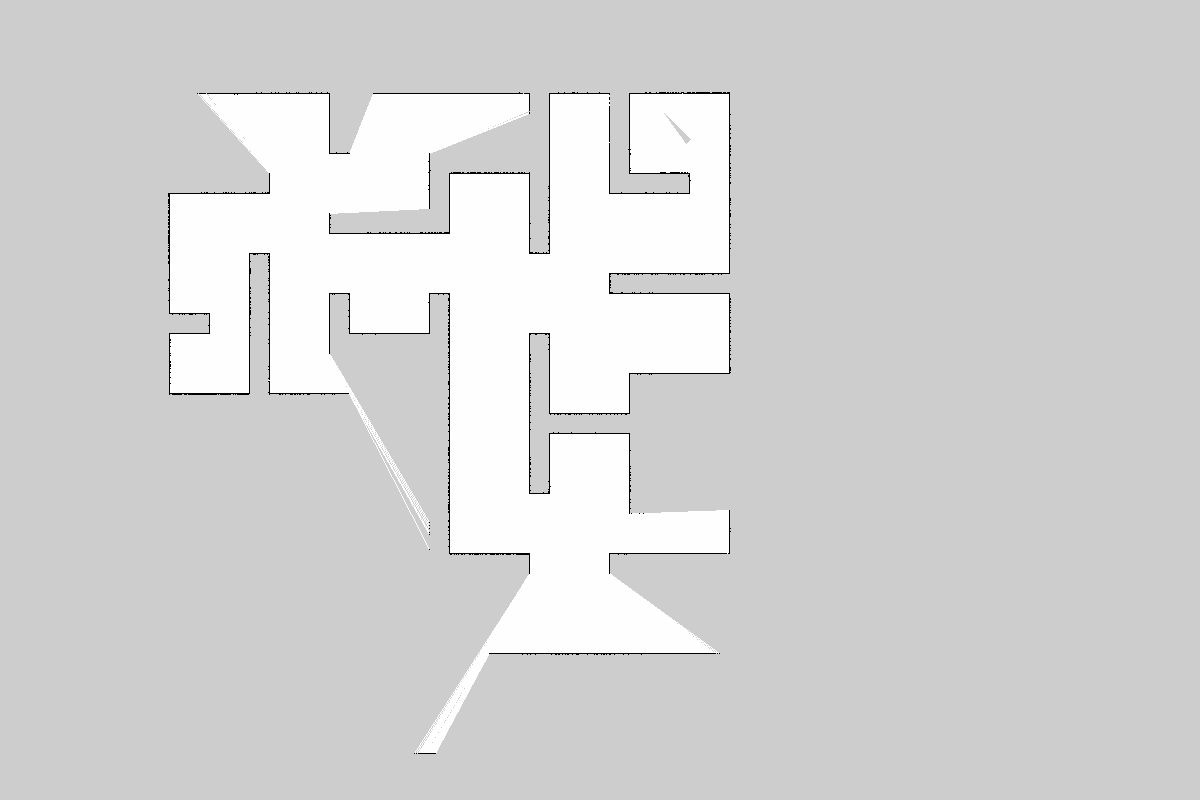
\includegraphics[width=0.7\linewidth]{figs/example_of_occupancy_grid}
%----------------------------------------------------	
	\caption[An example of an occupancy grid map]{An example of an occupancy grid map, which was produced in simulation using Gazebo and ROS (explanation of how the data were acquired is explained in further chapters). Black represents occupied cells, white represents empty cells, and grey represents unexplored territory.}
	\label{fig:exampleofoccupancygrid}
%----------------------------------------------------	
\end{figure}
%....................................................

During an exploration, new sensor observations are used to update the grid cells according to the \textit{Binary Bayes Filter}. The belief of a particular cell \(\mathbf{m}_i\) is given by:

\begin{equation}
%----------------------------------------------------
    bel_{k}(\mathbf{m}_i) = P(\mathbf{m}_i|\mathbf{z}_{1:k},\mathbf{x}_{1:k}),
%----------------------------------------------------
\end{equation}

where ,$\mathbf{m}$, represents the entire map, $\mathbf{m}_i$, is an individual cell in the map, $\mathbf{z}_{1:k}$, is a set of measurements and $\mathbf{x}_{1:k}$ is the pose of the robot at time ,$k$. Therefore the belief for the entire map ,$\mathbf{m}$, is given by:
%....................................................
\begin{equation}
%----------------------------------------------------
    bel_{k}(\mathbf{m}) = \prod_{i}P(\mathbf{m}_i|\mathbf{z}_{1:k},\mathbf{x}_{1:k}).
%----------------------------------------------------    
\end{equation}
%....................................................
A common approach is to represent the belief using \textit{log-odds} \cite{Thrun2001b}:
%....................................................
\begin{equation}
l_{k,i} = \log \frac{P(\mathbf{m}_i|\mathbf{z}_{1:k},\mathbf{x}_{1:k})}{1-P(\mathbf{m}_i|\mathbf{z}_{1:k},\mathbf{x}_{1:k})},
\end{equation}
%....................................................
the \textit{log-odds} representation is used to avoid numerical instabilities for probabilities near zero or one. The probabilities can be recovered using:
%....................................................
\begin{equation}
%----------------------------------------------------
P(\mathbf{m}_i|\mathbf{z}_{1:k},\mathbf{x}_{1:k}) = 1 - \frac{1}{1 + \exp {l_{k,i}}}.
%----------------------------------------------------
\end{equation} 
%....................................................
Finally combining the \textit{log-odds} beliefs can be represented as:
%....................................................
\begin{equation}
%----------------------------------------------------
    l(\mathbf{m}_i|\mathbf{z}_{1:k},\mathbf{x}_{1:k}) = l(\mathbf{m}_i|\mathbf{z}_{1:k-1},\mathbf{x}_{1:k-1}) + l(\mathbf{m}_i|\mathbf{z}_{k},\mathbf{x}_{k}). 
%----------------------------------------------------
\end{equation}
%....................................................

The advantage of these types of maps is that they can handle the dynamic environment, do not rely on predefined features, offer constant-time access to grid cells, and represent unobserved areas \cite{Siciliano2008b, Saeedi}. However, when dealing with dynamic environments, the drawback is that unlearning that a cell is free requires as much observation as the robot received to declare the area occupied \cite{Siciliano2008b}.

These maps also have disadvantages which mainly pertain to high memory requirements (when working in higher dimensions). Therefore, even though 3D maps (called voxels) can be represented using this representation, the implementation will have high memory costs\cite{Saeedi}.

%----------------------------------------------------
\subsection{Feature (as known as landmark) maps}
%----------------------------------------------------
When environments have distinguishable features such as a pillar or tree, for example, landmark-based map representations are typically used. Signatures of the features are usually used to occupy the position of the feature. This representation is more efficient of localisation as the landmark features are initially defined, but feature extraction (data association) is the drawback to this implementation\cite{Siciliano2008b}.
%----------------------------------------------------
\subsection{Topological Maps}
%----------------------------------------------------
Topographical representation was firstly presented in work done by \cite{Kuipers1991} and is one of the more popular mapping techniques. This technique represents the environment in a graph-like structure, focusing on the geometric structure of the environment. In topological mapping, unique, distinguishable places are defined as nodes, and the connections between the nodes are edges where the robot can travel \cite{Siciliano2008b}. 

Topological maps can also be derived from metric maps such as occupancy grids. An example of a Voronoi graph topological map presented in \cite{2005i} produced a topological map from an occupancy grid map. A metric-free topological maps approach is introduced in \cite{Derenick2013}, enabling minimalistic robot localisation.

Note that topological maps are well suited for high-level planning but need intensive map processing, and they are limited in way-point following \cite{Saeedi}.

%----------------------------------------------------
\subsection{Summary}
%----------------------------------------------------
In selecting the appropriate representation for this work, the representations need to be favourable for both map merging and navigation (see Table \ref{table:maprep} for characteristics of the different approaches). Thus, occupancy grid map representation has been selected for their flexibility when representing the environment, and do not require as much computational ability as Feature and Topological maps \cite{Thrun2006}. In the case of map merging, they allow for image registration, and optimisation based approaches \cite{Saeedi}. Occupancy grid maps can also be abstracted to topological maps for navigation \cite{Saeedi}.
%....................................................
\begin{table}[H]
%----------------------------------------------------

\centering
\caption{Map representation characteristics}
\label{table:maprep}
%----------------------------------------------------
\footnotesize
\begin{tabular}{p{4.5em} p{5.5cm} p{4cm} p{4cm}} 
%----------------------------------------------------
\toprule[1.5pt] 
%----------------------------------------------------
\multicolumn{1}{l}{\textbf{Type of Map}} & 
\multicolumn{1}{c}{\textbf{Characteristics}} &
\multicolumn{1}{c}{\textbf{Pros}} &
\multicolumn{1}{c}{\textbf{Cons}}  \\ 
%----------------------------------------------------
\midrule[0.5pt]
%------{\em Occupancy Grid Maps}---------------------	
		{\em Occupancy Grid Maps} &
%....................................................   
		The map is defined as a grid, where each cell is either occupied, free or unknown. &
		
%.................................................... 	
        It is easy to build, probabilistic, suitable for 2D maps, easy to maintain, and suited for low-level planning. & Expensive on fine resolutions and 3D representations, exponential cost of memory with growing size. \\
%....................................................
%----------------------------------------------------
\hline
%----------------------------------------------------
		{\em Feature Maps} & 
%....................................................		
		Maps are represented by landmarks such as trees and shapes. & 
%....................................................
		Very useful for localisation. & Requires computationally expensive data association.\\
%....................................................
%----------------------------------------------------
\hline
%----------------------------------------------------
		{\em Topological Maps} & 
%....................................................
		Abstract spacial information is used to represent the maps. & 
%....................................................
		It is suited for high-level planning. & Is limited to way-point.\\
%....................................................
\bottomrule[1.5pt] 
%----------------------------------------------------		
	\end{tabular}
%----------------------------------------------------	
\end{table}
%....................................................

%====================================================
\section{SLAM extended to Multiple Robots}
\label{sec:SLAMMR}
%----------------------------------------------------
This section will briefly describe multiple-robot systems and multiple-robot SLAM. Generally, multiple robot SLAM algorithms are built on top of single robot SLAM systems; therefore, methods and map representation are based on the approaches mentioned previously. Jung suggests that the following advantages drive research in the field of multiple-robot SLAM \cite{Jung2000}:
%....................................................
\begin{itemize}
%----------------------------------------------------
\item \textbf{Space and time distribution} - Multiple robots can be in many places while performing different tasks simultaneously. This allows robots to, for example, explore a vast area in a shorter period.
%----------------------------------------------------
\item \textbf{Simpler is better} - In the multiple agent case, each robot can be more straightforward rather than have a single agent that is complex. This simplicity not only decreases the cost of each agent but increases reliability and robustness (see Figure \ref{fig:relvscomp}).
%----------------------------------------------------
\item \textbf{Divide and conquer} - Certain problems are best solved when divided into smaller problems and distributed among the robots.
%----------------------------------------------------
\end{itemize}
%....................................................

%....................................................
\begin{figure}[H]
%----------------------------------------------------
    \centering
    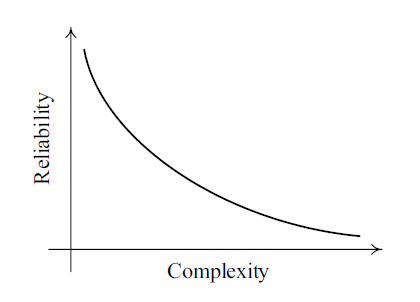
\includegraphics{figs/relability_vs_complexity.png}
 %----------------------------------------------------   
    \caption[Relationship between reliability and complexity]{Relationship between reliability and complexity. The figure suggests that the simpler the system, the more reliable it is. Taken from \cite{Jung2000}.}
    \label{fig:relvscomp}
%----------------------------------------------------    
\end{figure}
%....................................................

However, having a multiple robots system has its associated problems. According to \cite{Saeedi}, these are the potential problems:
%....................................................
\begin{itemize}
%----------------------------------------------------
    \item \textbf{Relative poses} - Maps produced by individual autonomous robots are referred to as local maps, which are produced in the robot's frame of reference. To produce a global map, each robot needs to incorporate maps from all the robots. This can be difficult as it requires transformation matrices to relate the maps to each other. The relative pose also has its associated uncertainty which can be represented as a covariance matrix. This uncertainty can be caused by modelling, sensor noise, and linearisation effects \cite{Thrun2006}. 
%----------------------------------------------------    
    \item \textbf{Updating maps and poses} - After the relative transformation matrix has been found, the local maps need to be fused; thus, the poses also need to be updated. The process needs to consider the robot trajectory and new information added to the local maps. The processes also need to consider the type of map; for example, in feature-based maps, duplicate landmarks may need to be removed \cite{Siegwart2004}.
 %----------------------------------------------------   
    \item \textbf{Line-of-sight observations} - Line-of-sight observation is when robots can see or detect each other. Even though robots might already possess the other robots' pose estimation, line-of-sight can improve the estimates.  In some cases, this can be more reliable than the indirect approaches, but in some cases, robots might not have a sight of each other, especially during a mission such as search and rescue \cite{DeHoog2009}. Furthermore, line-of-sight has been used in loop closure scenarios \cite{Matari2004}.
%----------------------------------------------------    
    \item \textbf{Loop closure} - This happens when a robot revisits a previously visited location but not very recently. As the issue is already complicated enough for single robot missions \cite{Balcilar2016}, extending this to multiple robots, the issue requires information from the robots in the system to be solved \cite{Howard2006a}.
 %----------------------------------------------------   
    \item \textbf{Complexity} - Especially when considering that usually robotic applications are real-time, space and time advantages mentioned above are essential to solving the multi-robot SLAM problem with minimum time and memory requirements. This complexity directly affects the scalability of the multi-robot SLAM operation.
%----------------------------------------------------    
    \item \textbf{Information sharing} - The quality of the information sharing among the robots mainly depends on the medium and environment which they are communicating \cite{Carlone2010a}. For example, underwater robots face different issues to that of aerial robots. Different environments introduce different limitations to bandwidth, data rate and throughput.
%----------------------------------------------------    
    \item \textbf{Homogeneous vs. heterogeneous} - Having a diverse robot team can be a considerable advantage, especially in different terrain environments, this allows for a wholesome model of the environment. For example,  a team may have robots on the ground, in the air and underwater \cite{Siciliano2008b}. The synchronisation between the different robots and sensors, is an essential part of multiple robot systems, firstly on each robot and all the robots. However, this advantage requires processing and integrating different types of robots \cite{Wurm2012}, such as integrating different map representations.
 %----------------------------------------------------   
    \item \textbf{Performance measure} - Measuring the accuracy of multiple robot systems, can be challenging considering the issues mentioned above and the lack of a model of the environment. This process is essential, primarily if the robot relies on SLAM to coordinate and perform tasks. Performance measures can be used to ensure the reliability of multiple-robot SLAM systems.
%----------------------------------------------------    
\end{itemize}
%....................................................

Furthermore, in Multiple Robot SLAM can either be centralised or decentralised \cite{Leung2010}. In a \textbf{centralised system}, there is a predetermined robot in the team or an external agent which handles the computation of tasks. The assumption is that the central agent has a global map of the ``World'', which theoretically means that the central agent can optimally allocate tasks to the robot team. The robots would need to send partial maps continuously to the central agent, and the central agent will be responsible for aligning and merging the maps then the maps would be sent back to the robot team to produce the global map. This requires constant communication between the robot's in the team and the central agent. The central approach can either be implemented wholly (apart from the central agent other, agents have no control or autonomy) or partially (there is still a central agent, but other agents can also take some autonomous local decisions). 

In a \textbf{decentralised system}, more than one robot is tasked with performing computations for tasks. However, it requires each robot to have adequate computational ability to act independently. In the map merging case, the robots may exchange maps with each other then align and merge them internally. The global map built by each robot may vary depending on which robots they have exchanged information.

Centralised systems allow for coherent and comprehensive solutions. However, depending on the size of the team in a centralised system it may become difficult or impractical to store all the information of the environment on one agent \cite{Leung2010}, a communication bottleneck may arise due to the massive communication between the central agent and other agents, high complexity leads to low reliability as per the following Figure \ref{fig:relvscomp}. On the other hand, a decentralised system is tolerant to failure, reliable and robust, scalable, and tasks can be decomposed and run in parallel compared to the centralised approach \cite{Leung2010}.

In this section, the advantages and disadvantages of Multiple Robot SLAM are discussed. In the next section, related work on Multiple Robot SLAM is discussed concerning these advantages and disadvantages.

%====================================================
\section{Related work on Multiple Robot SLAM}
%----------------------------------------------------
In the previous section, three key advantages (space and time distribution; simplicity; and divide and conquer) and eight fundamental problems (relative poses of robots; uncertainty of the relative poses; updating maps and poses; line-of-sight observations; closing loops, complexity communications; team diversity; synchronisation and performance measures) of multiple-robot SLAM were discussed, which are adapted from \cite{Saeedi}. Furthermore, the centralised vs. decentralised multiple-robot SLAM systems are discussed. The following section will explore multiple-robot SLAM solutions.

Several researchers proposed the Multi-Robot SLAM problem, with work dating back to the early 2000s such as \cite{Nettleton2000}. \cite{Nettleton2000} applied the information formulation to the multiple-robot SLAM problem; the work shows that the Extended Information Filter (EIF) is more suitable than EKF multiple-robot SLAM since the information has the additivity attribute. However, the authors noted that data association and communication between robots would need to be further researched.  

Later \cite{Thrun2005} improved on the work done by \cite{Nettleton2000}, by proposing a multiple-robot SLAM with Sparse Extended Information Filers (SEIF). An algorithm that enables robot teams to build joint maps where the relative starting position is unknown and landmarks are ambiguous. The alignment of local maps to generate a global map is achieved by a tree-based algorithm which searches for local landmarks arrangements combined with a hill-climbing method to maximise the overall likelihood. 

Fenwick et al. propose an EKF based multiple-robot SLAM approaches and explore merging sensor and navigation information from multiple robots \cite{Fenwick2003}. The method is based on stochastic estimation and uses a feature-based map representation, where a theoretical convergence theorem is proved for the first time. This approach quantifies gains of using a team of robots, therefore determining the number of robots required in a team to perform tasks.

Another EKF based multiple-robot SLAM technique is proposed by \cite{Rekleitis2001}, where a team of robots (both stationary and dynamic) directly observe each other to reduce the dead reckoning errors. Furthermore, the algorithm is designed to cope with hard-to-sense reflectance properties. 

Later, \cite{4058636} proposed an EKF based multiple-robot SLAM technique, which aimed to solve the with the aid of robots rendezvousing to consolidate the relative position. In the method, robots do not require knowledge of their initial relative poses to merge maps to form a joint map. Furthermore, the method optimises the map merging and not the map overlap. 

In \cite{Andersson2008}, a multiple-robot SLAM method using Square Root Information Smoothing is presented. This method allows a team of robots to built a global without initial information of the robots relative poses, during a line-of-sight observation. In contrast to EKF approaches, the smoothing is better equipped to deal with the nonlinear process and measurement models. The method joins the maps from different robots and recovers each robot's complete trajectory in the map merging process.

In 2001 Thrun \cite{thrun2001a} proposed a multiple-robot SLAM solution based on a particle filter, where the fast maximum likelihood map grows with a Monte Carlo localiser that uses a particle representation. This yields an online algorithm that can cope with significant odometric errors, typically found when dealing with loop closures. However, the method has the following limitations: firstly, it cannot handle nested cycles in the map, secondly does not deal well with lower quality range sensors such as sonar sensors, and thirdly robots need to know their initial relative poses to each other.  

Later in 2006, the work was extended by \cite{Howard2006a}, where a multiple-robot SLAM using Rao–Blackwellised particle filter was proposed. The robots use line-of-sight to estimate relative position, using cameras and unique markers mounted on them. At the first meeting point, a Rao–Blackwellised particle filter (RBPF) is applied to the data in reverse time sequence to fuse all the data from the starting point, to determine relative position. Furthermore, the maps and poses are updated in real-time, and the decentralised nature of the system increases reliability, robustness and the scalability of the approach. However, it cannot be applied if the robots cannot see each other, and are unable to determine their relative positions. 

Carlone \cite{Carlone2010a} similarly explores multiple-robot SLAM using the RBPF extending on \cite{Howard2006a}'s work relative initial position of the robots are unknown. In this work, the main focus is information sharing among the robots, with limited communication between them. The information shared when the robots are in-range includes all the odometry and corresponding laser range-finder data. Line-of-sight observation is used then to compute the relative pose with an incorporated uncertainty. 

In \cite{VidalCalleja2011}, a heterogeneous multiple-robot SLAM algorithm using sub-map matching is developed on a team of robots comprised of one ground robot and a helicopter. A global graph maintains the relative relationships between the local sub-maps. Monocular cameras are used as the primary exteroceptive sensors in this work. 3D points are estimated using an inverse-depth parametrisation, 3D line segments are estimated by adding endpoints to extend anchored Pl\"ucker coordinates (a coordinate system that assigns six homogeneous coordinates to each line in projective 3D-space\cite{ZHAO2014113}).

In \cite{Quraishi2016}, robustness to connectivity loss for multiple-robot SLAM method is proposed. In the framework, no central authority is required while the robot team contributes to the global map. However, this method requires systematic coordination among the robots in order to add to the global map. Hence, if a robot leaves the system unannounced, it can potentially make the map inconsistent.

Work done by \cite{Balcilar2016} proposes a Hector mapping architecture for multi-robot. In their work (which they implemented in ROS), each robot shares its observations and poses a central note. The central node computes the global map, using the poses (including the initial poses) and observations from the robot team. Furthermore, parallelising optimisation steps and sequentially registering laser scans to the jointly built map are implemented to enable real-time running. Table \ref{table:multisolution} states the algorithms' main features in this section.
%....................................................
\begin{table}[H]
%----------------------------------------------------
    \centering
    \caption{Solutions to Multiple Robot SLAM problems }
%----------------------------------------------------
\begin{tabular}{p{5cm}p{5.5cm}} 
%----------------------------------------------------
    \toprule[1.5pt]
%----------------------------------------------------   
\multicolumn{1}{l}\textbf{Problem} & 
\multicolumn{1}{c}\textbf{Solutions}\\ 
%----------------------------------------------------    
    \midrule[0.5pt]
 %----------------------------------------------------   
    {\em Relative poses}        & 
    \cite{Thrun2005}, \cite{4058636}, \cite{Rekleitis2001}, \cite{Carlone2010a}, \cite{VidalCalleja2011}, \cite{Quraishi2016}\\ 
%----------------------------------------------------     
   % \hline 
   & \\  
%----------------------------------------------------   
   {\em Updating maps and poses}      & 
   \cite{Thrun2005},\cite{Fenwick2003},\cite{Howard2006a}, \cite{VidalCalleja2011}, \cite{Andersson2008}, \cite{Quraishi2016}\\
 %---------------------------------------------------- 
    %\hline
     & \\  
 %----------------------------------------------------   
    {\em Line-of-Sight observations}  & 
    \cite{Rekleitis2001},\cite{4058636},\cite{Howard2006a}, \cite{Andersson2008}\\
 %----------------------------------------------------   
    %\hline
     & \\  
 %----------------------------------------------------   
     {\em Loop closure}               & 
    \cite{Rekleitis2001}, \cite{thrun2001a}\\ 
 %----------------------------------------------------   
  %  \hline
   & \\  
 %----------------------------------------------------   
     {\em Complexity}               & 
    \cite{Howard2006a}, \cite{Balcilar2016}, \cite{Andersson2008}\\
 %----------------------------------------------------
   %  \hline
    & \\  
%----------------------------------------------------     
     {\em Information sharing}         & 
    \cite{Carlone2010a}, \cite{Quraishi2016}\\
 %----------------------------------------------------
   % \hline
    & \\  
%----------------------------------------------------   
    {\em Homogeneous vs. Heterogeneous} & 
    \cite{VidalCalleja2011} \\
 %----------------------------------------------------   
   % \hline
    & \\  
 %----------------------------------------------------   
    {\em Performance measures}         & 
   \cite{Fenwick2003}\\
%----------------------------------------------------    
    \bottomrule[1.5pt]
%----------------------------------------------------   
\end{tabular}
%----------------------------------------------------
\label{table:multisolution}
%----------------------------------------------------
\end{table}
%....................................................

%====================================================
\section{Summary}
%----------------------------------------------------
In this chapter, an overview of SLAM is explored, including SLAM formulation, single robot SLAM solutions, map representation, and multiple-robot SLAM extension. The multiple-robot SLAM literature, problems such as relative poses, updating maps and pose and homogeneous vs. heterogeneous are discussed in Section\ref{sec:SLAMMR}, along with some solutions that tackle the problems. The work done in this chapter, also prompts the use of Hector SLAM as the SLAM algorithm each robot will be equipped; occupancy grid maps as the map representation; and a distributed architecture where robots communicate when they discover each other in the network. In the next chapter, merging maps from single independent robots are discussed, along with details on how maps are acquired, how robots share maps, and how they are aligned and merged.
%****************************************************
% END
%****************************************************
 % SLAM overview
% !TeX spellcheck = en_GB
%****************************************************
%	CHAPTER 3 - Map Merging
%****************************************************
\chapter{Map merging}
\label{sec:map-merging}
%----------------------------------------------------
This chapter discusses map merging for multiple robots; the discussion includes reviewing the literature and parameter tuning experiments. In multi-robot SLAM, two or more robots explore an environment independently and generate local partial maps. Merging of all the partial maps to form a global map, is functional to applications such as finding frontiers for all the robots in the environment \cite{Burgard2000}. Map merging can be simplified into two steps which involves finding alignments (such as rotation, resolution and translation) between maps, and then merging maps using information from the first step. The maps and other information about the robots are shared to find the alignment between the different maps in the steps mentioned. The focus, as mention in the previous chapter, is on merging 2D occupancy grid maps.

%====================================================
\section{Problem statement}
%----------------------------------------------------
Consider a large and complex environment, where a team of robots is tasked to maps different parts of an environment at different grid map resolutions. The resolution is defined by a metric $x$ per cell; in this work, we will be using meters/cell (m/cell), which is the size in meters of an individual grid map cell. The partially overlapping local grid maps generated from the task must be integrated into a global map that can be useful for robots to perform operations such as path planning and frontier finding.

\subsection{Definitions}

Definition 1: Let $\mathbf{m}$ be a map of $N$ by $M$, where $N$, $M$ are positive real numbers:

\begin{equation}
    \mathbf{m}: [0, N] \times [0, M] \rightarrow \mathbb{R}
\end{equation}

We can also denote a set of $N$ by $M$ maps as $\mathbf{I}_{N \times M}$


Definition 2:  According to \cite{Carpin2008b}, the goal of pairwise map merging is to find a relative transformation denoted by:

\begin{equation}
    \mathbf{T}_{t_x,t_y,\theta} = \begin{bmatrix}
            s\mathbf{R} & \mathbf{t}\\
            0 & 1
        \end{bmatrix}
        \label{eq:transformation}
\end{equation}

, where $s \in \mathbb{R}$ is the scale factor, $\mathbf{R} \in \mathbb{R}^{2\times2}$ represents a two-dimensional counterclockwise rotation matrix about origin point ($x,y$) of $\theta$ angle $\theta$ and $\mathbf{t} \in \mathbb{R}^2$ indicates a translation vector ($t_x, t_y$). More specifically, $\mathbf{R}$ and $\mathbf{t}$ can be denoted as follows:

\begin{equation}
    \mathbf{R} =  \begin{bmatrix}
        cos(\theta) & sin(\theta)\\
        -sin(\theta) & cos(\theta)
        \end{bmatrix},
    \mathbf{t} = \begin{bmatrix}
        t_x\\
        t_y
        \end{bmatrix}
\end{equation}

Definition 3:  
Let $\mathbf{m}_1, \mathbf{m}_2, \dots, \mathbf{m}_k$ be $k$ maps in $I_{N \times M}$
\begin{equation}
    \omega(\mathbf{m}_1, \mathbf{m}_2) = \sum_{i=0}^{N-1}\sum_{j=0}^{M-1} Eq(\mathbf{m}_1[i,j], \mathbf{m}_2[i,j]).
\end{equation}

Here $Eq(a,b)$ is one when a=b and zero otherwise, and $\omega$ is an overlapping function that measures how much the two maps agree. In an ideal world, robots would cover the same area, where there exists a transformation which yields $ \omega(\mathbf{m}_1, \mathbf{m}_2) = N \times M$. In the real world this is not the case, so the objective is to find the transformation which maximises overlap. Therefore, ${x, y, \theta}$-map transformation, $\mathbf{T}_{t_x,t_y,\theta}$ is determined by maximising $ \omega(\mathbf{m}_1, \mathbf{T}_{t_x,t_y,\theta}(m_2))$.

Suppose there are a couple of overlapping maps: the subject map $\mathbf{P}$ and the seed map $\mathbf{Q}$, which have different resolutions built by robots exploring two parts of the same environment. To merge the seed map $\mathbf{Q}$ into map $\mathbf{P}$, a transformation $\mathbf{T}_{t_x, t_y, \theta}(x, y)$ is applied to map $\mathbf{Q}$, to obtain new map $\mathbf{Q}^{'}$ indicated as $\mathbf{Q}^{'} = \mathbf{T}_{t_x, t_y, \theta}(x, y) \mathbf{Q}$. Once transformed map $\mathbf{P}$ and $\mathbf{Q}^{'}$ are then merged to form a global map. The following section explores solutions to solving the map merging problem defined in this section. 

\section{Related work}

Various solutions are presented in the literature for maps from a team of mobile robots. The following four cases, where most are discussed in \cite{Rone2013} are used to study map merging in this section:
 
\begin{enumerate}[a.]
	\item \textbf{Known initial configuration}: This case is the simplest as the initial pose of the robots is known, which simplifies the map alignment step. This assumption is a limited case as many times the initial poses are not known as described in \cite{Carlone2010a}. In the case of Figure \ref{fig:initial}, for the initial poses to be known, the relative pose would be described by the distance between $G_i$ and $G_j$.
	\item \textbf{Rendezvous}: This case is where two robots meet at a point such as in Figure \ref{fig:rendevous}, where the relative pose is calculated using methods such as line-of-sight measurement. The distance between the robots determines the accuracy at the meeting point and the method used to compute the relative distance. However, this adds a level of complexity to the system as either the robots need to coordinate a meeting point or use a method such as an image processing to recognise other robots \cite{4058636}.
	\item \textbf{Relative position estimation}: In this case, a robot localises other robots in its local map. The critical element to this case is that there is no need for the robots to rendezvous or have knowledge of initial relative positions \cite{1249654}.
	\item \textbf{Overlaps}: In this case, overlaps in the map are used to calculate the relative transformation between different maps such as in Figure \ref{fig:overlap}. The main challenge is finding the maps' overlaps using features such as doors, junctions or corners. The optimal algorithm is one that can identify both false and true matches, in the least amount of time with the highest accuracy \cite{Birk2006}.
\end{enumerate}

\begin{figure}[H]
    \centering
    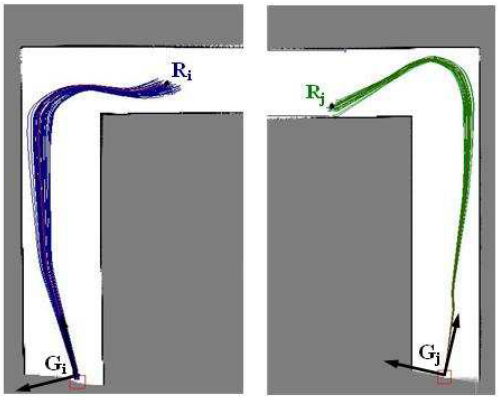
\includegraphics[width=0.5\textwidth]{figs/initial_configuration_example.png}
    \caption[Two relative robot maps]{This figure shows an example of two robots with unknown initial configurations. Each robot estimates both trajectory and map hypotheses in its own reference frame. In the case where initial configuration is known, the relative distance between $G_i$ and $G_j$ is known. Taken from \cite{Carlone2010a} }
    \label{fig:initial}
\end{figure}

\begin{figure}[H]
    \centering
    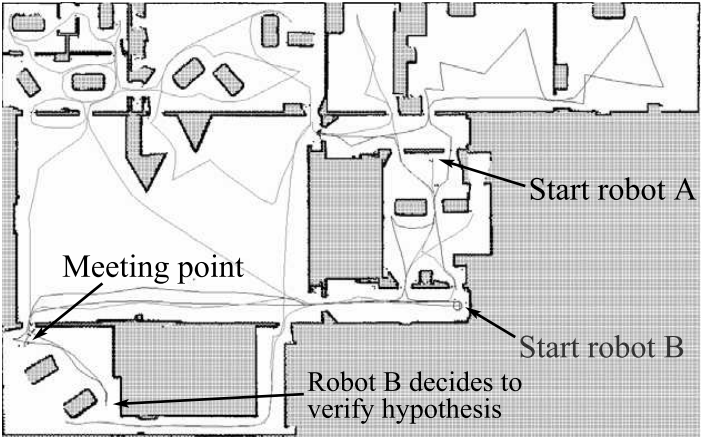
\includegraphics[width=0.5\textwidth]{figs/rendezvous_example.png}
    \caption[Example of coordinated exploration]{Example of a coordinated exploration of an unknown environment, from unknown locations. When then the robots meet at the meeting pint, they estimate and verify relative locations using a rendezvous approach. At the meeting point they share a map and their coordinate. Taken from \cite{Thrun2006}.}
    \label{fig:rendevous}
\end{figure}

\begin{figure}[H]
    \centering
    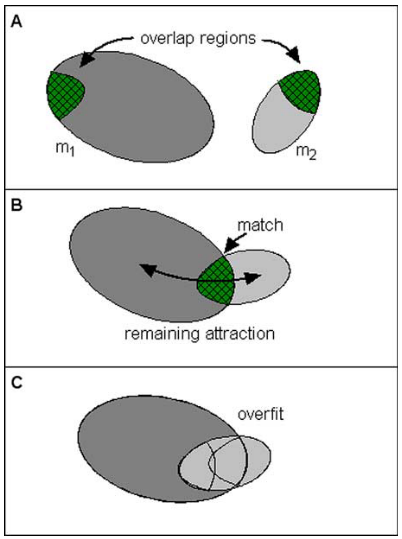
\includegraphics[width=0.5\textwidth]{UCT_MSc_Thesis/figs/overlap_example.png}
    \caption[Overlap matching example]{(A) describes the overlap region of the $m_1$ and $m_2$, where similarity is maximised. In (B) the identical regions are matched, where the unmatched regions remain unchanged. (C) is an example of over-fitting, where an area without a match is merged into another map. Taken from \cite{Birk2006}.}
    \label{fig:overlap}
\end{figure}


Early strategies of solving map merging with multiple robots such as \cite{Burgard2000} assume a known initial position of the robots. Although this method required minimal computational power, the method will fail if robots are unaware of each other's initial position. The more flexible approaches started presenting themselves in \cite{Carpin2005}, where map merging was solved as an optimisation problem. The authors in \cite{Carpin2005}, proposed a stochastic search approach to solve the problem. This method is an exhaustive approach based on adaptive random walks aiming to find suitable transformation to overlap the maps. Work was further done by \cite{Birk2006a} to improve the algorithm, and the improvement attempts to detect failures and guide the search to find the optimal solution. However, the exhaustive nature of the algorithm makes it computationally expensive to implement.

Xin Ma et al. later proposed a generic adaptive algorithm implemented without standard reference frames and relative pose information of robots \cite{XinMa2008}. The authors claim that their algorithm outperforms one presented by \cite{Carpin2005} because the generic adaptive algorithm can search the optimal match overlapping area more effectively. Avoiding premature convergence, low convergence speed and low stability. However, they did not present a merging of complex real-world maps, and the experimental results are of simple simulation maps. 

Saeedi et al. propose an artificial intelligence-based approach to map merging  \cite{Saeedi2011a}. The algorithm clusters the maps using neural-networks based on self-organised map (SOM); the cluster norms are used to find the relative transformation between the maps. Although this reduces dimensionality and improves processing time, the downfall is that some information is lost in the process. Dinnissen et al. proposed another artificial intelligence-based novel approach using reinforcement learning; the model is trained to determine a policy capable of deciding the best merge \cite{Dinnissen2012}. This approach allows the robot to incur less error during merging compared to simply merging after alignment. However, the model is validated using a simulated dataset instead of a real-world dataset.
 
Blanco et al. proposed a novel map-matching algorithm from image registration \cite{Blanco2013}. In this method, the maps are represented both as points and occupancy grid maps. The grid maps are firstly matched then the corresponding point maps are matched to help remove false matches. The transformation is determined by removing high-frequency noise and using feature detectors such as Harris or Kanade Lucas Tomasi (KLT). Matches are then filtered using a customised RANSAC algorithm based on the sum of Gaussian distributions. Based on the experimental results, this method deals adequately with uncertainty and ambiguity when matching maps.

Alternatively, Hough transforms are a way of representing geometrical data within maps. \cite{Carpin2008} proposes a Hough spectrum-based approach which was first introduced by \cite{1570528}. The maps are transformed into the Hough space, and the resulting Hough images are then correlated to find the potential transformations (rotation/translation). The authors introduce an acceptance index which tells how well-aligned maps are for each transformation. This index has values between 0 and 1, where 1 is a correct transformation, and 0 is an incorrect transformation. However, this solution fails when there is not enough overlap between maps. \cite{Saeedi2014c} further improved the approach by adapting the new cross-correlation operator allowing the algorithm to deal with less overlap in the maps.

Topology is a field of mathematics that studies the properties preserved through stretching, deforming, and twisting of an object \cite{Kuipers1991}. Topologies can be used in mapping to abstract objects while ignoring details. Topological maps can use a graph to represent navigation possibilities through an environment, where vertices are ``places'' and edges represent paths between the``places''. Even though maps can lose information from this abstraction, it can improve communication and mutual perception. Topological approaches have applications in map merging such as \cite{Huang2005a, Saeedi2012a }. 

Huang et al. proposed a topological approach which uses both structural and geometrical attributes of the Voronoi graph, to determining best correspondence between maps with overlapping areas\cite{Huang2005a}. The topological map is built on the occupied space instead of using free space because the assumption is that robots will be able to recognise the area of the map that correspond to vertices. The limitations of this method are that the maps are not updated. Saeedi et al. proposed a probabilistic topological representation, the essential to add probabilistic information to generalised Voronoi diagram \cite{Saeedi2012a}. They refer to the method as probabilistic generalised Voronoi diagram (PGVD). The method is used to match parts of the map, which are more specific, therefore improving the reliability of finding relative transformation between maps and fusing them.

All the strategies mentioned above are only merging grid maps that have the same resolution. However, there is a need for representing maps with multiple resolutions for building large scale maps. Some areas of a large scale environment may include more details than others. Therefore for reasons of compactness, the map can be built at a fine resolution in areas of more details, and at a coarse resolution in areas with fewer details\cite{Wurm2010OctoMapA}. In \cite{Ma2016}, map merging is approached as a unique image registration case. The solution considers non-common areas and an objective function based on the trimmed mean-square error (MSE) is designed. The objective function is then solved using a trimmed and scaling iterative closest point (TsICP) algorithm. The TsICP algorithm needs a good initial transformation to converge locally. Therefore the initial transformation is obtained by extracting scale-invariant feature transform (SIFT) features, and then the random sample consensus (RANSAC) algorithm is used to find geometrically consistent features matched. The results presented show that this algorithm is more accurate and robust compared to \cite{Blanco2013} and \cite{Carpin2008}'s approach.

Further sections will discuss the use of image registration as a solution to multi-resolution map merging.

%====================================================
\section{Image registration approach}
%----------------------------------------------------

As mentioned in the review above, map merging can be view as an image registration problem. For a pair of occupancy grid maps, features are extracted, matched, and then aligned and merged to give a global grid map. This section will discuss the following topics of image registration: feature detection, matching, and alignment. 

%Occupancy grids acquired from mapping are smaller than megapixel images from cameras even for large maps; hence merging time is reasonable. Furthermore, occupancy girds have fewer features than camera photos, making merging more difficult and less accurate. However, this depends on the feature detection method used. An online merging process can be run at lower frequencies even if the map is updated at a higher frequency, and this can be achieved by using previously estimated transformation between maps, which can further reduce estimation time. In many cases, transformations can change only in the initial phases of mapping, once there is enough overlap between maps transformations can be estimated with high precision. Allowing for re-estimation at even lower frequencies, if map quality is high. This section will discuss the following topics of image registration: feature detection, matching, and alignment. 

%====================================================
\subsection{Feature detection}
%----------------------------------------------------

The process of abstracting an image is called feature detection. The abstraction is computed by deciding at every point of the image if there is a feature based on a set of rules. Features have no universal definition and depend on the application, and a feature is usually defined as a region of ``interest'' within an image. Features can be specific structures such as points, edges, corners or objects. Ideally, the detection of features should be robust to transforms (rotation, scale, illumination, noise and affine transformation) in an image, with distinctive features to be matched with high probability. 

The main components of feature detection are:

%....................................................
\begin{itemize}
    \item \textbf{Region of Interest:} This is a point or region which is expressive in appearances such as corner, edge and objects. This interest region is usually stable to: rotation, scale, illumination, noise and affine transformation.
%----------------------------------------------------
    \item \textbf{Descriptor:} This is the local appearance around each region of interest, which is ideally described in a way that is invariant to: rotation, scale, illumination, noise and affine transformation. Typically each region of interest will have a unique descriptor. 
%----------------------------------------------------
\end{itemize}
%....................................................

Once features have been identified and described, they can be applied to image-stitching processes, where features from multiple partial images are matched to align and merge the images to form a single picture. This section will further discuss three scale-invariant feature detection methods (SIFT, SURF and ORB).

\textbf{Scale Invariant Feature Transform (SIFT)} is a feature detector developed by Lowe in 2004 \cite{Lowe2004}. SIFT solves image rotation, affine transformations, intensity, and viewpoint change in matching features. The SIFT algorithm employs four basic steps:

%....................................................
\begin{enumerate}
%----------------------------------------------------
\item \textbf{Estimate of scale-space extrema:} Some objects are only detectable at specific scales. For example, if zoomed into the eye's pupil, one might mistake it for a flower or other object, however, if zoomed out to the point of seeing their eyebrows one will realise that it is an eye pupil. SIFT recognises this attribute in nature and attempts to replicate the effect by using scale-space filtering. The scale-space of an image is represented by $L(x, y, \sigma)$, where $(x, y)$ is a potentially key-point location and $\sigma$ is the scaling parameter. In the scale-space filtering, Laplacian of Gaussian (LoG) is found for the image at various $\sigma$ values so that we can find local maxima across various scales and the space of the image. This LoG is computationally costly; therefore, the Difference of Gaussian (DoG) is used instead. The DoG is obtained as the difference of Gaussian blurring of the image at different scales. The scale-space is divided into octaves, and the number of octaves is dependent on the original image size, see Figure \ref{fig:sift_steps}.
%----------------------------------------------------
\item\textbf{Finding key points:} Once key-point location candidates are localised from the previous step. They are refined by eliminating the low contrast points. A Taylor series expansion of the scale-space is used to get a more accurate extrema location, and if the intensity at this extrema is less than a set threshold, it is rejected.
\item \textbf{Orientation assignment:} Since we already know at which scale a key-point was detected, we have achieved scale in-variance. An orientation is assigned to key points to achieve invariance to image rotation, based on a local image gradient. A neighbourhood is taken around the key-point depending on the scale, and a gradient magnitude and direction is computed in this region.
%----------------------------------------------------
\item\textbf{Key-point descriptor:} So far a location, scale and orientation has been assigned to each key-point identified. Next, a key point descriptor is generated to compute the local image descriptor for each key-point based on image gradient magnitude and orientation. Ensuring that the key-point is highly distinctive to changes such as viewpoint and illumination. A neighbourhood around 16$\times$16 is taken around the key-point and then divided into sub-regions of 4$\times$4. An eight bin orientation histogram is created around each sub-region, making 128 bin values available. These 128 bin values are represented as a feature vector to form the key-point descriptor for each key-point. To further improve the descriptor, the key-points rotation is subtracted from each orientation and achieved illumination independence, and large numbers are thresholded.
%----------------------------------------------------
\end{enumerate}
%....................................................


SIFT has been proven to be very useful in mainly object recognition applications; however, it requires large computational complexity \cite{Lowe2004, karami2017image}. Several variants and extensions of SIFT improve the computational complexity \cite{Guzel2015, 6507640, 1315206}.

%....................................................
\begin{figure}[H]
%----------------------------------------------------
    \centering
%----------------------------------------------------
    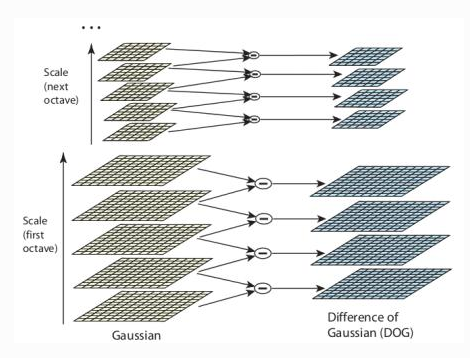
\includegraphics[width=0.5\textwidth]{UCT_MSc_Thesis/figs/sift_steps.png}
%----------------------------------------------------
    \caption[SIFT Difference of Gaussian]{Shown on the left are scale-space images produced by convolving the initial image with Gaussians repeatedly for each octave. The difference-of-Gaussian (DoG) images on the right are produced by subtracting adjacent Gaussian images. The Gaussian image is down-sampled by two after each octave, and then the process is repeated. Taken from \cite{Lowe2004}.}
%----------------------------------------------------
    \label{fig:sift_steps}
\end{figure}
%....................................................

\textbf{Speed up Robust Feature (SURF)} is the feature detector technique, which is an approximation of SIFT. The algorithm performs fast computation operations using box filters, thus enabling real-time applications such as object recognition \cite{BAY2008346}. SURF approximates the LoG with box filters, the advantage being that convolution with box filter can be easily calculated with the assistance of image integrals. Squares are used for approximation instead of Gaussian averaging because convolution with a square is faster than an image's integral. Furthermore, the estimation can be performed in parallel, the following Figure \ref{fig:surf_approximation} shows such an approximation. 

%....................................................
\begin{figure}[H]
%----------------------------------------------------
    \centering
%----------------------------------------------------
    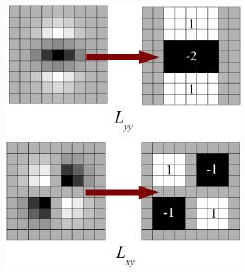
\includegraphics[width=0.5\textwidth]{UCT_MSc_Thesis/figs/surf_approximation.png}
%----------------------------------------------------
    \caption[Laplacian of Gaussian (LoG)]{Approximation of Laplacian of Gaussian (LoG) with Box Filter, where the grey regions are equal to zero.  Taken from \cite{BAY2008346}.}
%----------------------------------------------------
    \label{fig:surf_approximation}
\end{figure}
%....................................................

SURF relies on the determinant of the Hessian matrix for both scale and location of key-points. To find the key-points' orientation, SURF uses wavelets responses in both horizontal and vertical directions for a neighbourhood of size 6s and then applying Gaussian weights. They are then plotted as shown in Figure \ref{fig:surf_orientation}, where the red arrow is the dominant orientation, computed by summing of all the responses within a sliding orientation window. 

%....................................................
\begin{figure}[H]
    \centering
%----------------------------------------------------
    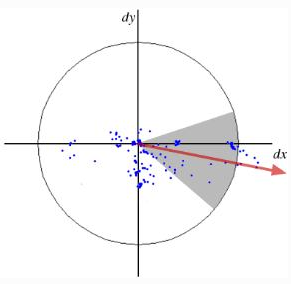
\includegraphics[width=0.5\textwidth]{UCT_MSc_Thesis/figs/surf_orientation.png}
%----------------------------------------------------
    \caption[Surf wavelet responses]{SURF uses wavelets responses in both horizontal and vertical directions then applying Gaussian weights, where the red arrow is the dominate orientation, computed by summing of all the responses within a sliding orientation window. Taken from \cite{BAY2008346}.}
%----------------------------------------------------
    \label{fig:surf_orientation}
%----------------------------------------------------
\end{figure}
%....................................................

Feature descriptor is achieved by again using wavelet responses in horizontal and vertical direction around a neighbourhood of size 20$\times$20 around the key-point, which is then divided into sub-regions of size 4$\times
$4 and then for each sub-region the wavelet responses are taken and represented to get SURF feature descriptor. SURF allows faster matching by using the sign of the Laplacian which is already computed by the detection, the sign distinguishes bright blobs on a dark background, which in case of matching the features are compared if they have matching contrast.

\textbf{Oriented FAST and Rotated BRIEF (ORB)} was developed at OpenCV labs as an alternative to SIFT and SURF. ORB fuses the well-known Features from Accelerated and Segments Test (FAST) key-point detector and BRIEF descriptor with modification to enhance performance \cite{Rublee2011}. 

FAST key-points are identified by comparing the brightness of 16 pixels surrounding a specific pixel, $p$. The pixels are then sorted into three categories lighter than $p$, darker than $p$ or similar to $p$. If more than eight of surrounding pixels are darker or brighter than $p$, then $p$ is selected as a key-point. Therefore, FAST key-points determine edges in the image. FAST key-point is, however, not an orientation and scale-invariant.

Similarly to SIFT, ORB identifies features at multiple scales, by using pyramids and representing the image at multiple scales. Change in intensity around the key-point is used to identify the orientation of the key-point. The intensity weighted centroid of the patch with located key-point (edge) at centroid is computed, to detect the change in intensity. The vector from the edge to centroid gives the orientation.

To compute the BRIEF descriptor, the algorithm takes all the key-points already found and converts them in binary feature vectors. In BRIEF, each key-point descriptor is defined by a feature 128 dimension vector, which as a floating-point number is 512 bytes. To prevent sensitivity to high-frequency noise, BRIEF begins by smoothing the image using a Gaussian kernel. Followed by selecting a pair of pixels in a defined neighbourhood of some height and width around the key-point. The first pixel is randomly selected from a Gaussian distribution centred around the key-point. Then the second on is randomly selected from a Gaussian distribution centred around the first pixel. If the first pixel is brighter than the second, a one is assigned else a zero. For a 128 dimension vector, this process is repeated 128 times, for each key-point. Given that BRIEF is not orientation invariant, ORB employs Rotation-aware BRIEF, by ``steering'' BRIEF descriptor in the key-point direction.

SIFT, SURF and ORB describe a feature with a key-point and a descriptor. In the next section, matching these features from images with partial overlap is discussed, followed by merging the images.

%====================================================
\subsection{Image matching}
%----------------------------------------------------

The features detected in the map images need to be matched with high accuracy to get the best transformation (scaling, translation and rotation). The features are matched from one map to another using either a Brute-Force matcher or Fast Library for Approximate Nearest Neighbors (FLANN) Matcher provided by OpenCV. Brute-Force matcher uses the distance between features of the map to another and finds the closest one. Different distance measurements can be used with this matcher, depending on the feature detector. It is recommended to use the Euclidean distance for SIFT and SURF, and Hamming distance binary string based descriptors such as ORB, BRIEF and BRISK \footnote{https://opencv-python-tutroals.readthedocs.io/en/latest/py\_tutorials/py\_feature2d/py\_matcher/py\_matcher.html}. FLANN stands for Fast Library for Approximate Nearest Neighbours, and it is optimised for large datasets and high dimensional features. However, FLANN Matcher is not necessary for this application.

%====================================================
\subsection{Matching features}
%----------------------------------------------------

Brute-Force Matcher is used to matching features between two different images. Given that features (key-points and descriptors) have been identified, Brute-Force Matcher takes descriptors from each image and matches them using a distance calculation to determine the closest feature.

Different distance calculations can be using, euclidean distance is recommended for SIFT and SURF, and hamming distance is recommended for ORB \cite{itseez2015opencv}.

Euclidean distance is defined as the absolute value distance between two coordinates and is described as:

%....................................................
\begin{equation}
%----------------------------------------------------
    d(p,q) = \sqrt{(p - q)^2}
%----------------------------------------------------
\label{eq:euclidean_distance}
\end{equation}
%....................................................

Where, $p, q$ are two coordinates on a line. 

On the other hand, Hamming distance is a metric for comparing binary data strings. As discussed in the previous section, ORB produces binary descriptors, which are compared with an XOR operation. After XORing the two values, the total number of 1s is counted, which is the Hamming distance. The smaller the number of 1s, the smaller the Hamming distance.

%====================================================
\subsection{Map alignment}
%----------------------------------------------------
\label{subsec:map_alignment}

Even though maps may have a large number of matches between them, there will be outliers present. These outliers can cause some possible errors while aligning, which may affect the result. 

To remove outliers, algorithms such as Random sample consensus (RANSAC) or LEAST\_MEDIAN (LMEDS) are used so that good matches which provide correct estimation can be used. These good matches are called inliers, and remaining outliers are removed. OpenCV's \textbf{estimateAffinePartial2D()} has been used to remove outliers and estimate the transformation matrix $T_{t_x, t_y, \theta}$, defined by Equation \ref{eq:transformation} earlier.

This method (\textbf{estimateAffinePartial2D()}) has the following parameters:
%....................................................
\begin{itemize}
%----------------------------------------------------
\item \textbf{method}:	Robust method used to compute transformation. The following methods are possible, RANSAC and LMEDS.
%----------------------------------------------------
\item \textbf{ransacReprojThreshold}:  Maximum re-projection error in the RANSAC algorithm to consider a point as an inlier.
%----------------------------------------------------
\item \textbf{maxIters}: The maximum number of robust method iterations.
%----------------------------------------------------
\item \textbf{confidence}: Confidence level, between 0 and 1, for the estimated transformation.
%----------------------------------------------------
\end{itemize}
%....................................................

RANSAC was used, RANSAC is a robust estimation iterative procedure that uses a minimal set of randomly sampled correspondences to estimate image transformation parameters, and finds a solution that has the best consensus with the data \cite{Fischler1981}. The parameter value of confidence has been selected to be $0.99$ to achieve high accuracy and $ransacReprojThreshold$, and $maxIters$ will be discussed later.

The transformation $T$ from Equation \ref{eq:transformation}, can now be used to align the one image to match the other. An affine transformation fixed to rotation, translation and scaling transformations is used. Affine transformations can also do the following transformation: identity, reflection and shear but these do not apply to this thesis.

%\subsection{Merging}

%To remove the uncertainty of the estimated to transformation, known information from the map metadata is used. Each Occupancy Grid in the Robotic Operating System (ROS) has the metadata presented in Figure \ref{fig:metadata}. The resolution of each map can determine the scaling factor expected from $T$ if the scaling factors match the transformation is deemed successful, and the maps are then merged.

%\begin{figure}[H]
%    \centering
%    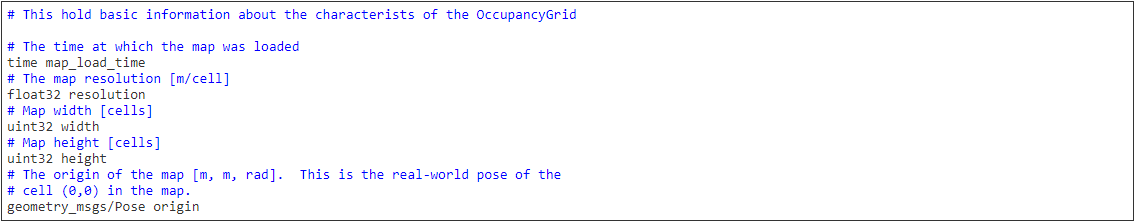
\includegraphics[width=1\textwidth]{figs/metadata_information.png}
%    \caption[Occupancy grid Metadata ROS Message]{Occupancy grid Metadata ROS Message, which is received with each %occupancy grid Map.}
%    \label{fig:metadata}
%\end{figure}


%\begin{figure}[H]
%   \centering
%    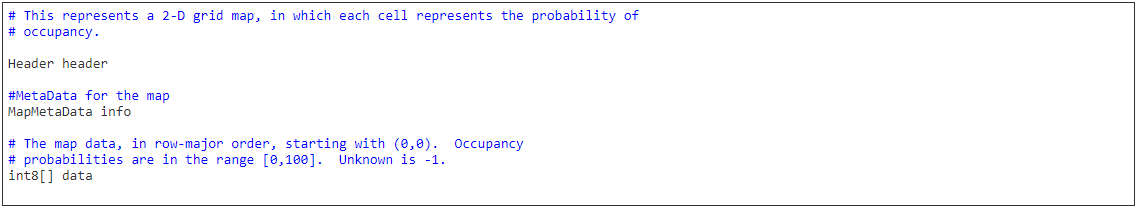
\includegraphics[width=1\textwidth]{figs/occupancy_grid_information.png}
%    \caption[Occupancy grid ROS Message]{Occupancy grid ROS Message, where data is an array describing the map and mapMetaData being the information about the map shown in Figure \ref{fig:metadata}}
%    \label{fig:occupancygridmsg}
%\end{figure}

%====================================================
\subsection{Method selection}
%----------------------------------------------------
\label{sub:sec:method}

Paper \cite{Karami2015}, investigates the sensitivity of SIFT, SURF, and ORB against intensity, rotation, scaling, shearing, fish-eye distortion, and noise. The investigation is general, and in the case of the work done in this thesis, further investigation is required for occupancy grid maps. This section investigates SIFT, SURF, and ORB's sensitivity against each rotation, scaling, translation, and noise, not includes in shearing and fish-eye distortion, which are not of interest in 2D occupancy grid maps, due to how they are generated. Open Source Computer Vision Library (OpenCV) \footnote{http://opencv.org}, which is an open-source BSD-licensed library that includes several hundred computer vision algorithms, is used for the image registration in this thesis.

In Figure \ref{fig:maps} are the maps used to test the robustness of the feature detection methods. These maps were produced in a real-world environment at the University of Cape Town due to work done in this thesis\footnote{Data-sets: \url{https://drive.google.com/drive/folders/1c\_2-T8FcrSmE0VDyHw20-jRLHKRuAvpE}}\footnote{GitHub repository: \url{https://github.com/dikokob/DikokoMScEng}}. The maps were produced using Hector-SLAM which each robot will be equipped with, and these maps are partial maps of the same area. The data used is later discussed in Chapter \ref{ch:experimental}.

%....................................................
\begin{figure}[H]
%----------------------------------------------------
    \centering
%----------------------------------------------------
    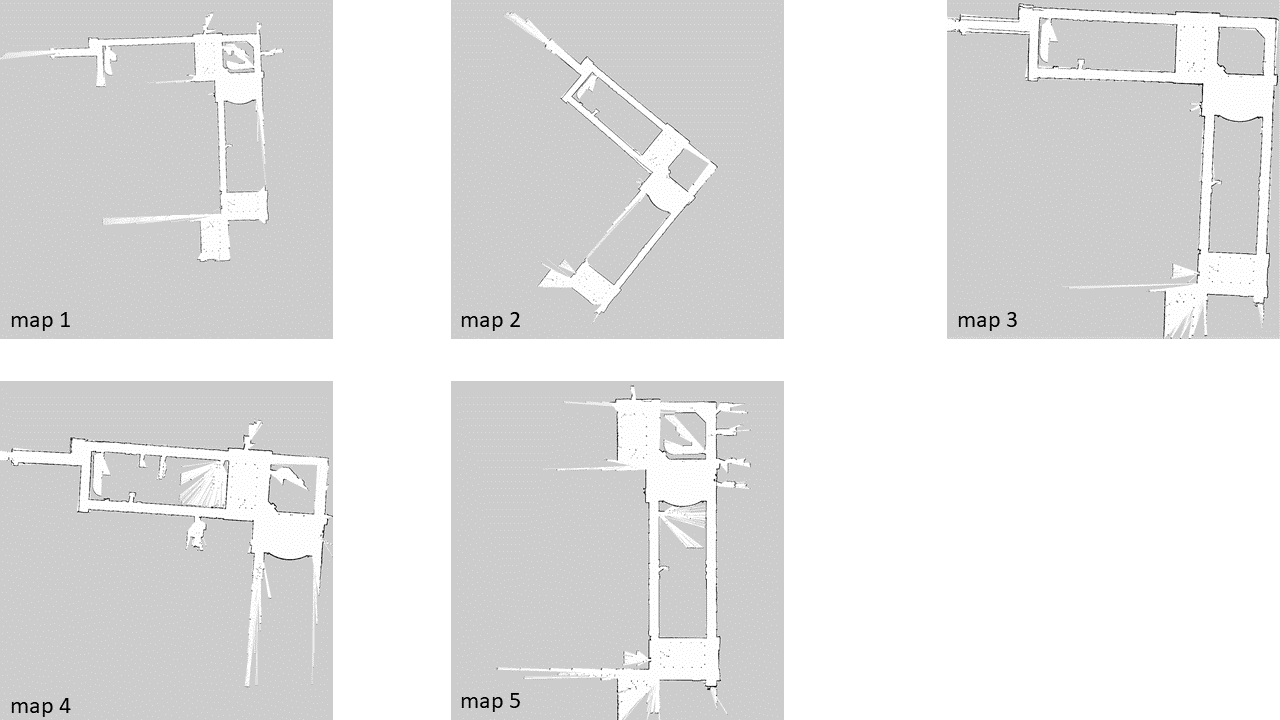
\includegraphics[width=1\textwidth]{figs/feature_images.png}
%----------------------------------------------------
    \caption[Occupancy grid map examples of a large indoor environment]{The following maps are of a large indoor environment used to test the robustness of the feature detection methods. The maps are produced using hector slam with a resolution of 0.5 m/cell. The generation of the maps are discussed in further details in Chapter \ref{ch:experimental}.}
%----------------------------------------------------
    \label{fig:maps}
%----------------------------------------------------
\end{figure}
%....................................................

A match ratio is used to investigate rotation, translation, scaling and noise sensitivity. The match ratio is calculated by

%....................................................
\begin{equation}
%----------------------------------------------------
    \frac{matches}{\min(num\_features\_orignal, num\_features\_mod)}
%----------------------------------------------------
    \label{eg:nmatch_ratio}
%----------------------------------------------------
\end{equation}
%....................................................

Where $num\_features$ is the number of features, and $matches$ is the number of matches found between the original and modified map features, using the earlier discussed Brute-Force matcher. The higher the match ratio, the more matches were found between the two maps. Note that in the investigations \textit{Kpnts1} are key-points from the original map and \textit{Kpnts2} are key-points from the modified map.

%====================================================
\subsubsection{Number of features}
%----------------------------------------------------

SIFT, SURF and ORB each produce a certain amount of features based on the algorithms. Figure \ref{fig:featuremaps} shows the features with descriptors shown by the feature's size and direction by the line within the circle. SIFT and ORB have a similar number of features whereas SURF has almost ten times more features, shown in \ref{table:numfeatures}. The number of features detected impacts the time cost of the process, more specifically the matching process. Also to be noted in Figure \ref{fig:featuremaps}, most of the ORB features are on the corners due to the nature of the algorithm and SIFT, and SURF features are highly variable size and location.

%....................................................
\begin{figure}[H]
%----------------------------------------------------
    \centering
%----------------------------------------------------
    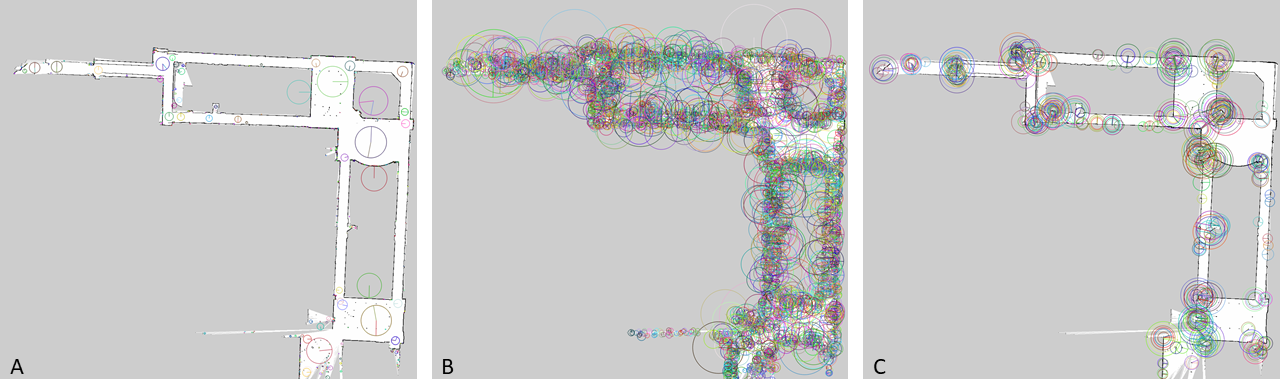
\includegraphics[width=1\textwidth]{figs/feature_maps.png}
%----------------------------------------------------
    \caption[Features detected on map3]{Features detected on $map_3$ from Figure \ref{fig:maps} where A) SIFT, B) SURF and C) ORB. See \footnote{https://github.com/dikokob/DikokoMScEng} for raw data. }
%----------------------------------------------------
    \label{fig:featuremaps}
%----------------------------------------------------
\end{figure}
%....................................................

%....................................................
\begin{table}[H]
%----------------------------------------------------
\centering
\caption{Average number of detected features (SIFT, SURF and ORB) of maps 1-5 in Figure \ref{fig:maps}.}
%----------------------------------------------------
%----------------------------------------------------
\begin{tabular}{ | m{3em} | m{2cm} | m{1.5cm} | m{1.5cm} | m{1.5cm} | m{3cm} | } 
%----------------------------------------------------
\hline
%----------------------------------------------------
\textbf{Maps} & \textbf{ORB}  & \textbf{SIFT} & \textbf{SURF} & \textbf{Total}\\ 
%----------------------------------------------------
\hline
%----------------------------------------------------
\textbf{map 1}  & 501 & 492 & 4291 & 5284 \\ 
%----------------------------------------------------
\hline
%----------------------------------------------------
\textbf{map 2}  & 500 & 528 & 3786 & 4814 \\ 
%----------------------------------------------------
\hline
%----------------------------------------------------
\textbf{map 3}  & 500 & 530 & 4503 & 5533 \\ 
%----------------------------------------------------
\hline 
%----------------------------------------------------
\textbf{map 4}  & 500 & 505 & 4224 & 5229 \\ 
%----------------------------------------------------
\hline 
%----------------------------------------------------
\textbf{map 5}  & 500 & 539 & 3282 & 4321 \\ 
%----------------------------------------------------
\hline 
%----------------------------------------------------
\end{tabular}
%----------------------------------------------------
\label{table:numfeatures}
%----------------------------------------------------
\end{table}
%....................................................

%\begin{figure}[H]
%    \centering
%    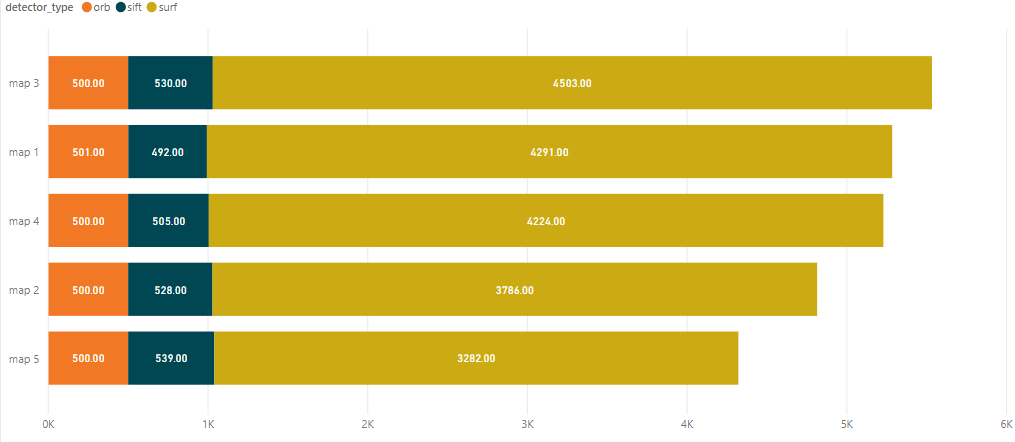
\includegraphics[width=1\textwidth]{figs/Number_of_Features.png}
%    \caption[Average number of features detected on each map using SIFT, SURF and ORB]{Average Number of Features detected on $map_{1-5}$ using different SURF, SIFT and ORB detection methods. }
%    \label{fig:numfeatures}
%\end{figure}

%====================================================
\subsubsection{Rotation}
%----------------------------------------------------

In this investigation, $map_3$ is rotated in steps of 30 degrees. The rotated map is matched with the original map. The results are shown in Figure \ref{fig:rotation} and Table \ref{table:rotation} are of $map_3$ rotated, where ORB is the fastest, followed by SIFT and SURF being the slowest. SIFT also has the highest match ratio, followed by ORB, with the lowest match ratio.

Table \ref{table:rotationangle} shows the match ratio versus the rotation angle, where rotation 0, 90 and 180 degrees ORB and SURF have the highest match ratio. However, they do not perform as well for other angles. The best overall performing feature detector is SIFT with an average of 0.90 match ratio, with SURF being the worst-performing. Also to be noted is that angles 0, 90 and 180 performed the best overall.

%....................................................
\begin{figure}[H]
%----------------------------------------------------
    \centering
%----------------------------------------------------
    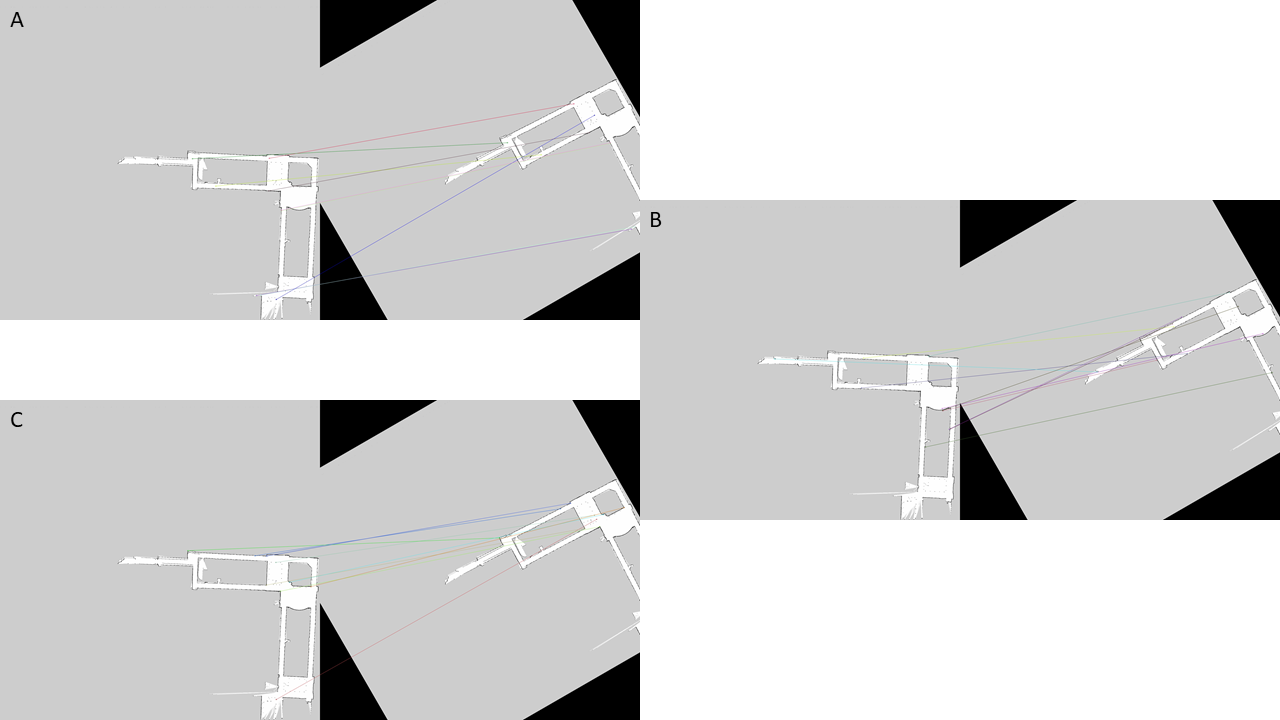
\includegraphics[width=1\textwidth]{figs/matching_of_30_rotation.png}
%----------------------------------------------------
    \caption{ The matching of 30$^\circ$ rotation images using (a) SIFT (b) SURF(c) ORB.}
%----------------------------------------------------
    \label{fig:rotation}
%----------------------------------------------------
\end{figure}
%....................................................

%....................................................
\begin{table}[H]
\centering
\caption{Results of comparing the images with 30$^\circ$ rotation.}
\begin{tabular}{ | m{3em} | m{2cm} | m{1.5cm} | m{1.5cm} | m{1.5cm} | m{3cm} | } 
\hline
& \textbf{Time(sec)} & \textbf{Kpnts1}  & \textbf{Kpnts2} & \textbf{Good Matches} & \textbf{Match Ratio}\\ 
\hline
\textbf{SIFT}  & 1.4 & 530 & 489 & 305 & 0.62\\ 
\hline
\textbf{SURF}  & 1.2 & 4503 & 5128 & 1370 & 0.30\\ 
\hline
\textbf{ORB}  & 0.39 & 500 & 500 & 280 & 0.56\\ 
\hline 
\end{tabular}
\label{table:rotation}
\end{table}


\begin{table}[H]
\centering
\caption{Matching ratio versus the rotation angle.}
\begin{tabular}{ | m{5em} | m{1cm} | m{1cm} | m{1cm} | m{1cm} | m{1cm} | m{1cm} | m{1cm} || m{1.6cm} | } 
\hline
\textbf{Angle $\rightarrow$} & \textbf{0$^\circ$} & \textbf{30$^\circ$} & \textbf{60$^\circ$} & \textbf{90$^\circ$} & \textbf{120$^\circ$} & \textbf{150$^\circ$} & \textbf{180$^\circ$} & \textbf{Average}  \\ 
\hline
\textbf{SURF} & 1 & 0.30 & 0.30 & 1 & 0.30 & 0.30 & 1 & 0.60 \\
\hline
\textbf{SIFT} & 0.95 & 0.62 & 0.63 & 0.92 & 0.63 & 0.65 & 0.90 & 0.90\\ 
\hline
\textbf{ORB} & 1 & 0.56 & 0.58 & 1 & 0.56 & 0.58 & 1 & 0.75 \\ 
\hline
\hline
%\textbf{Average} & 0.98 & 0.50 & 0.51 & 0.97 & 0.50 & 0.51 & 0.97 & 0.71 \\ 
%\hline
\end{tabular}
\label{table:rotationangle}
\end{table}

\subsubsection{Translation}
\label{sub:sec:translation}

In this investigation, $map_3$ is translated in steps of 200, with 0 being the control. The translated map is matched with the original map. The results are shown by Figure \ref{fig:translation}, Table \ref{table:translation} and Table \ref{table:translationchange}.

Table \ref{table:translation} shows that ORB is the fastest performing method followed by SIFT, and then SURF. Table \ref{table:translationchange}, shows that SURF as best performing method at match ratio of 0.99 followed closely by SIFT at 0.97. ORB has the lowest performance to varying translations, with a match ratio of 0.59.

\begin{figure}[H]
    \centering
    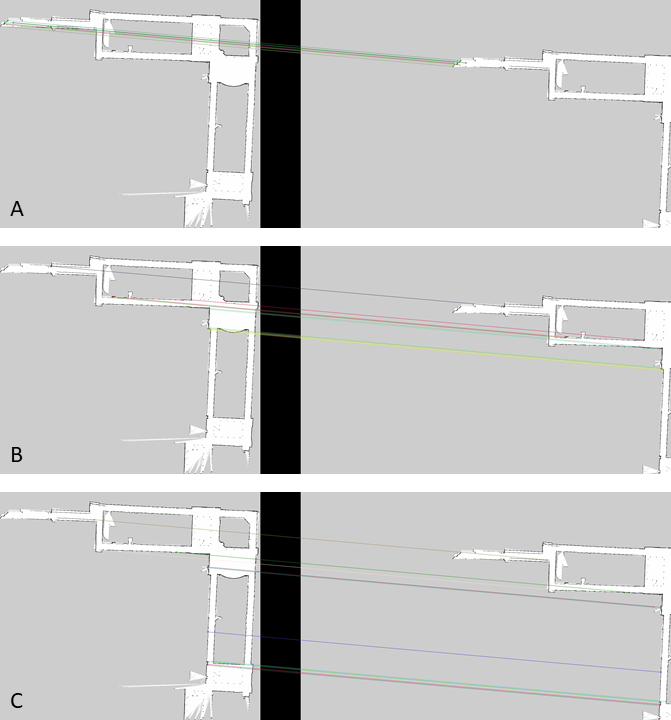
\includegraphics[width=1\textwidth]{figs/The_matching_of_translation_200.png}
    \caption{ The matching of translation(x:200 y:200) images using (a) SIFT (b) SURF (c) ORB.}
    \label{fig:translation}
\end{figure}

\begin{table}[H]
\centering
\caption{Results of comparing the images of translation in \ref{fig:translation}.}
\begin{tabular}{ | m{3em} | m{2cm} | m{1.5cm} | m{1.5cm} | m{1.5cm} | m{3cm} | } 
\hline
& \textbf{Time(sec)} & \textbf{Kpnts1}  & \textbf{Kpnts2} & \textbf{Good Matches} & \textbf{Match Ratio}\\ 
\hline
\textbf{SIFT}  & 3.23 & 530 & 285 & 278 & 0.98\\ 
\hline
\textbf{SURF}  & 3.79 & 4503 & 2598 & 2595 & 1\\ 
\hline
\textbf{ORB}  & 1.70 & 500 & 500 & 280 & 0.56\\ 
\hline
\end{tabular}
\label{table:translation}
\end{table}


\begin{table}[H]
\centering
\caption{Matching ratio versus the translation.}
\begin{tabular}{ | m{5.5em} | m{1cm} | m{1cm} | m{1cm} | m{1cm} | m{1cm} | m{1cm} || m{1.5cm} | m{1cm} | m{1cm} | m{1cm} | } 
\hline
\textbf{Translation $\rightarrow$} & \textbf{x:0 y:0} & \textbf{x:100 y:100}  & \textbf{x:300 y:300}  & \textbf{x:500 y:500} & \textbf{x:700 y:700} & \textbf{x:900 y:900} & \textbf{Average}   \\ 
\hline
\textbf{SIFT}  & 0.95 & 0.95 & 0.99 & 0.98 & 0.99 & 0.97 & 0.97 \\ 
\hline
\textbf{SURF}  & 1 & 0.99 & 0.99 & 0.99 & 0.99 & 0.99 & 0.99 \\ 
\hline
\textbf{ORB}  & 1 & 0.66 & 0.52 & 0.49 & 0.47 & 0.41 & 0.59 \\ 
\hline
\hline
%\textbf{Average}  & 0.98 & 0.87 & 0.83 & 0.82 & 0.82 & 0.79 & 0.85 \\ 
%\hline
\end{tabular}
\label{table:translationchange}
\end{table}


\subsubsection{Scaling}

In this investigation, $map_3$ is scaled in steps of 0.2. The scaled map is matched with the original map. The results are shown by Figure \ref{fig:scaling}, Table \ref{table:scaling} and Table \ref{table:scalingchange}. 

Table \ref{table:scaling} shows that for a scaling operation of 0.4, ORB is the fastest followed by SIFT then SURF. Furthermore, SIFT has the highest match ratio of 0.88 at a scale of 0.4, followed by SURF, then ORB.

Now Table \ref{table:scalingchange}, show the match ratio at multiple scales, which presents SIFT at the best overall performing method, with a match ratio of 0.82. Followed by SURF at 0.67, then ORB at 0.49.


\begin{figure}[H]
    \centering
    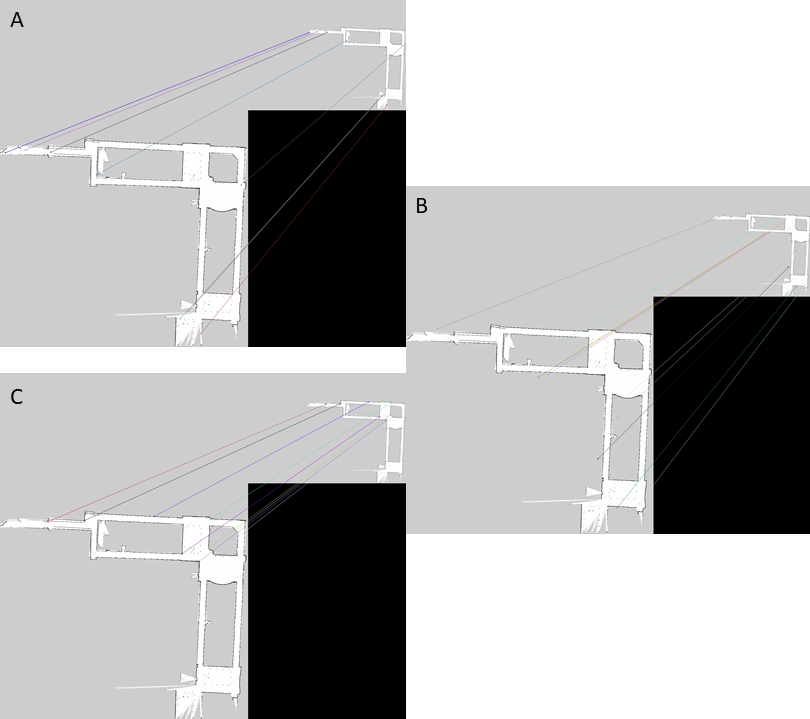
\includegraphics[width=1\textwidth]{figs/The_matching_of_scale_0_4.png}
    \caption{ The matching of varying scaling images using (a) SIFT (b) SURF (c) ORB.}
    \label{fig:scaling}
\end{figure}

\begin{table}[H]
\centering
\caption{Results of comparing the images with 0.4 scaling.}
\begin{tabular}{ | m{3em} | m{2cm} | m{1.5cm} | m{1.5cm} | m{1.5cm} | m{3cm} | } 
\hline
& \textbf{Time(sec)} & \textbf{Kpnts1}  & \textbf{Kpnts2} & \textbf{Good Matches} & \textbf{Match Ratio}\\ 
\hline
SIFT  & 1.05 & 530 & 84 & 74 & 0.88\\ 
\hline
SURF  & 1.35 & 4503 & 1013 & 671 & 0.66\\ 
\hline
ORB  & 0.29 & 500 & 496 & 208 & 0.42\\ 
\hline
\end{tabular}
\label{table:scaling}
\end{table}


\begin{table}[H]
\centering
\caption{Matching ratio versus the scaling.}
\begin{tabular}{ | m{5em} | m{1cm} | m{1cm} | m{1cm} | m{1cm} | m{1.5cm} | } 
\hline
\textbf{Scaling $\rightarrow$} & \textbf{0.2} & \textbf{0.4} & \textbf{0.6} & \textbf{0.8} & \textbf{Average} \\ 
\hline
\textbf{SIFT}  & 0.81 & 0.88 & 0.85 & 0.76 & 0.82 \\ 
\hline
\textbf{SURF}  & 0.68 & 0.66 & 0.67 & 0.66 & 0.67 \\ 
\hline
\textbf{ORB}  & 0.39 & 0.42 & 0.52 & 0.65 & 0.49 \\ 
\hline
\hline
%\textbf{Average}  & 0.62 & 0.65 & 0.68 & 0.69 & 0.66 \\
%\hline
\end{tabular}
\label{table:scalingchange}
\end{table}

\subsubsection{Noisy maps}
In this investigation, $map_3$ has salt and pepper noise applied at steps of 0.01. The modified image is then matched with the original image. The results are shown by Figure \ref{fig:noise}, Table \ref{table:noise} and table\ref{table:noisechange}. 

Table \ref{table:noise} shows match ratio and computation time at 3$\%$ noise, where ORB has the fastest computation time at 4.82 seconds followed by SIFT at 7.92 seconds, and SURF at 35.02 seconds close to ten times that of ORB.

Now Table \ref{table:noise} shows the match ratio of the different methods at steps of 0.01 noise. SIFT is best performing with an average of 0.83 match ratio followed by ORB at a 0.67 match ratio, and then SURF at a 0.61 match ratio.

\begin{figure}[H]
    \centering
    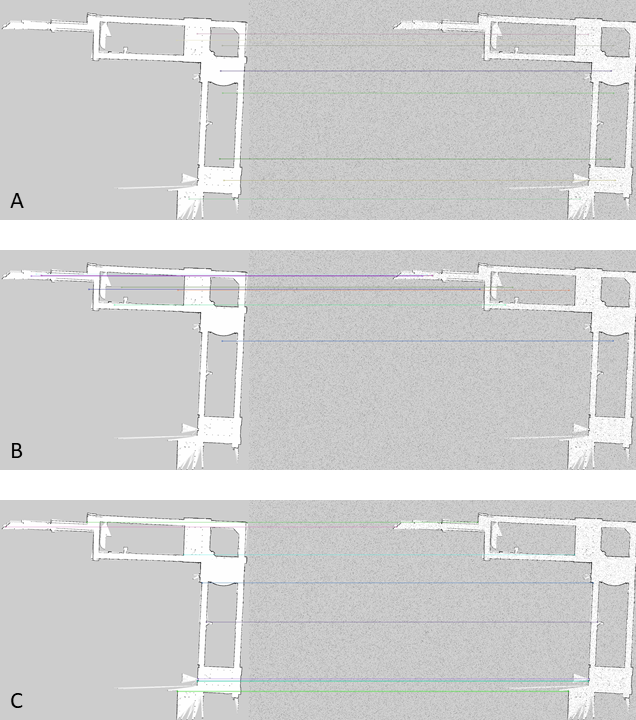
\includegraphics[width=1\textwidth]{figs/The_matching_of_noise_0_03.png}
    \caption{ The matching of 0.03 salt and pepper noise on varying images using (a) SIFT (b) SURF (c) ORB.}
    \label{fig:noise}
\end{figure}

\begin{table}[H]
\centering
\caption{Results of comparing the images with 0.03 salt and pepper noise.}
\begin{tabular}{ | m{3em} | m{2cm} | m{1.5cm} | m{1.5cm} | m{1.5cm} | m{3cm} | } 
\hline
& \textbf{Time(sec)} & \textbf{Kpnts1}  & \textbf{Kpnts2} & \textbf{Good Matches} & \textbf{Match Ratio}\\ 
\hline
\textbf{SIFT}  & 7.92 & 530 & 13436 & 441 & 0.83\\ 
\hline
\textbf{SURF}  & 35.02 & 4503 & 115422 & 2105 & 0.47\\ 
\hline
\textbf{ORB}  & 4.82 & 500 & 500 & 311 & 0.62\\ 
\hline
\end{tabular}
\label{table:noise}
\end{table}


\begin{table}[H]
\centering
\caption{Matching ratio versus the noise.}
\begin{tabular}{ | m{5em} | m{1cm} | m{1cm} | m{1cm} | m{1cm} | m{1cm} | m{1cm} | m{1cm} | m{1cm} | m{1cm} | m{1cm} | } 
\hline
\textbf{Noise $\rightarrow$ }& \textbf{0.01} & \textbf{0.02} & \textbf{0.03} & \textbf{0.04} & \textbf{Average} \\ 
\hline
\textbf{SIFT}  & 0.82 & 0.82 & 0.83 & 0.83 & 0.83 \\ 
\hline
\textbf{SURF}  & 0.76 & 0.65 & 0.55 & 0.47 & 0.61 \\ 
\hline
\textbf{ORB}  & 0.74 & 0.67 & 0.63 & 0.62 & 0.67  \\ 
\hline
\hline
%\textbf{Average}  & 0.78 & 0.72 & 0.67 & 0.64 & 0.70  \\ 
%\hline
\end{tabular}
\label{table:noisechange}
\end{table}

%====================================================
\subsubsection{Method selection summary}
%----------------------------------------------------

In this section, three different feature detection methods are compared similarly to work done in \cite{Karami2015}, with different translation and deformation such as scaling, rotation, noise and translation. For purposes of the work in this thesis, these transformations were applied to an occupancy grid map produced for this work. The results present display matching evaluation parameters such as the number of key-points, match ratio and the execution time for each method. 

The results show that ORB is the fastest, while SIFT performs the best in most scenarios. For exceptional cases when rotation angle is in steps of 90 degrees ORB and SURF outperform SIFT, these results match those of \cite{Karami2015}. In translation operations, SIFT and SURF perform similarly. Unlike results in \cite{Karami2015} ORB and SIFT do not show similar performance in noisy maps. In noisy maps, SURF's execution time is close to ten times the performance of ORB. In conclusion, SIFT is the most consistent in producing match ratios larger 0.80 for all the transformations and deformations. Therefore, SIFT will be used in this thesis because it has superior accuracy, and the time cost is not too high compared to SURF and ORB.


%====================================================
\section{Summary}
%----------------------------------------------------

In this chapter, the map merging problem was firstly defined, followed by investigating the literature around map merging. From the literature, image registration modules are discussed. Finally, image registration feature detectors SIFT, SURF and ORB are investigated to find the optimal methods for application in this thesis. The investigation is conducted due to the lack of literature comparing the methods in an occupancy grid map merging application. In the next chapter implementation of multi-robot, multi-session and multi-resolution map merging is discussed and described.




%\section{Notation and definition}
%
%The maps are assumed to be a 2D occupancy grid map \(m\) which is a matrix of N x M. Given two maps \(m_1\) and \(m_2\), which are 2D occupancy grid maps. We need to find the relative transformation(rotation and translation) between the maps. Let 2x1 translation vector  \(T\)  and 2 x 2 rotation matrix \(R_{\theta}\) be:

%\begin{equation}
%R_{theta} =  \begin{bmatrix}
%\cos(\theta) & -\sin(\theta)  \\
%sin(\theta) & \cos(\theta)
%\end{bmatrix} ,T =  \begin{bmatrix}
%\delta_{x}  \\
%\delta_{y}
%\end{bmatrix} 
%\end{equation}.

%Assuming the task is to merge \(m_2\) into \(m_1\), the map merging objective is to find \(R\) and \(T\) such that the transformed \(m_2\) which is \(m_{2}^{'}\) , overlaps with \(m_1\). The following equation is a defines a verification index which is maximized according to transformation \(R\) and \(T\) : 

%\begin{equation}
%(R_\theta, T) = argmax V(m_1 , m_{2}^{'})
%\end{equation}.

%The criterion \(V(\cdot)\) is used to evaluate the map merging process, such as a similarity index in (Birk and Capin, 2006).









%(Howard, 2006) use to prove that it is essential to choose the best SLAM algorithm to solve the map merging problem











 % Map Merging
%\include{Robot_Hardware} % Robot Hardware
% !TeX spellcheck = en_GB
%****************************************************
%	CHAPTER  - Implementation
%****************************************************
\chapter{Implementation}
\label{ch:implementation}
This chapter provides a detailed description of each module used in the multi-robot multi-session system to generate a global map on each team's mobile robot. 

\section{Overview}

In this work, a multi-robot, multi-session map merging algorithm capable of merging maps of different resolutions, is presented. Each robot in the system can generate a local and global map, hence it is a distributed system. Hector SLAM is used to generate the local maps, which are inputs to the map merging algorithm that produces a global map. A map merging algorithm is presented. The implementation of the algorithm is then presented for real-time capability. The map merging algorithm has input maps from other robots in the network and previously mapped session, enabling the robot to deal with multiple session mapping. 

\section{Map merging algorithm}
\label{sec:map_merging_algorithm}

This section describes the map merging algorithm used in this thesis, which is based on image registration. The image registration is transforming different images into the same coordinate system, using the following steps feature detection, matching, alignment and merging. In this work, occupancy grid maps are represented as images where a pixel defines whether an area is occupied, unoccupied or unknown. These images can be taken at multiple resolutions, viewpoints, and using different sensors; therefore, the spatial relationships or the maps include rotation, translation and scaling. As described in the previous chapter Scale-invariant feature transform (SIFT) will be used as a feature detector as it deals well with the spatial relationship described above. 

OpenCV was started at Intel in 1999 by Gary Bradsky, however, the first release in 2000 when it was used on Stanley (the vehicle that won the DARPA Grand Challenge that year). OpenCV is supported in C++, Python and Java; hence it can be used across various systems. The Python API of OpenCV (OpenCV-Python) is used to implement the solution; the API includes a wide range of tools such as feature detection, object detection, machine learning and video analysis. The image registration module used in this work is based on Scale-invariant feature transform (SIFT), results presented in Chapter \ref{sec:map-merging} show that it is superior for this scenario. The scale and rotation invariant nature of SIFT, it can be used in multi-resolution scenarios.

Feature detection, matching features, and alignment are included and merging the maps to form a global map.

\subsection{Transformation}
Assume there are two maps $map_1$ and $map_2$, where $map_1$ is the local map of $robot_1$ and consequently $map_2$ is the local map of $robot_2$. This section describes the process of transforming $map_2$ into $map_1$'s frame of reference. Algorithm \ref{alg:1} describes this process.

\begin{algorithm}
\SetAlgoLined
\SetNoFillComment
\DontPrintSemicolon

\tcc{This function transforms $map_2$ into $map_1$'s frame. The function requires two 2D occupancy grid maps of size n by m and RANSAC parameters(confidence, and reproj\_threshold)}


\SetKwProg{Fn}{Function}{}{end}

\Fn{Transform($map_1, map_2, confidence, reproj\_threshold$) : $transformed\_map_2, scale$}{

\tcc{extract feature key-points and corresponding descriptors}
$kp_1$, $des_1$ = detect\_keypoint\_descriptors($map_1$) \;

$kp_2$, $des_2$ = detect\_keypoint\_descriptors($map_2$) \;

\tcc{extract feature matches between two maps}
good\_matches = match\_features($des_1$, $des_2$) \;

\tcc{get feature locations of good matches}
$feature\_locations_1$ = [0, good\_matches.length][0, 2] : 2D array of float \;
$feature\_locations_2$ = [0, good\_matches.length][0, 2] : 2D array of float \;
        
\For{i, match in enumerate(good\_matches)} 
{ 
    $feature\_locations_1$[i, :] = $kp_1$[match.$des_1$\_index].pt \;
    $feature\_locations_2$[i, :] = $kp_2$[match.$des_2$\_index].pt \;
}
\EndFor

\tcc{compute match ratio}
$match\_ratio = good\_match.length/min(kp_1.length, kp_2.length)$ \;
\tcc{compute maximum iterations needed to estimate affine transformation matrix using RANSAC}
$max\_iter = \log(1-confidence)/\log(1-match\_ratio^2)$ \;

\tcc{estimate affine transformation matrix}
affine\_transformation\_matrix = estimate\_affine\_transformation($feature\_locations_1$, $feature\_locations_2$,  $max\_iter$, $confidence$, $reproj\_threshold$) \;

\tcc{transform map using affine transformation matrix}
$transformed\_map_2$ = affine\_transform($map_2$, affine\_transformation\_matrix) \;

\tcc{get scale and angle of rotation from the transformation matrix}
$ss$ = affine\_transformation\_matrix[0, 1] \;
$sc$ = affine\_transformation\_matrix[0, 0] \;
$scale = \sqrt{ss * ss + sc * sc}$\;
$angle\_of\_rotation = \arctan{\frac{ss}{sc}} * 180 / \pi$ \;


\Return $transformed\_map_2$, $scale$ \;
}
\caption{Transform map into main maps frame of reference}
\label{alg:1}
\end{algorithm}

Feature detection is the initial step described in lines 2-3 in algorithm \ref{alg:1}, where a pair of key-points and descriptors are returned (see Chapter \ref{sec:map-merging} for more information). The features are then matched using a Brute-Force Matcher (line 4). The Brute-Force Matcher takes descriptors from each image and matches them using a distance calculation to determine the closest features. In this case the Euclidean distance described by Equation \ref{eq:euclidean_distance} \cite{Lowe2004}. These matches are referred to as $good\_matches$. The $good\_matches$ are then used to get the locations of the features that were $good\_matches$ in lines 5-10. Next, the affine transformation matrix described by Equation \ref{eq:transformation} is computed using RANSAC. In Section\ref{subsec:map_alignment}, parameters $ransacReprojThreshold$ and $maxIters$ were introduced and here we define their values. 

\textbf{$maxIters$} is the maximum number of iterations and is described by the following equation :

\begin{equation}
    1-confidence = (1 - match\_ratio^{n})^{maxIters}
\end{equation}

where, $\{confidence | confidence \in \mathbb{R}, 0 < confidence < 1 \}$, $match\_ratio$ is the ratio of possible matches to good matches described by Equation \ref{eg:nmatch_ratio}, $n$ is the minimum number of features needed for a match \cite{Fischler1981}. By taking the $\log$ of both side get the following equation:

\begin{equation}
    maxIters = \frac{\log(1-confidence)}{ \log(1 - match\_ratio^{n})}.
\end{equation}

Then we choose a $confidence$ of $0.99$ which ensures minimal error, and minimum number of features $n$ of 2, to get:

\begin{equation}
    maxIters = \frac{\log(0.01)}{ \log(1 - match\_ratio^{2})}
\end{equation}


The maximum iterations can then be described by the following Figure \ref{fig:itervsmatch}. Where the smaller the match ratio, the more iterations are required to estimate the best model fit.
\begin{figure}[!h]
\centering
\begin{tikzpicture}

\begin{axis}[
    title={Number of iterations vs. match ratio},
    xlabel={Match ratio},
    ylabel={Number of iterations},
    domain=0:1, 
    samples=1000, 
    color=blue,
    ymajorgrids=true,
    xmajorgrids=true,
    grid style=dashed
]
\addplot[color=red]{-4.60517/(ln(1 - x) + ln(1 + x))};
\legend{$k = \frac{\ln(0.01)}{\ln(1 - match\_ratio^2)}$}
\end{axis}

\end{tikzpicture}
\caption{This figure illustrates the relationship between the number of iterations and the match ratio. The lower the match ratio, the higher the number of iterations. Therefore, lower match ratio matches are computationally costly compared to higher match ratio matches.}
\label{fig:itervsmatch}
\end{figure}

RANSAC uses $ransacReprojThreshold$ in order to determine if a data sample agrees with a model or not. The samples under this threshold will then form that consensus for that model and the data set's inliers if the correct model is found. Hence, it should be chosen according to the model needs. To determine the threshold for this thesis's work, maps in Figure \ref{fig:maps} are paired into groups of two giving a combination of 10. These where then run on line 1 - 14 of algorithm \ref{alg:1}. These maps were then merged and then recorded if the merge was successful if they failed. Table \ref{table:ransacReprojThreshold} shows that $ransacReprojThreshold$ values of 8,9 and 10 show a $100\%$ success rate this work we will use a $ransacReprojThreshold$ value of 9. 


\begin{table}[h]
\small
\setlength\tabcolsep{0.2pt}
\begin{longtable}{|p{2.1cm}|p{1.2cm} p{1.2cm} p{1.2cm} p{1.2cm} p{1.2cm} p{1.2cm} p{1.2cm} p{1.2cm} p{1.2cm} p{1.2cm}|p{2.2cm}|}%{|c|cccccccccc|c|}
\caption[Determining $ransacReprojThreshold$]{Results from running merging on threshold between 1 and 10 to determine the optimal $ransacReprojThreshold$. Where P represents a successful transformation and F a failed transformation.} 
\hline
\multirow{2}{*}{\textbf{Threshold}} & \multicolumn{10}{c|}{\textbf{Combination Num}}                                                    & \multirow{2}{*}{\textbf{P Rate (\%)}} \\ \cline{2-11}
            & 1       & 2       & 3       & 4       & 5       & 6       & 7       & 8       & 9       & 10  &    \\ 
\hline
\endfirsthead
\endhead
\hline
\endfoot
\endlastfoot

1                                   & F & F & P & P & F & P & F & P & P & F & 50                        \\
2                                   & F & F & P & P & F & P & F & P & P & P & 60                        \\
3                                   & P & P & P & P & P & P & F & P & P & P & 90                        \\
4                                   & P & P & P & P & P & P & P & P & F & P & 90                         \\
5                                   & P & P & P & P & P & P & P & P & F & P & 90                         \\
6                                   & P & P & P & P & P & P & P & P & F & P & 90                        \\
7                                   & P & P & P & P & P & P & P & P & F & P & 90                         \\
8                                   & P & P & P & P & P & P & P & P & P & P & 100                       \\
9                                   & P & P & P & P & P & P & P & P & P & P & 100                       \\
10                                  & P & P & P & P & P & P & P & P & P & P & 100                       \\ 
\hline
\label{table:ransacReprojThreshold}
\end{longtable}
\end{table}
Finally, from the affine transformation matrix, the scaling factor and angle of rotation are calculated to be used in further processes. The transformation matrix is of the form:

\begin{align}
M &=
\begin{bmatrix}
cos(\theta)\dot s &  -sin(\theta)\dot s & t_x\\
sin(\theta)\dot s &  cos(\theta)\dot s & t_y 
\end{bmatrix}
\label{eq:rotation-mat}
\end{align}
where, \(\theta\) is the rotation angle, \(s\) the scaling factor and $t_x$,$t_y$ are translations in \textit{x}, \textit{y} axes respectively.

The scaling factor ($s$) and rotation angle ($\theta$)) can be computed using:

\begin{equation}
\begin{split} 
s &=  \sqrt[2]{ M_{1,2}*M_{1,2} + M_{1,1}*M_{1,1} }  \\ 
\theta &= \arctan{(\frac{M_{1,2}}{M_{1,1}})} \times \frac{180}{\pi}
\label{eq:rotat_scale}
\end{split}
\end{equation}.


\subsection{Multiple map transformation}

The \textbf{Transformation} function (algorithm \ref{alg:2})is then used to compute and transform more than one map into the local map's frame of reference. The \textbf{Main} function (algorithm \ref{alg:2}) receives multiple maps and their corresponding resolutions, and then they are merged to form a global map.

\begin{algorithm}[H]
\SetAlgoLined
\SetNoFillComment
\DontPrintSemicolon

\tcc{This is the primary function which receivers all the maps and corresponding scales, then transforms them relative to map[0] and returns the $global\_map$}


\SetKwProg{Fn}{Function}{}{end}

\Fn{Main($maps\_list, map\_resolutions\_list$) : $global\_map$}{
\tcc{initialise variables}
$confidence$ = $0.99$ \;
$reproj\_threshold$ = $9$ \;
$successfully\_transformed\_maps$ = $[]$ \;

\tcc{Loop through maps and transform them relative to $maps\_list[0]$}
\For{$\ i\  in\  range(1, len(maps\_list$))} 
{ 
\tcc{transform map based on the reference $maps\_list[0]$}
$transformed\_map, scale= Transform(map_1, map_2, confidence, reproj\_threshold)$ \;

\tcc{check success of transformation based on resolution}
\If {$(map\_resolutions\_list[0] \times (1-confidence)) > abs(map\_resolutions\_list[0] - (map\_resolutions\_list[i]/scale))$}
{
$successfully\_transformed\_maps.append(transformed\_map)$ \;
}

}

\EndFor

$global\_map = maps\_list[0]$ \;

\tcc{merge only successfully transformed maps}
\For{map in successfully\_transformed\_maps}
{
$global\_map = merge(global\_map, map)$\;
}

\Return $global\_map$\;
}
\caption{Main Function}
\label{alg:2}
\end{algorithm}

Given that not all transformations will be successful, the success is determined by comparing the expected scaling factor and the computed scaling factor. The expected scaling factor is determined by the local map's resolution divided by the resolution of maps from the other robot. This expected scaling factor needs to be within $1 - confidence$, which is the expected RANSAC estimation error. The successful maps are then merged using the following rule in Table \ref{tab:merge-rule}, which allows for a suitable global map to be obtained. If there are one or more successful alignments the map is then returned with it is corresponding resolution.

\begin{table}[H]
\centering
\caption{Rules of Map Merging between two partial maps.}
\begin{tabular}{l|l|c|c|c|c}
\multicolumn{2}{c}{}&\multicolumn{2}{c}{Partial Map 2}\\
\cline{3-5}
\multicolumn{2}{c|}{}&\textbf{Unknown}&\textbf{Free}&\textbf{Occupied}\\
\cline{2-5}
\multirow{2}{*}{Partial Map 1}& \textbf{Unknown} & Unknown & Free & Occupied\\
\cline{2-5}
& \textbf{Free} & Free & Free & Occupied\\
\cline{2-5}
& \textbf{Occupied} & Occupied & Occupied & Occupied\\
\cline{2-5}
\end{tabular}
    
    \label{tab:merge-rule}
\end{table}


\section{ROS implementation}

The algorithm \ref{alg:2} described above is then implemented on the Robot Operating System (ROS) to perform the map merging algorithm in real-time. Figure \ref{fig:systemoverview} describes the system overview of a robot. The robot will receive maps from other robots, maps from previous sessions, and a local map that it produces onboard, and merge them to produce a global map. Each robot must scan the network for possible partial local maps from other robots, to retrieve the maps.

\begin{figure}[H]
    \centering
    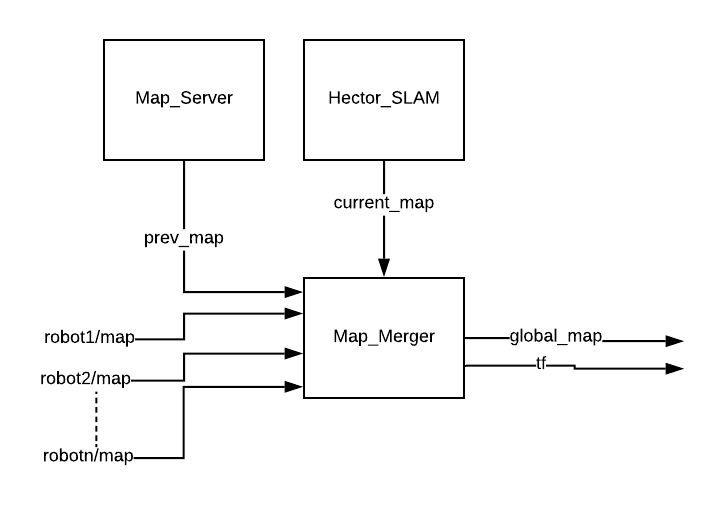
\includegraphics[width=1\textwidth]{figs/ROS_Block_Diagram_2.png}
    \caption{System overview of the solution. The map merging algorithm's inputs included the current partial map ($current\_map$), previous partial map ($prev\_map$), and partial maps of other robots in the environment ($robot1/map, $). The resultant map includes the global map ($global_map&)$ and transformations ($tf$).}
    \label{fig:systemoverview}
\end{figure}


Therefore, using ROS needs to solve the following problems:

\begin{itemize}
    \item \textbf{Communication} between robots
    \item \textbf{SLAM} implementation to produce a local map
    \item \textbf{Serve} maps from previous sessions
    \item \textbf{Map merging} algorithm needs to be incorporated and the resulting global map needs to be published
\end{itemize}


\subsection{What is ROS?}

Robot Operating System (ROS) is an open-source, meta-operating system used widely in robotics, and currently maintained by Open Robotics \footnote{https://www.openrobotics.org/}. ROS is designed to work with both physical and simulated robots and provides hardware abstraction, low-level device control, implementation of commonly-used functionality, message-passing between processes, and package management. The creators had a philosophy to \textit{"allow anyone to create functionalities that can be shared and used in other robots without much effort so that we do not reinvent the wheel"} \cite{Quigley2009}. For example, a driver for ROS to interact with an Arduino was created and shared with the ROS community. The community makes the framework easy to adopt for many users from Researchers to Hobbyists.


%\begin{figure}[H]
%    \centering
%    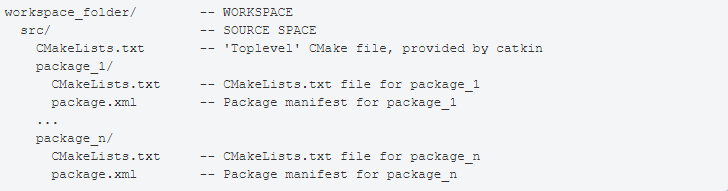
\includegraphics[width=0.8\textwidth]{figs/workspace_example.png}
%    \caption{A work-space in ROS Kinetic is referred to as catkin. This is an example catkin  work-space, showing multiple package %folder structure. The packages can be written in different programming languages(Python, C++, and Lisp, and has experimental %libraries in Java and Lua).}
%    \label{fig:ros-workspace}
%\end{figure}

ROS defines a recommended file structure and software build to promote reuse and ease of sharing in the community. ROS uses the concept of packages (similar to the UNIX operating systems) as the ROS ecosystem's fundamental building block. ROS currently supports the following programming languages Python, C++, and Lisp, and has experimental libraries in Java and Lua.

\subsection{ROS communication}

For the robots to communicate, ROS implements several different communication styles, including synchronous communication over services, asynchronous streaming of data over topics, and storage of data on a Parameter Server. The communication is facilitated by the peer-to-peer network, which can be distributed across machines. The network is based on a graph architecture with a decentralised topology where processing occurs in \textit{nodes} that may publish or subscribe messages, such as multiplex sensor, control, state, planning and actuators. Topics are asynchronous, and \textit{nodes} do not explicitly communicate with each other, services provide synchronous communication, as shown in Figure \ref{fig:ros-basic-concept}.

\begin{figure}[H]
    \centering
    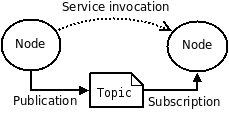
\includegraphics[width=0.4\textwidth]{figs/implementation/ROS_basic_concepts.png}
    \caption{This illustrates the basic node concept.Note that \textit{nodes} do not explicitly communicate with each other, services provide synchronous communication. Taken from \cite{Quigley2009}.}
    \label{fig:ros-basic-concept} 
\end{figure}

The ROS \textit{master} acts as a name-service for the graph; it stores topics and services information for ROS \textit{nodes}, as shown in Figure \ref{fig:ros-basic-concept}. \textit{Nodes} report information to the \textit{master}, and receive messages (include arbitrarily nested structures and arrays) from other \textit{nodes} through the \textit{master}. Nodes need to be registered to the \textit{master} to receive and pass messages. Messages (shown in Figure \ref{fig:ros-master-nodes}) are communicated via topics between \textit{nodes} using publish/subscribe architecture. A node subscribes to a topic, requests a connection through the \textit{master} and connects to a publisher node, hence receiving messages. There may be multiple concurrent \textit{nodes} publishing and subscribing to a single topic, and a node may publish and subscribe to multiple topics. The \textit{master} will also make callbacks to \textit{nodes} when registration information changes, which allows \textit{nodes} to create connections as new \textit{nodes} are registered dynamically. Bag files are used to save and playback ROS messages such as sensor data to develop and test algorithms.


\begin{figure}[H]
    \centering
    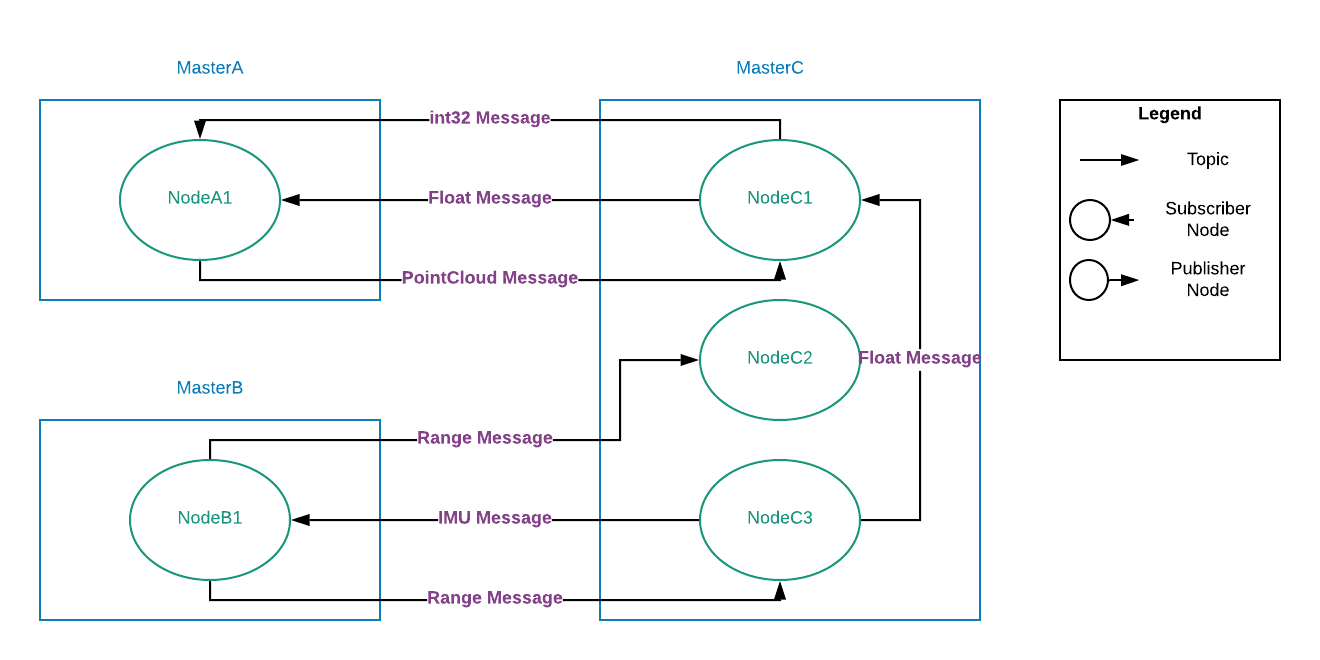
\includegraphics[width=0.9\textwidth]{figs/ros_master_nodes.png}
    \caption{An example of multiple machine/robot ROS implementation architecture. This shows the interaction of nodes between multiple machines/robots. Messages are passed through topics.}
    \label{fig:ros-master-nodes}
\end{figure}

%\begin{figure}[H]
%    \centering
%    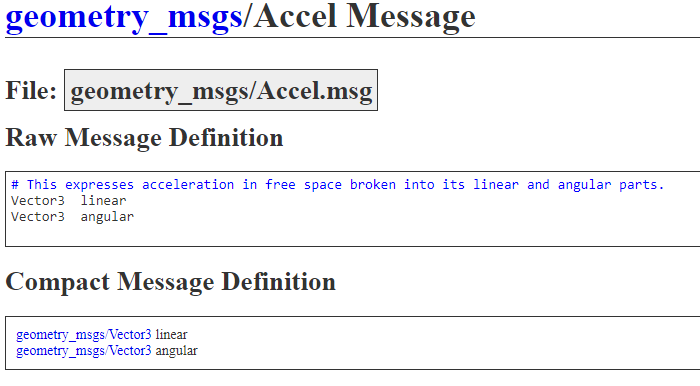
\includegraphics[width=0.7\textwidth]{figs/Ros_message_example.png}
%    \caption{This is an example of an \textit{Accel} message which is as message used to exchange, the linear %and angular vectors are in 3 axes(x, y, z).}
%    \label{fig:ros-message}
%\end{figure}


For example, given that there is a need to control and access data from a Hokuyo laser range-finder, \textit{hokuyo node} driver can be used to talk to the laser and publishes messages of the following type sensor \textit{msgs/LaserScan} to a topic named \textit{scan}. A node (i.e. \textit{laser process} ) can be written to subscribe to messages on the scan topic, to process \textit{msgs/LaserScan} messages. Note that all \textit{hokuyo node} does is to publish messages to the \textit{scan} topic, without knowledge of any nodes subscribed to the topic. On the other hand, the \textit{laser process} node subscribes to \textit{scan} the topic without knowledge of whether any node is publishing. Hence the nodes are decoupled, the nodes can be started, killed and restarted. 

When dealing with multiple robots,  there may be a  need to remap topics for each robot, primarily when robots used the same nodes internally.  ROS supports command-line remapping of names,  which means a compiled program can be reconfigured at run-time to operate in a different graph topology.  For example, the outputs from a laser range-finder for robot1 should not be published to the same topic as the outputs from the laser range-finder of robot2; therefore each robot should publish the scan message to different topics.  Defining a prefix will allow each robot to use a unique name-space for all data and transformations; for example, the two robots' laser scan topic will be robot0/scan, robot1/scan.

\subsection{SLAM in ROS}

Examples of ROS packages dedicated to SLAM algorithms include \(slam\_gmapping\)\footnote{http://wiki.ros.org/gmapping}, \(mrpt\_slam\)\footnote{http://wiki.ros.org/mrpt\_slam?distro=kinetic} and \(hector\_slam\)\footnote{http://wiki.ros.org/hector\_slam}. The stable and commonly used \textit{hector\_slam} is implemented in this work, due to the advantages discussed in Section\ref{sec:hector_slam}. The \textit{hector\_mapping} node is in the package, and it is a SLAM approach that can be implemented without odometry and platforms that exhibit roll/pitch motion(of the sensor, the platform or both) such as quad-rotor UAVs. It leverages the high update rate of modern LIDAR systems like the Hokuyo UTM-30LX and provides 2D pose estimates at the sensors' scan rate. While the algorithm does not provide explicit loop closing ability, it is sufficiently accurate for many real-world scenarios as described in \cite{Eliwa2017}. Furthermore, the system has successfully been used on unmanned ground robots, unmanned surface vehicles, handheld mapping devices and logged data from quad-rotor UAVs and was developed by \cite{Kohlbrecher2011a}.

\subsection{Map and pose exchange}

Robots must be aware of other teammates who join and leave the network, to perform the mapping task cooperatively.  This communication is achieved using a non-distributed \textit{roscore} which is a collection of nodes and programs of a ROS system.  Instead of running \textit{roscore} on each robot a dedicated robot or networked computer will be used to facilitate the communication, to do this \(\$roscore\) is run on the machine chosen to be the master, then the IP of the communication machine is used to run the following \(\$export ROSMASTERURI=http://masterrobotIP:1234/ \)on each robot in the network, to add them to the network.  Even though the master \textit{roscore} has been selected, nodes will still be computed on the individual robots,\textit{roscore} only facilities communication between the teammates.

Assuming that each robot is aware of its ID, i.e. robot1, the robot searches through topics to find which robots exist in the network.   Since robots can leave the network(i.e., map an area with low-quality network link), each robot maintains a list of all the mobile robots.   Assigning a  prefix allows robots to share information such as occupancy grids,  poses, laser scans or messages.  The following information is shared between the robots \textit{OccupancyGrid} and \textit{Pose}.

\subsection{Multi-session}

Multi-session mapping considers the problem of combining the results of mobile robot SLAM missions performed repeatedly over time in the same environment. The goal is to robustly combine multiple maps from different missions in the same environment in a standard coordinate system. Multi-session mapping involves having to deal with the fact that robots over long period missions eventually will be shut down and may revisit areas where they previously mapped. One way of doing multi-session mapping is having a robot localise it is self in a previously-built map. The solution allows the robot to use the same referential, and only one map is created per session; however, this requires the robot the start in the already mapped portion of the environment. In this work, the previously mapped portion of the environment is dealt with as a map from another robot. Hence the robot is not required to start in the portion of the environment previously mapped. Using ROS \(map\_server\), a map is stored and can be retrieved later for use in another process. After a session, the map is stored, and if a map were previously stored on startup, it would be fed into the map merging algorithm.

\subsection{ROS node}

Figure \ref{fig:ros-node-implementation} illustrated the ROS \textit{node} used in this work. The \textit{node} is implemented using Python, the \textit{rospy} library is used to interact with the ROS system. The \textit{node} is designed with parameters to alter the image registration process and parameters to alter the rate at which the \textit{node} runs. In step one the parameters are initialised to default values of which the image registration parameters are determined in Chapter \ref{sec:map-merging}, it is also necessary to know the current robot map topic. The current robot topic is used to ensure that all the partial maps are transformed into that frame. Step two involves getting the list of all the topics which are in the network using \textit{rospy.get\_published\_topics()}; the published topics messages of type \textit{nav\_msgs/OccupancyGrid} are then selected for the map merging process. In step 6 and 7, if there are maps in the network, the maps are then stored using the \textit{map\_server} \textit{node}. In the final step 8, the image registration based map merging algorithm is used. The map merging algorithm is described in Section\ref{sec:map_merging_algorithm}\footnote{GitHub repository: \url{https://github.com/dikokob/DikokoMScEng}}.

\begin{figure}[H]
    \centering
    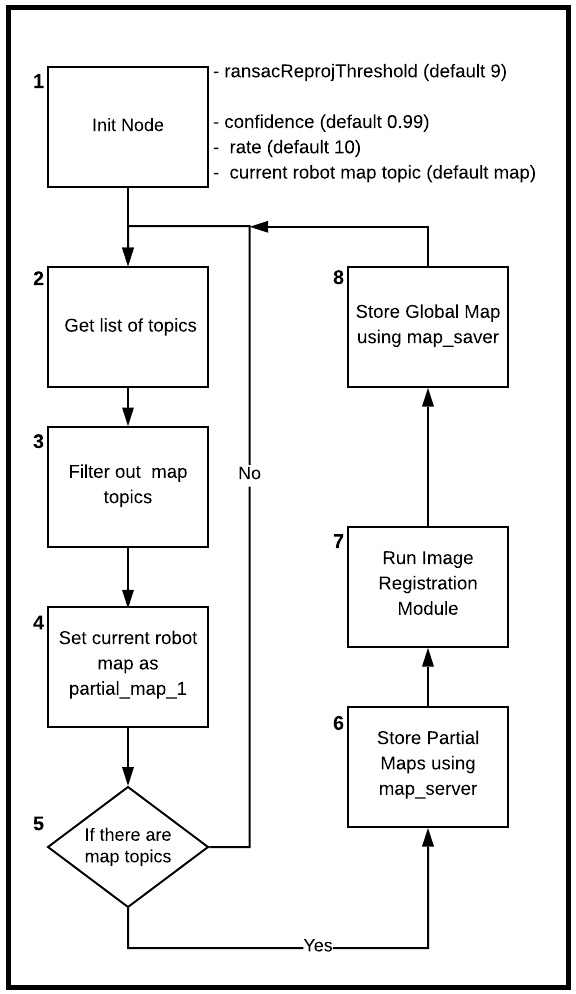
\includegraphics[width=0.6\textwidth]{UCT_MSc_Thesis/figs/implementation/ROSnodeImplementation.jpg}
    \caption{ROS node implementation.}
    \label{fig:ros-node-implementation}
\end{figure}
\


\section{Summary}

In this chapter, a multi-robot multi-session map merging approach is presented. In the next chapter, validation experiments run in simulation and real-world scenarios are discussed. The simulation tests were conducted using two and three partial maps at different resolutions, and so are the real-world experiments.

 % Implementation
% !TeX spellcheck = en_GB
%****************************************************
%	CHAPTER Experimental Validation
%****************************************************

%====================================================
\chapter{Experimental validation}
\label{ch:experimental}
%----------------------------------------------------

This chapter describes and discusses the experimental methods and results used to validate the solution proposed in Chapter \ref{ch:implementation}. 

%====================================================
\section{Introduction}
\label{sec:ch4.section1}
%----------------------------------------------------
The results were obtained using a distributed approach where each robot is tasked with both map generation and the full map merging process(alignment and merging) to obtain a global map relative to its local map.

Experimental tests were performed in both simulation and real-world scenarios to evaluate the proposed solution's performance. For the real-world scenarios data generated for the proposes of this thesis is used, alongside publicly available data collected in the Maria Stata Center at MIT. This data from MIT has also been used in \cite{8250173, 7849536, doi:10.1177/0278364915614638}. The data-sets generated and used can be found on \href{https://drive.google.com/drive/folders/1c\_2-T8FcrSmE0VDyHw20-jRLHKRuAvpE}{Google drive}. Given that the proposed solution in the previous chapter is aimed at multi-session, multi-robot and multi-resolution map merging, this requires several robots generating maps during multiple sessions at varying map resolution in indoor environments.

In all the experiments, ROS is used to both record and process the data. The data is recorded and saved as \(rosbag\) files, and these files are then used to generate the partial maps, at different resolutions.

%====================================================
\section{Hector mapping parameters}
%----------------------------------------------------

Hector mapping which is discussed in a previous chapter\ref{ch:ch2}, is used to generate the partial maps. The parameters will be kept as default except for the frame parameters(which are \textit{base\_frame}, \textit{map\_frame} and \textit{odom\_frame}), \textit{map\_resolution}  and \textit{map\_size}. The frame parameters are changed to match the robot frame. The \textit{map\_resolution} is varied to evaluate the solutions ability to deal with multiple resolutions. Finally, the\textit{map\_size} is varied to match the environment size. Unlike \textit{gmapping}, \textit{hector\_mapping} maps do not change size dynamically therefore a static value must be set.

%====================================================
\section{Performance measures}
%----------------------------------------------------

The following performance measures are presented alongside the resultant global map of the map merging operation. 

\textbf{Resolution and calculated resolution}

Assume that we have $map_1$ and $map_2$, where $map_2$
is transformed into $map_1$'s frame of reference. Then the calculated new resolution of $map_2$ should be within 
%....................................................
\begin{align*}
%----------------------------------------------------
    1-confidence &= 1 - 0.99 \\
    & = 0.01  
%----------------------------------------------------
\end{align*}
%....................................................

of the resolution of $map_1$. This performance measure is there to confirm that the error checking of the algorithm performs adequately.

\textbf{Angle of rotation}

The angle of rotation is computed from the affine matrix, shown in Equation \ref{eq:rotat_scale}. The angle is presented to show the angle which maps were rotated through to match the reference map.

\textbf{Good matches and Match ratio}

The good matches represent the number of features matched between to maps. These matches are presented with their corresponding match ratio. The match ratio introduced here is the same match ratio introduced in Section\ref{sub:sec:method}. The match ratio is determined by:

%....................................................
\begin{equation}
%----------------------------------------------------
    \frac{matches}{\min(num\_features\_map_1, num\_features\_map_2)}
%----------------------------------------------------
    \label{eg:match_ratio}
%----------------------------------------------------
\end{equation}
%....................................................

, where $num\_features$ is the number of features, and $matches$ is the number of matches found between $map_1$ and $map_2$ features, using the earlier discussed Brute-Force matcher. The higher the match ratio, the more matches were found between the two maps. 


\textbf{Percentage overlap}

Assume we are merging two images, for the images to be merged an overlapping area is required to find matching features. The percentage of overlap is described by:
%....................................................
\begin{equation}
%----------------------------------------------------
    P_{overlap} = \frac{A_{overlap}}{A_{1} + A_{2} - A_{overlap}} \times 100
%----------------------------------------------------
\end{equation} 
%....................................................
Here, $A_1$ is the occupied and unoccupied area of $map_1$, $A_2$ is the occupied and unoccupied area of $map_2$ and $A_{overlap}$ is the occupied and unoccupied of the overlapping area.
The following sections focus on simulation results, followed by real-world results produced in this work and from the MIT Stata Center dataset\cite{doi:10.1177/0278364913509035}. In each experiment, the global map is produced relative to partial map\_1. Therefore the global map takes on the resolution of partial map\_1. 


%====================================================
\section{Simulation experiments}
\label{subsec:ch4.section1.subsec1}
%----------------------------------------------------
This section presents experiments done with a simulated using a ROS and Gazebo. The experiments were performed to evaluate the performance of map merging algorithm on 2 and 3 robots. The simulation environment set up is described in Section\ref{subsec:sim:environment_set_up}. The map merging algorithm results are presented in Section\ref{sec:sim_results}.

%====================================================
\subsection{Environment setup}
\label{subsec:sim:environment_set_up}
%----------------------------------------------------

Gazebo is an open-source simulation environment, which offers an accurate and efficient simulation of indoor and outdoor robots, a robust physics (such as illumination, gravity and inertia) engine, high-quality graphics and a graphical interfaces. Gazebo also works alongside ROS, allowing for simulated development and testing. To achieve ROS integration with stand-alone Gazebo, a set of ROS packages named \textit{gazebo\_ros\_pkgs} provides wrappers around the stand-alone Gazebo. The wrappers provide the necessary interfaces to simulate robots in Gazebo using ROS messages, services and dynamic reconfigure \cite{Quigley2009}. The use of Gazebo enables the testing of scenarios without the need for a fully functional robot team, which are usually expensive. It also eliminates the limitation of battery life, which can be ignored in a simulation environment.



The main components of Gazebo are:
%....................................................
\begin{itemize}
%----------------------------------------------------
\item \textbf{World file} - This file contains all the elements in the simulation world, such as robots, lights, sensors, and static objects.
%----------------------------------------------------
\item \textbf{Models} - The purpose of these files is to facilitate model reuse and simplify world files.
%----------------------------------------------------
\item \textbf{gzserver} - This server reads the world file and models to generate the simulation world.
%----------------------------------------------------
\item \textbf{gzclient} -The client connects to a running \(gzserver\) and visualises the simulation environment. This client also allows the user to modify the simulation environment, shown in Figure \ref{fig:gazebo-environment}.
%----------------------------------------------------
\end{itemize}
%....................................................

%....................................................
\begin{figure}[H]
%----------------------------------------------------
    \centering
%----------------------------------------------------
    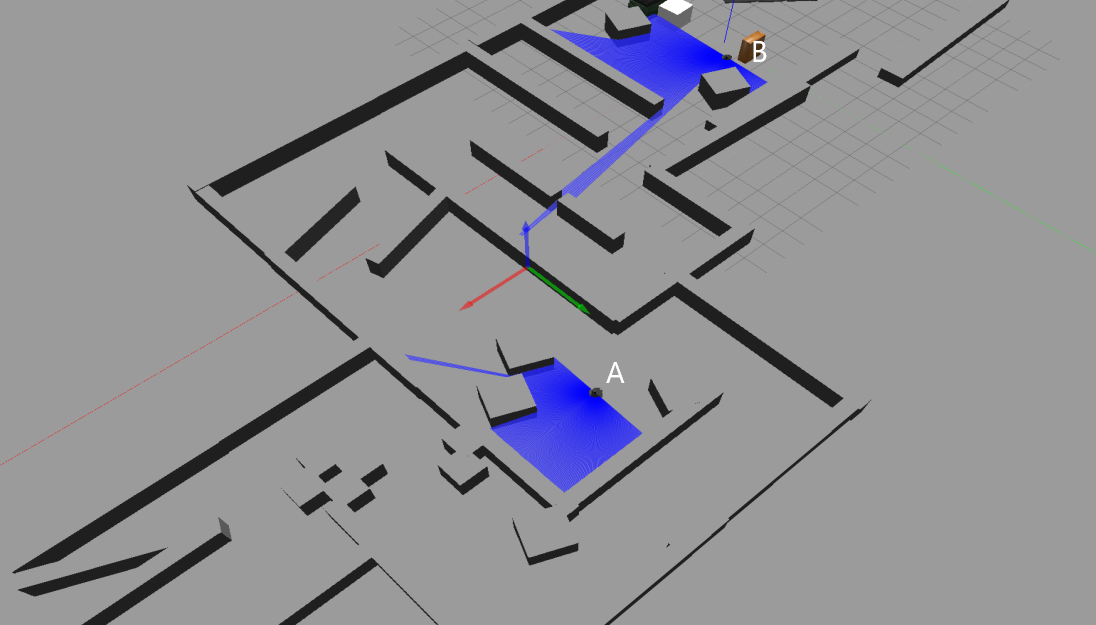
\includegraphics[width=1\textwidth]{figs/gazebo_environment.png}
%----------------------------------------------------
    \caption{Gazebo \(gzclient\) generated from the \(gzserver\). The \(gzserver\) generated the simulation world using a world file and model files. This figure describes two robots (annotated by A and B) and lidar sensor (which are the blue rays are laser rays) in an environment.}
%----------------------------------------------------
    \label{fig:gazebo-environment}
\end{figure}
%....................................................



Figure \ref{fig:maze_arena}, is the layout of the simulation environment used in this experiment. The environment shows two robots simulated in Gazebo building partial maps of the environment, a transform tree diagram with the coordinate frames associated with each robot is presented in Figure \ref{fig:rosgraph-gazebo}, each frame having a prefix to inform ROS which robot it belongs to. The graph also shows the average rate of message exchange transforms and the existing frames of the robots. The simulated robots are Kobuki platforms (see Figure \ref{fig:kuboki-platform-gazebo}) equipped with Hokuyo laser range finders, these robots are selected to match the real-world robot platform used. The simulated Kokoki Platform is controlled using the \(turtlebot\_teleop\)\footnote{http://wiki.ros.org/turtlebot\_teleop} node, through the keyboard. The simulated environment is run on a Windows 10 laptop with the following specifications; Intel Core i5-8250U processor with 16 GB of RAM. The simulated environment is run on a virtual machine using VirtualBox, and the machine can be found on \footnote{googledrive}. The simulated environment is used to initially test the solution proposed in a controlled environment with known parameters. 

%....................................................
\begin{figure}[H]
%----------------------------------------------------
    \centering
%----------------------------------------------------
    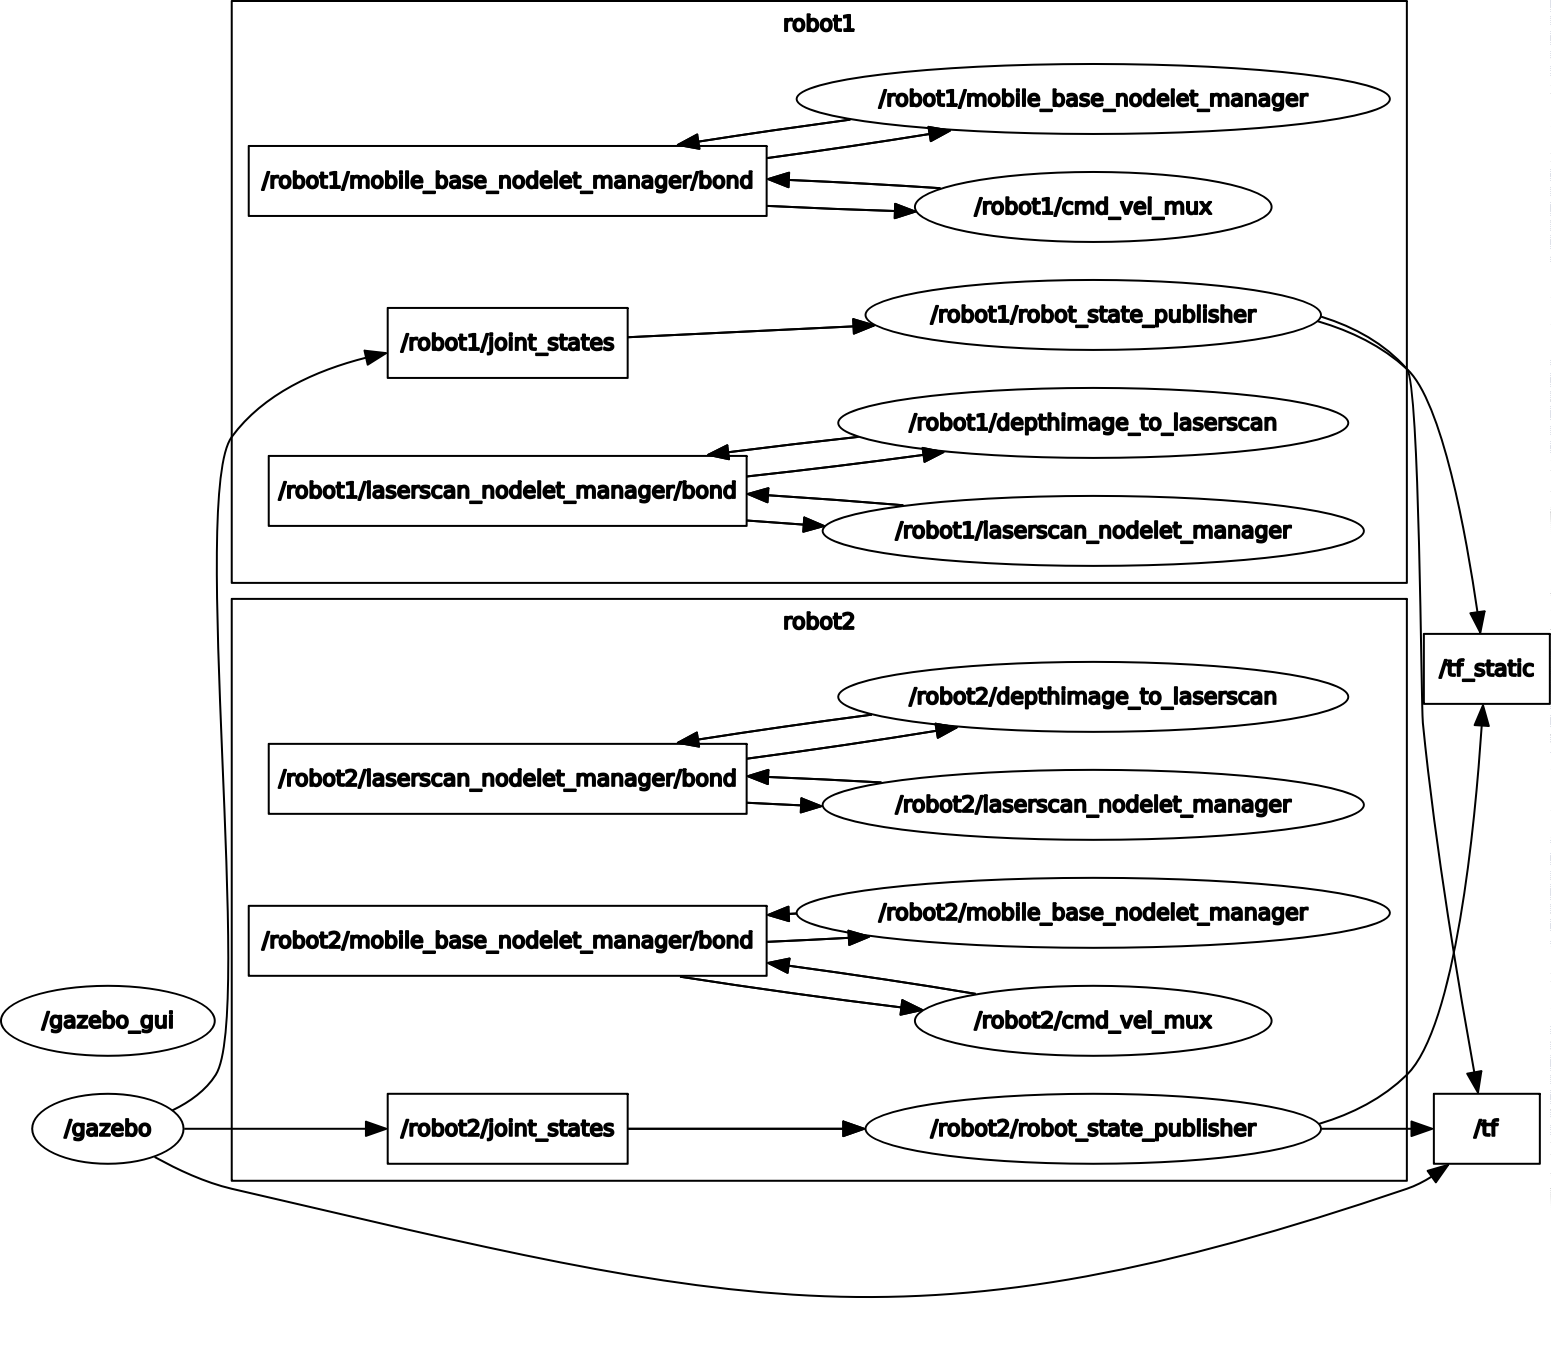
\includegraphics[width=0.9\textwidth]{figs/rosgraph.png}
%----------------------------------------------------
    \caption{ROS graph for simulation environment shown in Figure \ref{fig:gazebo-environment}.}
%----------------------------------------------------
    \label{fig:rosgraph-gazebo}
%----------------------------------------------------
\end{figure}
%....................................................


%....................................................
\begin{figure}[H]
    \centering
    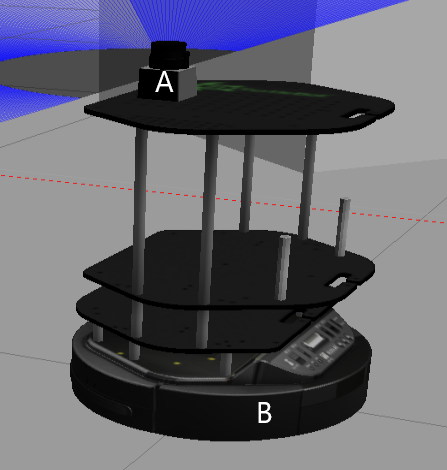
\includegraphics[width=0.5\textwidth]{figs/Kuboki_Platform_Gazebo.png}
    \caption{Kobuki Platform (annotated by (B)) in Gazebo environment. The Platform has a Hokuyo UTM-30LX (annotated by (A) also simulated. Note that the laser rays (blue lines) were limited to 180 degrees. This is all simulated using Gazebo.}
    \label{fig:kuboki-platform-gazebo}
\end{figure}
%....................................................

%....................................................
\begin{figure}[H]
    \centering
    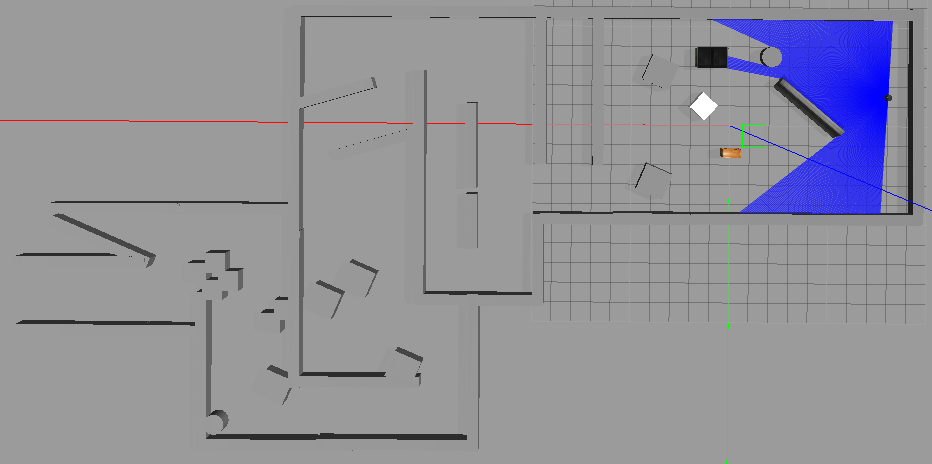
\includegraphics[width=1\textwidth]{figs/maze_area.png}
    \caption{Gazebo simulation environment, with obstacle around the map. There is a Kobuki Platform, with a Hokuyo UTM-30LX attached to it, these are also simulated. }
    \label{fig:maze_arena}
\end{figure}
%....................................................

%====================================================
\subsection{Results and discussion}
\label{sec:sim_results}
%----------------------------------------------------
In this section, simulation results using Gazebo and ROS are presented. 

%==================================================== 
\subsubsection{Experiment one} %----------------------------------------------------

Figures \ref{fig:sim11} and \ref{fig:sim12} represent each robot's partial local map before the merging operation. The local partial maps have a resolution of 0.1 m/cell. Figure \ref{fig:sim13} presents the global map with a resolution of 0.1 m/cell, after merging the partial maps. The global map shows that the partial maps were adequately aligned and merged. The new resolution of partial\_map\_2 is within 1\% of partial\_map\_1's resolution (shown in Table \ref{table:sim1}), therefore validating the success of the alignment operation.  

%....................................................
\begin{figure}[H]
%----------------------------------------------------
\begin{subfigure}{0.5\textwidth}
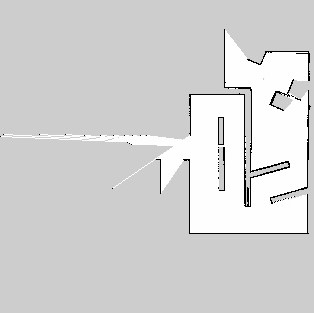
\includegraphics[width=0.9\linewidth, height=5cm]{figs/simulation_results/a/partial_map_1.jpg} 
\caption{Partial map\_1 with resolution of 0.1 m/cell}
\label{fig:sim11}
\end{subfigure}
%----------------------------------------------------
\begin{subfigure}{0.5\textwidth}
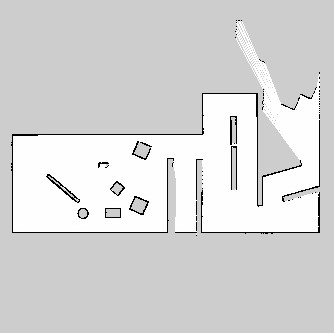
\includegraphics[width=0.9\linewidth, height=5cm]{figs/simulation_results/a/partial_map_2.jpg} 
\caption{Partial map\_2 with resolution of 0.1 m/cell}
\label{fig:sim12}
\end{subfigure}
%----------------------------------------------------
\begin{subfigure}{0.5\textwidth}
\centering
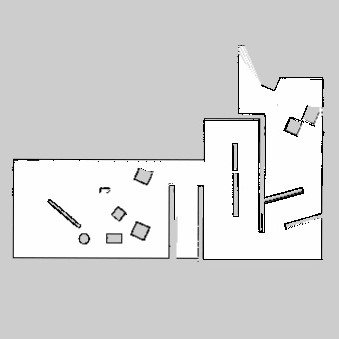
\includegraphics[width=0.9\linewidth, height=5cm]{figs/simulation_results/a/final_map.jpg} 
\caption{Global map with resolution of 0.1 m/cell}
\label{fig:sim13}
\end{subfigure}
%----------------------------------------------------
\caption{Partial maps and a global map are presented. The partial maps are generated from simulated data. Since the maps are aligned relative to map\_1, the resultant global map will have the same resolution as partial map\_1.}
\label{fig:sim1}
\end{figure}
%....................................................

Figure \ref{fig:sim1match1} presents the matched features in the partial maps' overlapping area. There are 30 matched features with a match ratio of 0.46, where the percentage of overlapping area is 35.36\% (see Table \ref{table:sim1}). The match ratio value is influenced by the fact that partial\_map\_2 has most of its features within the overlapping area.


%....................................................
\begin{figure}[H]
    \centering
    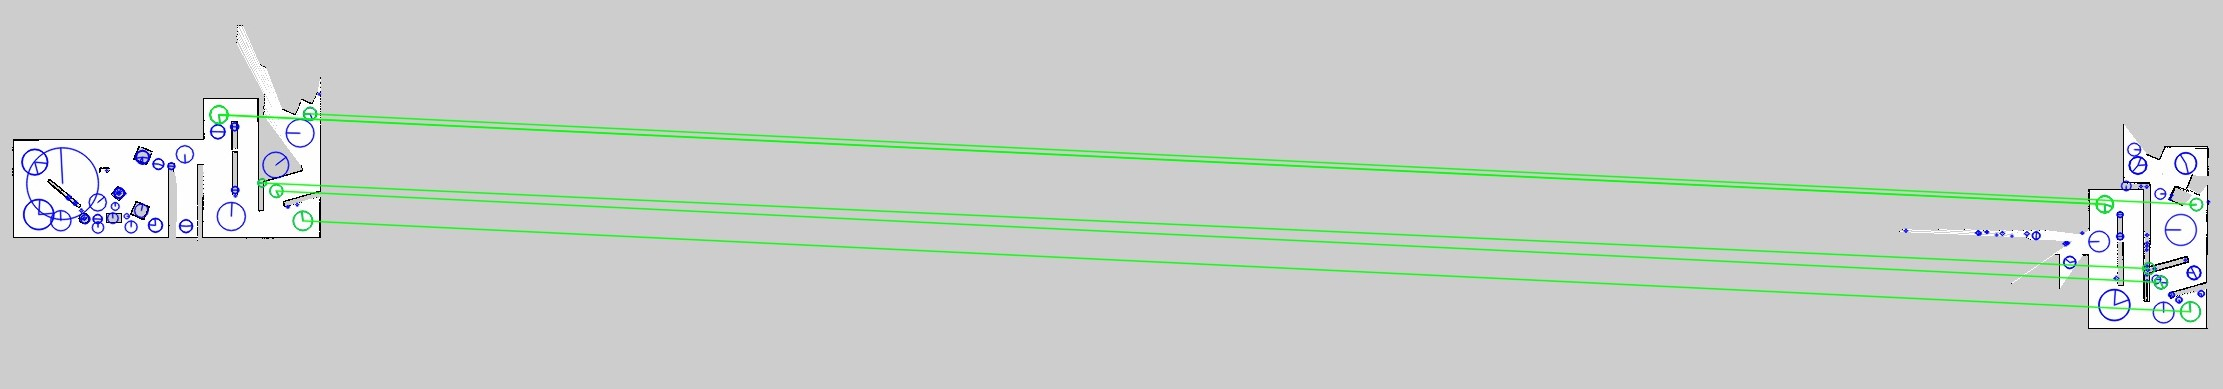
\includegraphics[width=1\textwidth]{figs/simulation_results/a/matchesPartialMap1Map2.jpg}
    \caption{The matched features between partial map\_1 and map\_2 are presented in this figure. The features highlighted in green, are the features that have been matched between the two maps.}
    \label{fig:sim1match1}
\end{figure} 
%....................................................

%....................................................
\begin{table}[H]
\centering
\caption{This table presents the results from the alignment and merging operation. Since the partial maps are merged relatively to map\_1, the results are relative to map\_1, which has a resolution of 0.1 m/cell.}

%----------------------------------------------------
\begin{tabular}{ | m{1.4cm} | m{2.2cm} | m{2.2cm} | m{2.4cm} | m{1.7cm} | m{1.4cm} | m{2.4cm} | } 
\hline
\textbf{Map} & \textbf{Resolution (m/cell)} & \textbf{New resolution (m/cell)} & \textbf{Angle of rotation (\degree)} & \textbf{Good matches} & \textbf{Match ratio} & \textbf{Percentage overlap}\\ 
\hline 
\hline
Partial map\_2  & 0.1  & 0.09956828 & -0.16716242 & 30 & 0.46 & 35.36 \\ 
\hline
\end{tabular}
%----------------------------------------------------
\label{table:sim1}
\end{table}
%....................................................

%==================================================== 
\subsubsection{Experiment two} 
%----------------------------------------------------

The next results still consider two robots with the same resolution partial\_maps, but the maps have a bigger overlapping area of 48.03\% (see Table \ref{table:sim2}). Figures \ref{fig:sim21} and \ref{fig:sim22} represent each robot's partial local map before the merging operation. The local partial maps have a resolution of 0.1 m/cell. Figure\ref{fig:sim13} presents the global map of 0.1 m/cell, after the merging of the partial maps. The global map shows that the partial maps were adequately aligned and merged. The new resolution of partial\_map\_2 is within 1\% of partial\_map\_1's resolution (shown in Table \ref{table:sim2}), therefore validating the success of the alignment operation.  

%....................................................
\begin{figure}[H]
%----------------------------------------------------
\begin{subfigure}{0.5\textwidth}
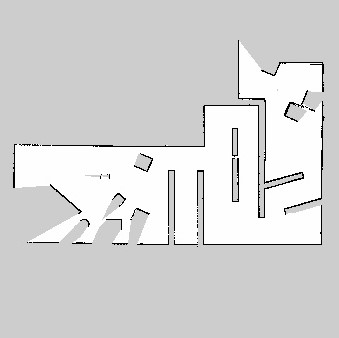
\includegraphics[width=0.9\linewidth, height=5cm]{figs/simulation_results/b/partial_map_1.jpg} 
\caption{Partial map\_1 resolution of 0.1 m/cell}
\label{fig:sim21}
\end{subfigure}
%----------------------------------------------------
\begin{subfigure}{0.5\textwidth}
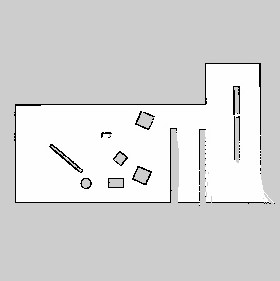
\includegraphics[width=0.9\linewidth, height=5cm]{figs/simulation_results/b/partial_map_2.jpg} 
\caption{Partial map\_2 resolution of 0.1 m/cell}
\label{fig:sim22}
\end{subfigure}
%----------------------------------------------------
\begin{subfigure}{0.5\textwidth}
\centering
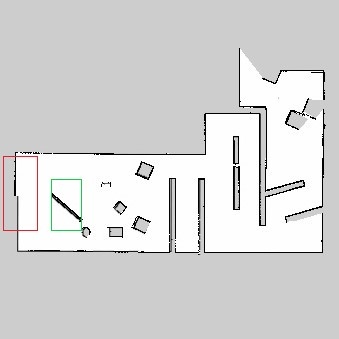
\includegraphics[width=0.9\linewidth, height=5cm]{figs/simulation_results/b/final_map_marked.jpg}
\caption{Global map of resolution of 0.1 m/cell}
\label{fig:sim23}
\end{subfigure}
%----------------------------------------------------
\caption{Partial maps and a global map are presented. The partial maps are generated from simulated data. Since the maps are aligned relative to map\_1, the resultant global map will have the same resolution as partial map\_1.}
\label{fig:sim2}
\end{figure}
%....................................................


Unlike results Figure \ref{fig:sim1}, Figure \ref{fig:sim2} a slight misalignment which is highlighted in red and green. Figure \ref{fig:sim2match1} shows that the features in the green and red area were not matched, therefore causing the misalignment. Despite the fact that the match ratio and percentage overlap of 0.59 and 48\%, are higher here (see Table \ref{table:sim2}) than in the previous ((see Table \ref{table:sim1}) results. This result suggests that it is important that the matches are evenly distributed throughout the overlapping region with a high match ratio. 

%....................................................
\begin{figure}[H]
    \centering
    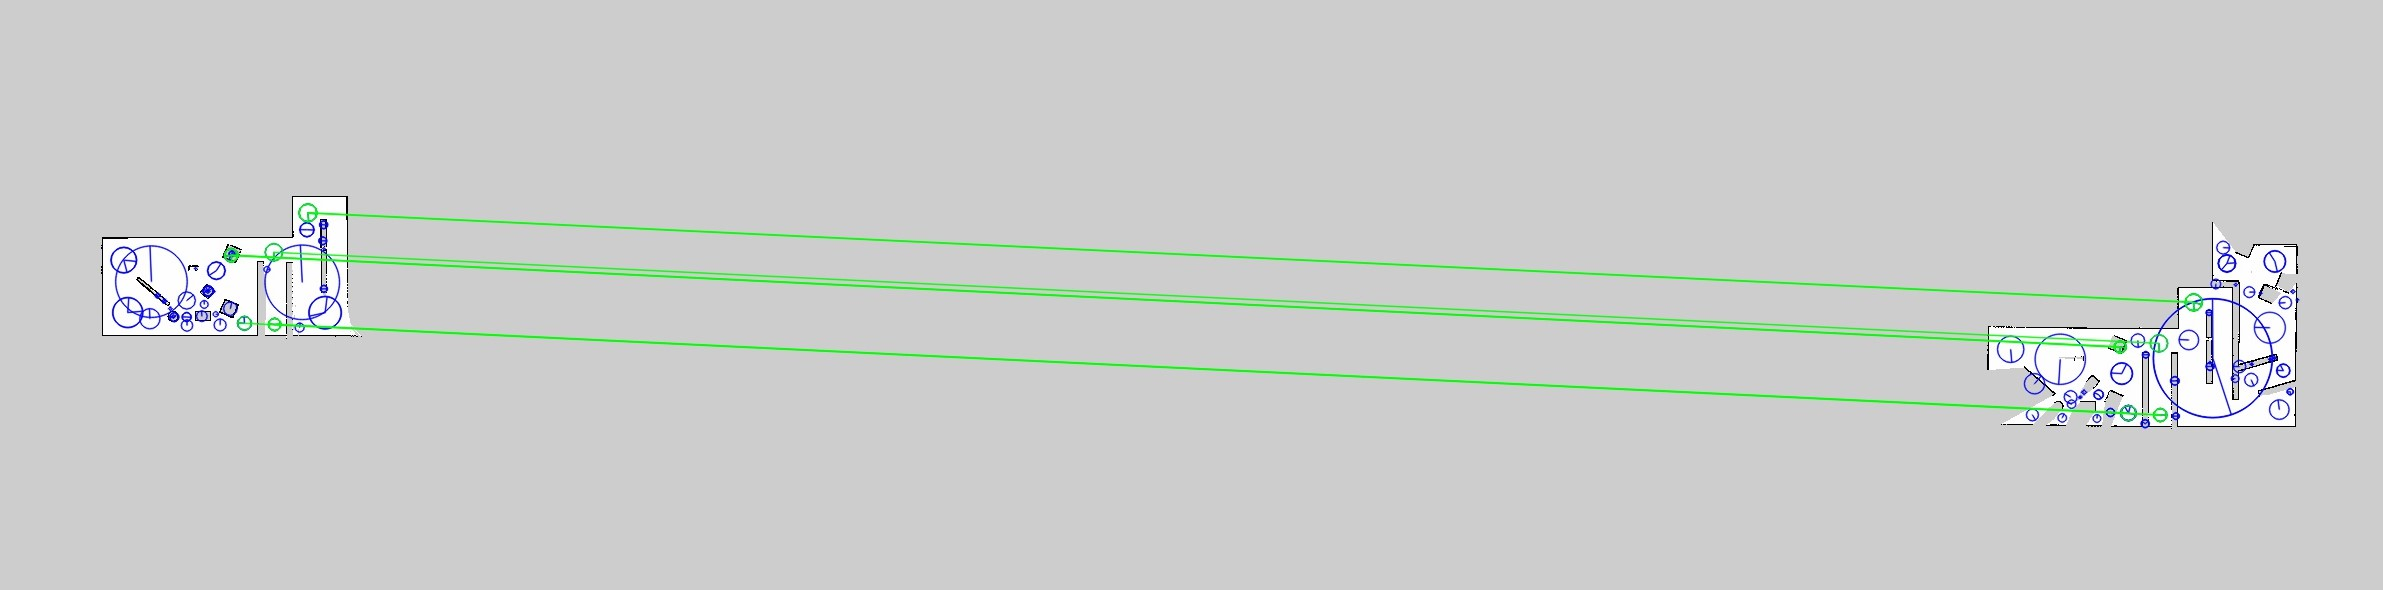
\includegraphics[width=1\textwidth]{figs/simulation_results/b/matchesPartialMap1Map2.jpg}
    \caption{The matched features between partial map\_1 and map\_2 are presented in this figure. The features highlighted in green, are the features that have been matched between the two maps.}
    \label{fig:sim2match1}
\end{figure} 
%....................................................



%....................................................
\begin{table}[H]
\centering
\caption{This table presents the results from the alignment and merging operation. Since the partial maps are merged relatively to map\_1 the results are relative to map\_1, which  has a resolution of 0.1 m/cell.}
\begin{tabular}{ | m{1.4cm} | m{2.2cm} | m{2.2cm} | m{2.4cm} | m{1.7cm} | m{1.4cm} | m{2.4cm} | }
\hline
\textbf{Map} & \textbf{Resolution (m/cell)} & \textbf{New resolution (m/cell)} & \textbf{Angle of rotation (\degree)} & \textbf{Good matches} & \textbf{Match ratio} & \textbf{Percentage overlap}\\ 
\hline
\hline
Partial map\_2  & 0.1  & 0.10111790 & -0.08469242 & 36 & 0.59 & 48.03\\ 
\hline
\end{tabular}
\label{table:sim2}
\end{table}
%....................................................

%==================================================== 
\subsubsection{Experiment three} %----------------------------------------------------

Figures \ref{fig:sim31}, \ref{fig:sim32} and \ref{fig:sim33} represent partial maps from three robots before the merging operation. The local partial maps have a resolution of 0.1 m/cell. The maps are to be transformed into partial\_map\_1's frame of reference. Figure \ref{fig:sim34} presents the global map of 0.1 m/cell, after merging the partial maps. The global map shows that the partial map\_2 and map\_3 were adequately aligned into map\_1 and merged. The new resolution of partial\_map\_2 and partial\_map\_3 are both within 1\% of partial\_map\_1's resolution (shown in Table \ref{table:sim3}) validating the success of the alignment operation.  

%....................................................
\begin{figure}[H]
\begin{subfigure}{0.5\textwidth}
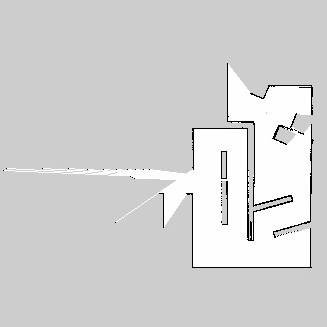
\includegraphics[width=0.9\linewidth, height=5cm]{figs/simulation_results/c/partial_map_1.jpg} 
\caption{Partial map\_1 with resolution of 0.1 m/cell}
\label{fig:sim31}
\end{subfigure}
\begin{subfigure}{0.5\textwidth}
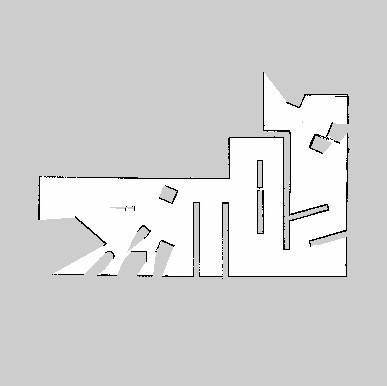
\includegraphics[width=0.9\linewidth, height=5cm]{figs/simulation_results/c/partial_map_2.jpg} 
\caption{Partial map\_2 with resolution of 0.1 m/cell}
\label{fig:sim32}
\end{subfigure}
\begin{subfigure}{0.5\textwidth}
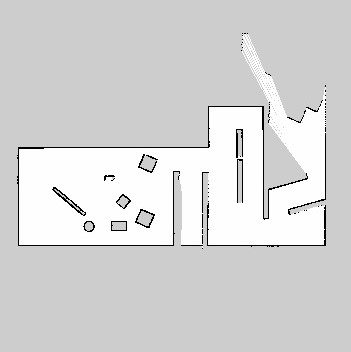
\includegraphics[width=0.9\linewidth, height=5cm]{figs/simulation_results/c/partial_map_3.jpg} 
\caption{Partial map\_2 with resolution of 0.1 m/cell}
\label{fig:sim33}
\end{subfigure}
\begin{subfigure}{0.5\textwidth}
\centering
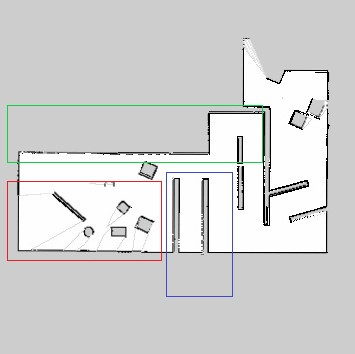
\includegraphics[width=0.9\linewidth, height=5cm]{figs/simulation_results/c/final_map_marked.jpg} 
\caption{Global map with resolution of 0.1 m/cell}
\label{fig:sim34}
\end{subfigure}
\caption{Three partial maps and a global map are presented. The partial maps are generated from simulated data. Since the maps are aligned relative to map\_1, the resultant global map will have the same resolution as partial map\_1.}
\label{fig:sim3}
\end{figure}
%....................................................


Given that the matches are mostly on the rightmost position (see figures \ref{fig:sim3match1} and  \ref{fig:sim3match2}) due to partial map\_1, results similar to Figure \ref{fig:sim2} are expected. The red regions in Figure \ref{fig:sim34} have unknown(grey) regions, likely because map\_2 and map\_3 are unaware of each other. However, the blue and green region in Figure \ref{fig:sim34} shows information from map\_2 and map\_3 being successfully included in the global\_map. 

Table \ref{table:sim3} shows match ratio results and percentage overlap, suggesting that a higher percentage produces a higher match ratio. This relationship will be evaluated in the next experiments too.

%....................................................
\begin{figure}[H]
    \centering
    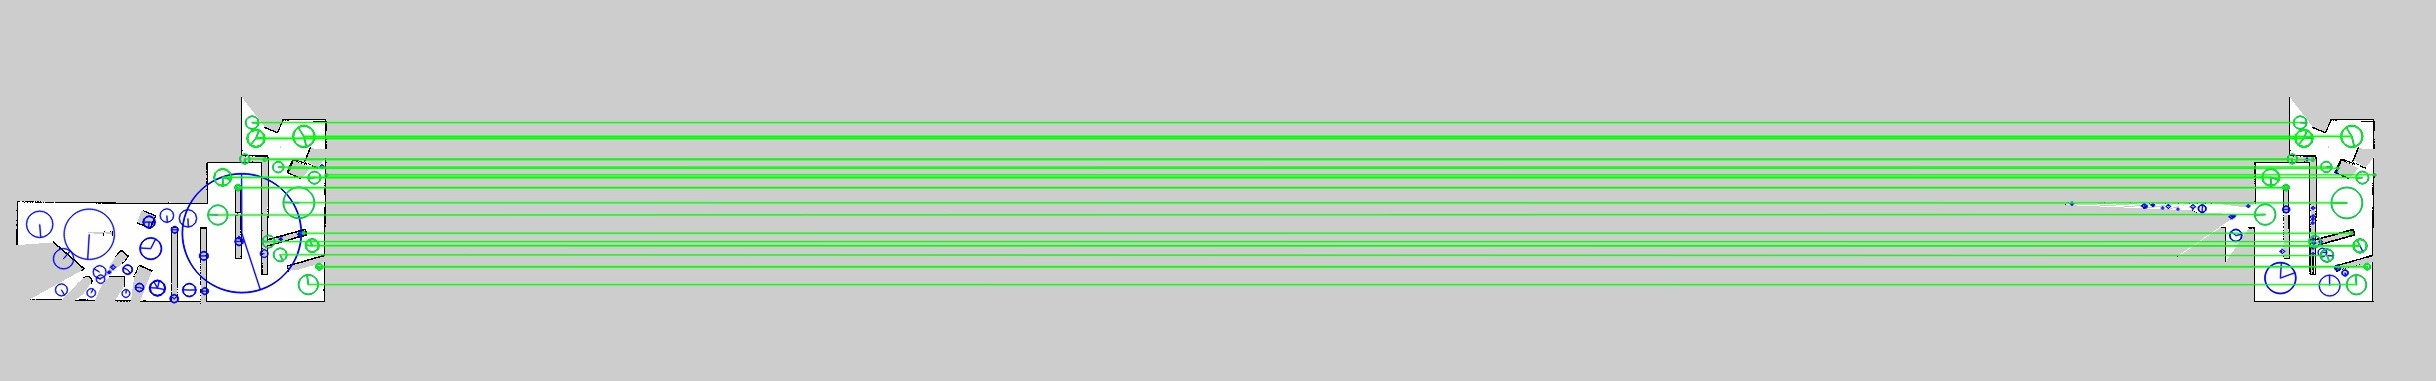
\includegraphics[width=1\textwidth]{figs/simulation_results/c/matchesPartialMap1Map2.jpg}
    \caption{The matched features between partial map\_1 and map\_2 are presented in this figure. The features highlighted in green, are the features that have been matched between the two maps.}
    \label{fig:sim3match1}
\end{figure} 
%....................................................

%....................................................
\begin{figure}[H]
    \centering
    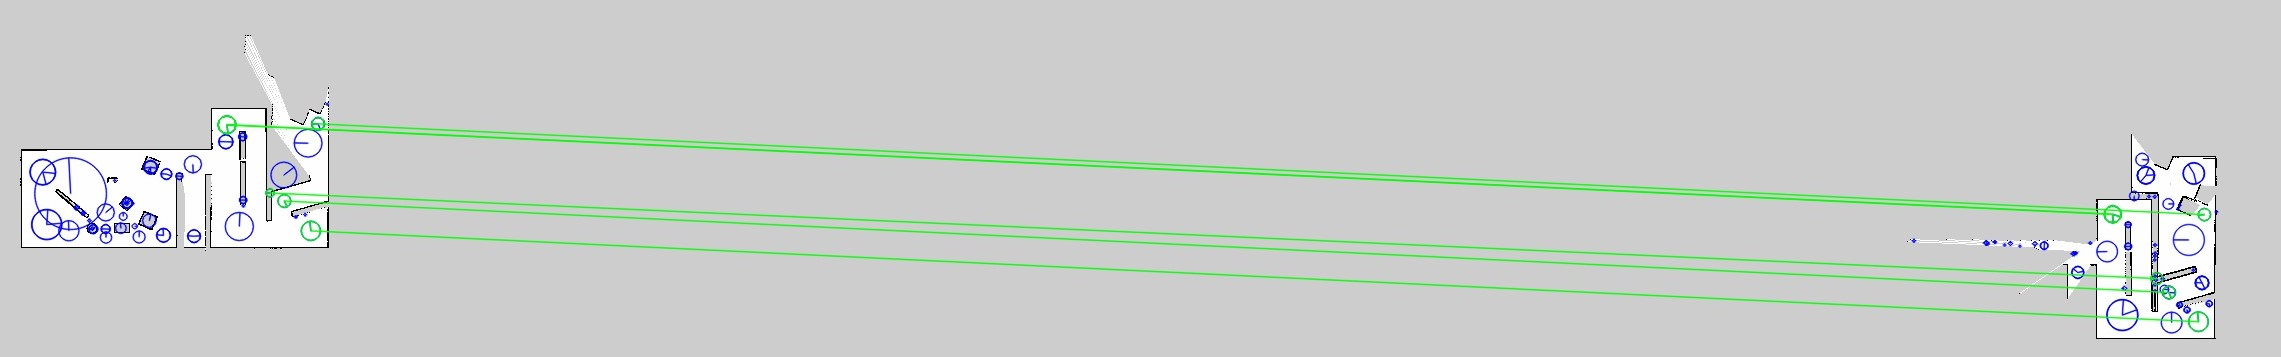
\includegraphics[width=1\textwidth]{figs/simulation_results/c/matchesPartialMap1Map3.jpg}
    \caption{The matched features between partial map\_1 and map\_3 are presented in this figure. The features highlighted in green, are the features that have been matched between the two maps.}
    \label{fig:sim3match2}
\end{figure} 
%....................................................

%....................................................
\begin{table}[H]
\centering
\caption{This table presents the results from the alignment and merging operation. Since the partial maps are merged relatively to map\_1 the results are relative to map\_1, which  has a resolution of 0.1 m/cell.}

\begin{tabular}{ | m{1.4cm} | m{2.2cm} | m{2.2cm} | m{2.4cm} | m{1.7cm} | m{1.4cm} | m{2.4cm} | } 
\hline
\textbf{Map} & \textbf{Resolution (m/cell)} & \textbf{New resolution (m/cell)} & \textbf{Angle of rotation (\degree)} & \textbf{Good matches} & \textbf{Match ratio} & \textbf{Percentage Overlap}\\ 
\hline
\hline
Partial map\_2  & 0.1  & 0.09985444 & -0.13717321 & 40 & 0.56 & 50.83502376\\ 
\hline
Partial map\_3  & 0.1  & 0.09956828 & -0.16716242 & 30 & 0.46 & 35.36\\ 
\hline
\end{tabular}
\label{table:sim3}
\end{table}
%....................................................


%==================================================== 
\subsubsection{Experiment four} 
%----------------------------------------------------

Figures \ref{fig:sim41} and \ref{fig:sim42} represents the partial maps of two robots at different resolutions (0.2 m/cell and 0.1 m/cell) before the alignment and merging operation. Partial\_map\_1 in Figure \ref{fig:sim41}, presents a mapping error highlighted in yellow, compared with original arena in Figure \ref{fig:maze_arena}. The mapping error has caused the map in the yellow region to rotate slightly. Despite the error a global map was successfully produced (see Figure \ref{fig:sim43}). These merging defects can be seen mostly in the red and green regions of the global\_map(Figure \ref{fig:sim43}); however the defects the information of partial\_map 2 have successfully been included in the map. The new resolution of partial\_map\_2 is with in 1\% of partial\_map\_1, which further validates the success of the merge (see Table \ref{table:sim4}).


%....................................................
\begin{figure}[H]
\begin{subfigure}{0.5\textwidth}
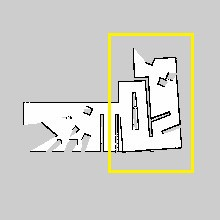
\includegraphics[width=0.9\linewidth, height=5cm]{figs/simulation_results/c_diff_resolution/partial_map_1_marked.jpg} 
\caption{Partial map\_1 with resolution of 0.2 m/cell}
\label{fig:sim41}
\end{subfigure}
\begin{subfigure}{0.5\textwidth}
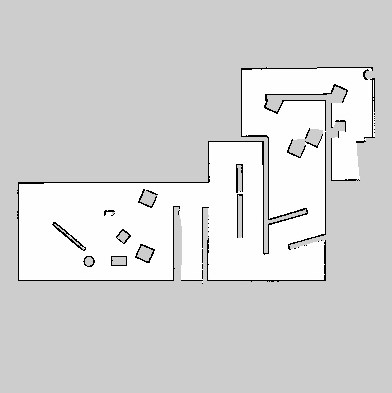
\includegraphics[width=0.9\linewidth, height=5cm]{figs/simulation_results/c_diff_resolution/partial_map_2.jpg} 
\caption{Partial map\_2 with resolution of 0.1 m/cell}
\label{fig:sim42}
\end{subfigure}
\begin{subfigure}{0.5\textwidth}
\centering
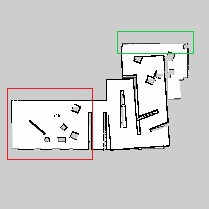
\includegraphics[width=0.9\linewidth, height=5cm]{figs/simulation_results/c_diff_resolution/final_map_marked.jpg} 
\caption{Global map with resolution of 0.2 m/cell}
\label{fig:sim43} 
\end{subfigure}
\caption{Two partial maps and a global map are presented. The partial maps are generated from simulated data, and they are of varying resolution. Since the maps are aligned relative to map\_1, the resultant global map will have the same resolution as partial map\_1.}
\label{fig:sim4}
\end{figure}
%....................................................


Figure \ref{fig:sim4match1} represents the matches between partial\_maps 1 and 2, with a match ratio of 0.66 and percentage overlap of 52.93\% (see Table \ref{table:sim4}). Again there is evidence of a directly proportional relationship between percentage overlap and match ratio compared to the previous experiment.


%....................................................
\begin{figure}[H]
    \centering
    \includegraphics[width=1\textwidth]{figs/simulation_results/c_diff_resolution/matchesPartialMap1Map2.jpg}
     \caption{The matched features between partial map\_1 and map\_2 are presented in this figure. The features highlighted in green, are the features that have been matched between the two maps.}
    \label{fig:sim4match1}
\end{figure} 
%....................................................

%....................................................
\begin{table}[H]
\centering
\caption{This table presents the results from the alignment and merging operation. Since the partial maps are merged relatively to map\_1 the results are relative to map\_1, which  has a resolution of 0.2 m/cell.}
\begin{tabular}{ | m{1.4cm} | m{2.2cm} | m{2.2cm} | m{2.4cm} | m{1.7cm} | m{1.4cm} | m{2.4cm} | }
\hline
\textbf{Map} & \textbf{Resolution (m/cell)} & \textbf{New resolution (m/cell)} & \textbf{Angle of rotation (\degree)} & \textbf{Good matches} & \textbf{Match ratio} & \textbf{Percentage overlap}\\ 
\hline
\hline
Partial map\_2  & 0.1  & 0.20177466 & 0.03968788 & 35 & 0.66 & 52.93\\ 
\hline
\end{tabular}
\label{table:sim4}
\end{table}
%....................................................

%==================================================== 
\subsubsection{Experiment five} %----------------------------------------------------

The final simulation experiment presents three partial maps aligned and merged to form a global map (see Figure \ref{fig:sim5}). Partial map\_2 and map\_3 have a resolution of 0.1 m/cell, which is different from map\_1's resolution of 0.2 m/cell. The global map in Figure \ref{fig:sim54}, is a result of the alignment and merging of maps 2 and 3 into map\_1's reference frame. Similarly to Figure \ref{fig:sim41}, Figure \ref{fig:sim51} has a mapping error, which has been incorporated into the global map. However, the errors both map\_2 and map\_3's new resolutions are within 1\% of map\_1's resolutions. 


%....................................................
\begin{figure}[H]
\begin{subfigure}{0.5\textwidth}
\includegraphics[width=0.9\linewidth, height=5cm]{figs/simulation_results/d_diff_resolution/partial_map_1.jpg} 
\caption{Partial map\_1 with resolution of 0.2 m/cell}
\label{fig:sim51}
\end{subfigure}
\begin{subfigure}{0.5\textwidth}
\includegraphics[width=0.9\linewidth, height=5cm]{figs/simulation_results/d_diff_resolution/partial_map_2.jpg} 
\caption{Partial map\_2 with resolution of 0.1 m/cell}
\label{fig:sim52}
\end{subfigure}
\begin{subfigure}{0.5\textwidth}
\includegraphics[width=0.9\linewidth, height=5cm]{figs/simulation_results/d_diff_resolution/partial_map_3.jpg} 
\caption{Partial map\_3 with resolution of 0.1 m/cell}
\label{fig:sim53}
\end{subfigure}
\begin{subfigure}{0.5\textwidth}
\centering
\includegraphics[width=0.9\linewidth, height=5cm]{figs/simulation_results/d_diff_resolution/final_map_marked.jpg} 
\caption{Global map with resolution of 0.2 m/cell}
\label{fig:sim54}
\end{subfigure}
\caption{Three partial maps and a global map are presented. The partial maps are generated from simulated data, and they are of varying resolutions. Since the maps are aligned relative to map\_1, the resultant global map will have the same resolution as partial map\_1.}
\label{fig:sim5}
\end{figure}
%....................................................

Figure \ref{fig:sim5match1} show feature matches between map\_1 and map\_2, with match ratio and percentage overlap of 0.68 and 54.43 respectively (see Table \ref{table:sim5}). Figure \ref{fig:sim5match1} shows feature matches between map\_1 and map\_3, with match ratio and percentage overlap of 0.52 and 27.62 respectively (see Table \ref{table:sim5}). This result again confirms the proportional relationship between the match ratio and percentage overlap.


%....................................................
\begin{figure}[H]
    \centering
    \includegraphics[width=1\textwidth]{figs/simulation_results/d_diff_resolution/matchesPartialMap1Map2.jpg}
    \caption{The matched features between partial map\_1 and map\_2 are presented in this figure. The features highlighted in green, are the features that have been matched between the two maps.}
    \label{fig:sim5match1}
\end{figure} 
%....................................................

%....................................................
\begin{figure}[H]
    \centering
    \includegraphics[width=1\textwidth]{figs/simulation_results/d_diff_resolution/matchesPartialMap1Map3.jpg}
    \caption{The matched features between partial map\_1 and map\_3 are presented in this figure. The features highlighted in green, are the features that have been matched between the two maps.}
    \label{fig:sim5match2}
\end{figure} 
%....................................................

%....................................................
\begin{table}[H]
\centering
\caption{This table presents the results from the alignment and merging operation. Since the partial maps are merged relatively to map\_1 the results are relative to map\_1, which  has a resolution of 0.2 m/cell.}
\begin{tabular}{ | m{1.4cm} | m{2.2cm} | m{2.2cm} | m{2.4cm} | m{1.7cm} | m{1.4cm} | m{2.4cm} | }
\hline
\textbf{Map} & \textbf{Resolution (m/cell)} & \textbf{New resolution (m/cell)} & \textbf{Angle of rotation (\degree)} & \textbf{Good matches} & \textbf{Match ratio} & \textbf{Percentage overlap}\\ 
\hline
\hline
Partial map\_2  & 0.1  & 0.1980208 & -17.8182736 & 36 & 0.68 & 54.43\\ 
\hline
Partial map\_3  & 0.1  & 0.2019860 & -2.91611928 & 24 & 0.52 & 27.62\\ 
\hline
\end{tabular}
\label{table:sim5}
\end{table}
%....................................................

\subsubsection{Summary}
The results in this section show that up-to three partial maps with different translations, orientations and resolutions can be aligned and merged successfully to form a global map. The results also show that mapping errors are propagated into the global map. The map merging operation can be limited by the matched feature spread. If matches are concentrated in one area, the merging operation will struggle to match other overlapping areas. We have also observed that the match ratio is directly proportional to the percentage overlap.

Further experiments can now be carried out to test the solution's real-world performance, using this section's results. The next section discusses the experiments carried out in the real world.



%====================================================

\section{Real-world experiments}
\label{subsec:ch4.section1.subsec2}
%----------------------------------------------------

The promising results from the simulation experiments naturally suggested transferring the experiments into the real-world. This section presents a real-world experiment setup and results.

%====================================================
\subsection{Environment setup}
%----------------------------------------------------

The experiments were conducted in the Leslie Social building at the University of Cape Town\footnote{http://www.uct.ac.za/main/contacts/building-list}. This building is a structured indoor environment with minimal natural lighting. Figure \ref{fig:uct_floor} is a floor plan of the fifth floor in the building, and the yellow highlight shows the path travelled by the robot. Using ROS's capability, the robot data is recorded using \(rosbag\)\footnote{http://wiki.ros.org/rosbag}, and later partial maps are generated at a varying resolution for merging.

\begin{figure}[H]
    \centering
    \includegraphics[width=1\textwidth]{figs/real_world_results/original_floor.png}
    \caption{Leslie Social 5th Floor at the University of Cape Town, the yellow shows where the robot moved during the experiment. The partial maps are produced in this area. }
    \label{fig:uct_floor}
\end{figure}


%====================================================
\subsubsection{Kuboki Platform}
%----------------------------------------------------

The chassis shown in Figure \ref{fig:kuboki-platform} is the iClebo Kobuki used in simulation and real-world testing. This platform is a low-cost mobile robot designed for education and research on the state of art robotics. The Kobuki provides power supplies for an external computer and any additional sensors.

%....................................................
\begin{figure}[H]
    \centering
    \includegraphics[width=0.9\textwidth]{figs/Kuboki_Platform.png}
    \caption[Kobuki platform]{Kobuki platform without attachments. Taken from \footnote{http://kobuki.yujinrobot.com/about2/}.}
    \label{fig:kuboki-platform} 
\end{figure}
%....................................................

The platform in Figure \ref{fig:turtle_bot_experiments}, is set up with a Hokuyo UTM-30LX and Raspberry Pi 3B with ROS installed. The Kobuki platform can travel at a maximum of 70 cm/s translational velocity, and a maximum rotational velocity of 180 \degree/s, however above 110 \degree/s performance will degrade. The platform can take a maximum payload of 5 kg. The platform has safety measures to ensure safe usage, and these include a cliff detector (to avoid driving off cliffs of a depth greater than 5cm) and a climbing threshold (to avoid climbing elevations above 12 mm). The expected operating time is 3/7hours (small/large battery), and the expected charging time is 1.5/2.6 hours (small/large battery). 

The Kobuki platform can be controlled using the Robot Operating System (ROS), a repository is provided on \footnote{https://github.com/yujinrobot/kobuki}. This repository also offers simulation models that can be used to simulate the platform in Gazebo or \textit{stage\_ros}.


 \begin{figure}[H]
    \centering
    \includegraphics[width=1\textwidth]{figs/real_world_results/turtle_bot.jpg}
    \caption{This figure shows the Kobuki Platform (C) used in the experiments. The platform is equipped with a  Hokuyo UTM-30LX (A) and a Raspberry Pi 3B (B) with ROS installed.}
    \label{fig:turtle_bot_experiments}
\end{figure}


%The chassis is equipped with the following:
%\begin{itemize}
%\item \textbf{Power Connectors}: 19V/2A, 12V/5A, 12v/1.5A and 5V/1A
%\item \textbf{Status Indicator LED}: Green - On, Orange- On but battery low, Green blinking - Battery charging %and if off the platform is off
%\item \textbf{Two Programmable LEDs}
%\item \textbf{USB Port}: For firmware update and platform communication
%\item \textbf{Three Touch Buttons}: These buttons can be used to as inputs
%\item \textbf{Firmware switch}: Enable/disables the firmware update mode
%\item \textbf{Battery}: Lithium-Ion, 14.8V, 2200 mAh (4S1P - small), 4400 mAh (4S2P - large)
%\item \textbf{Motor Overload Detection}: disables power on detecting high current (>3A)
%\item \textbf{Odometry}: 52 ticks/enc rev, 2578.33 ticks/wheel rev, 11.7 ticks/mm
%\item \textbf{Gyro}: factory calibrated, 1 axis (110 deg/s)
%\item \textbf{Bumper Sensors}: left, center, right
%\item \textbf{Cliff Sensors}: left, center, right
%\item \textbf{Wheel Drop Sensor}: left, right
%\item \textbf{Expansion Pins}: 3.3V/1A, 5V/1A, 4 x analogue in, 4 x digital in, 4 x digital out
%\item \textbf{Audio} : several programmable beep sequences
%\item \textbf{Sensor Data Rate}: 50Hz
%\end{itemize}

%====================================================
\subsubsection{Hokuyo UTM-30LX}
\label{sec:hokuyo}
%----------------------------------------------------

Attached to the Kobuki platform is a Hokuyo UTM-30LX (see Figure \ref{fig:hokuyo}), this is a dedicated laser range finder (LIDAR) used in many robotic applications. The sensor requires a 12 volts direct current power supply that can operate between 0.7 amperes and 1 amperes. This sensor uses a semiconductor laser diode with a wavelength (\(\lambda\)) of 905 nanometers. The Field of View (FOV) of the sensor is 270\(\degree\); hence the sensor will typically be mounted on top of the robot to maximise unobstructed FOV. The sensor has an accuracy of 30 millimetres at a range of 0.1 metres to 10 metres, and an accuracy of 50 millimetres at a range of 10 metres to 30 metres. This accuracy can be less reliable if the sensor receives intense light, such as sunlight directly in the outdoor environment. The sensor has an angular resolution of 0.25\(\degree\); this is the minimum angle between different objects in a scan. The sensor is equipped with a USB2.0 connector for communication with other devices.

\begin{figure}[H]
    \centering
    \includegraphics[width=0.3\textwidth]{figs/Hokuyo.png}
    \caption[Hokuyo UTM-30LX LIDAR]{Hokuyo UTM-30LX. Taken from \footnote{https://www.hokuyo-usa.com/products/scanning-laser-rangefinders/utm-30lx}}
    \label{fig:hokuyo}
\end{figure} 

%====================================================
\subsubsection{System integration}
%----------------------------------------------------

The Kobuki Platform is ROS compatible, which is installed on a Raspberry Pi 3B. ROS package turtlebot\_create\footnote{https://github.com/turtlebot/turtlebot\_create} is also installed to connect to the Kuboki platform, and commands are sent through a USB data connection to the platform. To control the motion of the platform and a Logitech F710 wireless gamepad (Figure \ref{fig:logitech_controller} alongside the ROS package \(turtlebot\_teleop\)\footnote{http://wiki.ros.org/turtlebot\_teleop} are used.
 

\begin{figure}[H]
    \centering
    \includegraphics[width=0.3\textwidth]{figs/real_world_results/logitech_controller.jpg}
    \caption{The Logitech Wireless Gamepad F710 uses a powerful and reliable cable-free 2.4 GHz connection while dual-motor vibration and is used to control the Kobuki Platform.}
    \label{fig:logitech_controller}
\end{figure}


%====================================================
\subsection{Results and discussion}
%----------------------------------------------------

In this section, results from real-world data are presented.

%==================================================== 
\subsubsection{Experiment one} %----------------------------------------------------

Figures \ref{fig:real11} and \ref{fig:real12} represents local partial maps from two robots. The local partial maps both have a resolution of 0.05 m/cell. Figure \ref{fig:real13} presents the global map with a resolution of 0.05 m/cell after the alignment and merging of the two partial maps. 

%....................................................
\begin{figure}[H]
\begin{subfigure}{0.5\textwidth}
\includegraphics[width=0.9\linewidth, height=5cm]{figs/real_world_results/b/partial_map_1.jpg} 
\caption{Partial map\_1 with resolution of 0.05 m/cell}
\label{fig:real11}
\end{subfigure}
\begin{subfigure}{0.5\textwidth}
\includegraphics[width=0.9\linewidth, height=5cm]{figs/real_world_results/b/partial_map_2.jpg} 
\caption{Partial map\_2 with resolution of 0.05 m/cell}
\label{fig:real12}
\end{subfigure}
\begin{subfigure}{0.5\textwidth}
\centering
\includegraphics[width=0.9\linewidth, height=5cm]{figs/real_world_results/b/final_map.jpg} 
\caption{Global map with a resolution of 0.05 m/cell}
\label{fig:real13}
\end{subfigure}
\caption{Two partial maps and a global map are presented. The partial maps are generated from real-world data. Since the maps are aligned relative to map\_1, the resultant global map will have the same resolution as partial map\_1.}
\label{fig:real1}
\end{figure}
%....................................................

The new resolution of partial\_map\_2 is within 1\% of partial\_map\_1's resolution (shown in Table \ref{table:real1}), therefore validating the success of the alignment operation. Figure \ref{fig:real1matches1} presents the matched features between the two partial maps, within the 29.78\% overlap region. There are 254 matched features with a match ratio of 0.50. There are significantly more features matched here than in the simulation environment. This result is due to the differing sizes of the maps. The real-world environment is larger than the simulation environment. 

%....................................................
\begin{figure}[H]
    \centering
    \includegraphics[width=1\textwidth]{figs/real_world_results/b/matchesPartialMap1Map2.jpg}
    \caption{The matched features between partial map\_1 and map\_2 are presented in this figure. The features highlighted in green, are the features that have been matched between the two maps}
    \label{fig:real1matches1}
\end{figure} 
%....................................................

%....................................................
\begin{table}[H]
\centering
\caption{This table presents the results from the alignment and merging operation. Since the partial maps are merged relatively to map\_1 the results are relative to map\_1, which  has a resolution of 0.05 m/cell.}
\begin{tabular}{ | m{1.4cm} | m{2.2cm} | m{2.2cm} | m{2.4cm} | m{1.7cm} | m{1.4cm} | m{2.4cm} | }
\hline
\textbf{Map} & \textbf{Resolution (m/cell)} & \textbf{New resolution (m/cell)} & \textbf{Angle of rotation (\degree)} & \textbf{Good matches} & \textbf{Match ratio} & \textbf{Percentage overlap}\\ 
\hline
\hline
Partial map\_2  & 0.05  & 0.049870607 & -4.048134489 & 254 & 0.50 & 29.78\\ 
\hline
\end{tabular}
\label{table:real1}
\end{table}
%....................................................


%==================================================== 
\subsubsection{Experiment two} %----------------------------------------------------

Figures \ref{fig:real21}, \ref{fig:real22} and \ref{fig:real23} represent three partial local maps from robots, before the alignment and merging process. The partial maps have the same resolution of 0.1 m/cell. Figure \ref{fig:real24} presents the global map with a resolution of 0.1 m/cell after the alignment and merging of the three partial maps. Furthermore, note that: Figure \ref{fig:real24} in the red region, partial map\_2 has a SLAM error which is evident in the global\_map; And Figure \ref{fig:real24} in green region new information from partial map\_3 is now present in the global\_map.

%....................................................
\begin{figure}[H]
\begin{subfigure}{0.5\textwidth}
\includegraphics[width=0.9\linewidth, height=5cm]{figs/real_world_results/c/partial_map_1.jpg} 
\caption{Partial map\_1 with a resolution of 0.1 m/cell}
\label{fig:real21}
\end{subfigure}
\begin{subfigure}{0.5\textwidth}
\includegraphics[width=0.9\linewidth, height=5cm]{figs/real_world_results/c/partial_map_2.jpg} 
\caption{Partial map\_2 with a resolution of 0.1 m/cell}
\label{fig:real22}
\end{subfigure}
\begin{subfigure}{0.5\textwidth}
\includegraphics[width=0.9\linewidth, height=5cm]{figs/real_world_results/c/partial_map_3.jpg} 
\caption{Partial map\_2 with a resolution of 0.1 m/cell}
\label{fig:real23}
\end{subfigure}
\begin{subfigure}{0.5\textwidth}
\centering
\includegraphics[width=0.9\linewidth, height=5cm]{figs/real_world_results/c/final_map_marked.jpg}
\caption{Global map with a resolution of 0.1 m/cell}
\label{fig:real24}
\end{subfigure}
\caption{Three partial maps and a global map are presented. The partial maps are generated from real-world data. Since the maps are aligned relative to map\_1, the resultant global map will have the same resolution as partial map\_1.}
\label{fig:real2}
\end{figure}
%....................................................

The new resolution of partial\_map\_2 and partial\_map\_3 are within 1\% of partial\_map\_1's resolution (shown in Table \ref{table:real2}), therefore validating the success of the alignment operation. Figure \ref{fig:real2matches1} shows the feature matches between partial map\_1 and map\_2, with a match ratio of 0.61 in an overlap region of 47.47\% (see Table \ref{table:real2}). And Figure \ref{fig:real2matches2} shows the feature matches between partial map\_1 and map\_3, with a match ratio of 0.52 in an overlap region of 37.83\% (see Table \ref{table:real2}). Again here we observe that the match ratio and percentage overlap are directly proportional.

%....................................................
\begin{figure}[H]
    \centering
    \includegraphics[width=1\textwidth]{figs/real_world_results/c/matchesPartialMap1Map2.jpg}
    \caption{The matched features between partial map\_1 and map\_2 are presented in this figure. The features highlighted in green, are the features that have been matched between the two maps}
    \label{fig:real2matches1}
\end{figure} 
%....................................................


%....................................................
\begin{figure}[H]
    \centering
    \includegraphics[width=1\textwidth]{figs/real_world_results/c/matchesPartialMap1Map3.jpg}
       \caption{The matched features between partial map\_1 and map\_3 are presented in this figure. The features highlighted in green, are the features that have been matched between the two maps}
    \label{fig:real2matches2}
\end{figure} 
%....................................................



%....................................................
\begin{table}
\centering
\caption{This table presents the results from the alignment and merging operation. Since the partial maps are merged relatively to map\_1 the results are relative to map\_1, which  has a resolution of 0.1 m/cell.}
\begin{tabular}{ | m{1.4cm} | m{2.2cm} | m{2.2cm} | m{2.4cm} | m{1.7cm} | m{1.4cm} | m{2.4cm} | }
\hline
\textbf{Map} & \textbf{Resolution (m/cell)} & \textbf{New resolution (m/cell)} & \textbf{Angle of rotation (\degree)} & \textbf{Good matches} & \textbf{Match ratio} & \textbf{Percentage overlap}\\ 
\hline
\hline
Partial map\_2  & 0.1  & 0.100179351 & 25.60591752 & 107 & 0.61 & 47.47\\ 
\hline
Partial map\_3  & 0.1  & 0.099236774 & 2.310055427 & 106 & 0.52 & 37.83\\ 
\hline
\end{tabular}
\label{table:real2}
\end{table}
%....................................................


%==================================================== 
\subsubsection{Experiment three} %----------------------------------------------------

Figures \ref{fig:real31}, \ref{fig:real32}, \ref{fig:real33} and \ref{fig:real34} represent four partial local maps from robots, before the alignment and merging process. The partial maps 1, 2 and 3 have the same resolution of 0.05 m/cell, and partial map\_4 has a resolution of 0.1 m/cell. Figure \ref{fig:real35} presents the global map with a resolution of 0.05 m/cell after the alignment and merging of the four partial maps. The global map represents the environment's full map shown in \ref{fig:uct_floor}. In Figure \ref{fig:real35}, the final map has two main areas of interest; green and red regions. The red region shows the propagated SLAM error from partial map\_2 (see Figure \ref{fig:real32}). The green region shows a misalignment of the partial maps, potentially caused by the SLAM error in partial map\_2.


%....................................................
\begin{figure}[H]
\begin{subfigure}{0.5\textwidth}
\includegraphics[width=0.9\linewidth, height=5cm]{figs/real_world_results/a/partial_map_1.jpg} 
\caption{Partial map\_1 with resolution of 0.05 m/cell}
\label{fig:real31}
\end{subfigure}
\begin{subfigure}{0.5\textwidth}
\includegraphics[width=0.9\linewidth, height=5cm]{figs/real_world_results/a/partial_map_2.jpg} 
\caption{Partial map\_2 with resolution of 0.05 m/cell}
\label{fig:real32}
\end{subfigure}
\begin{subfigure}{0.5\textwidth}
\includegraphics[width=0.9\linewidth, height=5cm]{figs/real_world_results/a/partial_map_3.jpg} 
\caption{Partial map\_3 with resolution of 0.05 m/cell}
\label{fig:real33}
\end{subfigure}
\begin{subfigure}{0.5\textwidth}
\includegraphics[width=0.9\linewidth, height=5cm]{figs/real_world_results/a/partial_map_4.jpg} 
\caption{Partial map\_3 with resolution of 0.1 m/cell}
\label{fig:real34}
\end{subfigure}
\begin{subfigure}{0.5\textwidth}
\centering
\includegraphics[width=0.9\linewidth, height=5cm]{figs/real_world_results/a/final_map_marked.jpg} 
\caption{Global map with resolution of 0.05 m/cell}
\label{fig:real35}
\end{subfigure}
\caption{Four partial maps and a global map are presented. The partial maps are generated from real-world data. Since the maps are aligned relative to map\_1, the resultant global map will have the same resolution as partial map\_1.}
\label{fig:real3}
\end{figure}
%....................................................

The new resolution of partial\_map\_2, partial\_map\_3 and partial\_map\_4 are with in 1\% of partial\_map\_1's resolution (shown in Table \ref{table:real3}), therefore validating the success of the alignment operation. Figure \ref{fig:real3matches1} shows the feature matches between partial map\_1 and map\_2, with a match ratio of 0.49 in an overlap region of 51.60\% (see Table \ref{table:real3}). Figure \ref{fig:real3matches2} shows the feature matches between partial map\_1 and map\_3, with a match ratio of 0.55 in an overlap region of 23.71\% (see Table \ref{table:real3}). Figure \ref{fig:real3matches2} shows the feature matches between partial map\_1 and map\_4, with a match ratio of 0.91 in an overlap region of 29.37\% (see Table \ref{table:real3}). Here we see that the direct proportionality of match ratio and percentage overlap do not hold.

%....................................................
\begin{figure}[H]
    \centering
    \includegraphics[width=1\textwidth]{figs/real_world_results/a/matchesPartialMap1Map2.jpg}
    \caption{The matched features between partial map\_1 and map\_2 are presented in this figure. The features highlighted in green, are the features that have been matched between the two maps}
    \label{fig:real3matches1}
\end{figure} 
%....................................................


%....................................................
\begin{figure}[H]
    \centering
    \includegraphics[width=1\textwidth]{figs/real_world_results/a/matchesPartialMap1Map3.jpg}
    \caption{The matched features between partial map\_1 and map\_3 are presented in this figure. The features highlighted in green, are the features that have been matched between the two maps}
    \label{fig:real3matches2}
\end{figure} 
%....................................................

%....................................................
\begin{figure}[H]
    \centering
    \includegraphics[width=1\textwidth]{figs/real_world_results/a/matchesPartialMap1Map4.jpg}
    \caption{The matched features between partial map\_1 and map\_4 are presented in this figure. The features highlighted in green, are the features that have been matched between the two maps}
    \label{fig:real3matches3}
\end{figure} 
%....................................................


%....................................................
\begin{table}[H]
\centering
\caption{This table presents the results from the alignment and merging operation. Since the partial maps are merged relatively to map\_1 the results are relative to map\_1, which  has a resolution of 0.05 m/cell.}
\begin{tabular}{ | m{1.2cm} | m{2cm} | m{2cm} | m{2.2cm} | m{1.7cm} | m{1.2cm} | m{2.2cm} |} 
\hline
\textbf{Map} & \textbf{Resolution (m/cell)} & \textbf{New resolution (m/cell)} & \textbf{Angle of rotation (\degree)} & \textbf{Good matches}& \textbf{Match ratio} & \textbf{Percentage overlap}\\ 
\hline
\hline
Partial map\_2  & 0.05 & 0.05014256 & 41.6208106 & 242 & 0.49 & 51.60\\ 
\hline
Partial map\_3  & 0.05 & 0.05007269 & -89.0525206 & 201 & 0.55 & 23.71\\ 
\hline
Partial map\_4  & 0.1  & 0.05011043 & 5.67170818 & 115 & 0.91 & 39.37\\ 
\hline
\end{tabular}
\label{table:real3}
\end{table}
%....................................................


%====================================================
\subsubsection{Summary}
%----------------------------------------------------

Overall the real-world experiments show that the solution can handle real-world scenarios. Hence partial maps of varying resolution, translation and orientation; can be aligned and merged. Furthermore, this section shows that the match ratio and percentage overlap are not directly proportional, as observed before. The next section will further test the solutions ability to handle partial maps generated from publicly available data.


%====================================================
\section{MIT Stata Center experiments}
\label{sec:ch4.section2}
%----------------------------------------------------

The solution is further tested using a publicly available data-set, in this section. 

%====================================================
\subsection{Environment setup}
\label{sec:ch4.subsecMIT}
%----------------------------------------------------

The data-set is presented in Section\ref{sec:ch4.subsecMIT}, and this data is accessed using the capability of ROS \(rosbag\). The Hokuyo UTM-30LX Laser scan data is used as an input to \(Hector\_Mapping\) to generate the partial maps at varying resolutions.
The Massachusetts Institute of Technology (MIT) Stata Center Data Set is a vast scale data-set collected between 2011 and 2013. The academic building is a size of 67,000 $m^2$ and contains 10 storeys \cite{doi:10.1177/0278364913509035}. The collected data-set comprises of over 2.3TB, 38 hours and 42 km of sensor data, and can be accessed on the university website\footnote{https://projects.csail.mit.edu/stata/}. This set is of particular interest to robotics and computer vision researchers; due to the following rich sensor data:

\begin{center}
\begin{tabular}{ | m{5cm} | m{2cm}| } 
\hline
Sensor & Frequency \\ 
\hline
\hline
 Hokuyo UTM-30LX Laser  & 40 Hz\\ 
\hline
Wheel Odometry [Raw] & 44 Hz \\ 
\hline
Wheel Odometry [Integrated] & 25 Hz \\ 
\hline
Microstrain 3DM-GX2 IMU	& 10 Hz \\
\hline
Willow Garage Stereo & 30 Hz \\
\hline
Microsoft Kinect & 30 Hz \\
\hline
\end{tabular}
\end{center}

The data were recorded using \(rosbag\) on ROS; therefore, it can be played back and used to produce partial maps in this thesis. To test the solution, the \(hector\_mapping\) ROS node is run using Hokuyo UTM-30LX Laser sensor data to produced partial maps at varying resolution.

%====================================================
\subsection{Results and discussion}
%----------------------------------------------------

In this section, results from the MIT Stata Center data are presented.

%==================================================== 
\subsubsection{Experiment one} %----------------------------------------------------


The initial MIT experiment is Figure \ref{fig:mit1} considers partial maps of the same resolution of 0.1 m/cell. Figures \ref{fig:mit11}, \ref{fig:mit12} and \ref{fig:mit13} presented the partial maps before the alignment and merging operation. Figure \ref{fig:mit14} presents the global map after alignment and merging of the three partial maps. The new resolution of partial\_map\_2 and partial\_map\_3 are within 1\% of partial\_map\_1's resolution (shown in Table \ref{tab:mit1}), therefore validating the success of the alignment operation.



%....................................................
\begin{figure}[H]
%----------------------------------------------------
\begin{subfigure}{0.5\textwidth}
%----------------------------------------------------
\includegraphics[width=0.9\linewidth, height=5cm]{figs/mit_results/a/partial_map_1.jpg}
%----------------------------------------------------
\caption{Partial map\_1 resolution of 0.1 m/cell}
%----------------------------------------------------
\label{fig:mit11}
%----------------------------------------------------
\end{subfigure}
%----------------------------------------------------
\begin{subfigure}{0.5\textwidth}
%----------------------------------------------------
\includegraphics[width=0.9\linewidth, height=5cm]{figs/mit_results/a/partial_map_2.jpg} 
%----------------------------------------------------
\caption{Partial map\_2 with resolution of 0.1 m/cell}
%----------------------------------------------------
\label{fig:mit12}
\end{subfigure}
\begin{subfigure}{0.5\textwidth}
\includegraphics[width=0.9\linewidth, height=5cm]{figs/mit_results/a/partial_map_3.jpg} 
\caption{Partial map\_3 with resolution of 0.1 m/cell}
\label{fig:mit13}
\end{subfigure}
\begin{subfigure}{0.5\textwidth}
\centering
\includegraphics[width=0.9\linewidth, height=5cm]{figs/mit_results/a/final_map.jpg} 
\caption{Final map with resolution of 0.1 m/cell}
\label{fig:mit14}
\end{subfigure}
\caption{Three partial maps and a global map are presented. The partial maps are generated from publicly available data.  Since the maps are aligned relative to map1, the resultant global map will have the same resolution as partial map\_1}
\label{fig:mit1}
\end{figure}
%....................................................


Figure \ref{fig:mit1matches1} shows the feature matches between partial map\_1 and map\_2, with a match ratio of 0.55 in an overlap region of 11.08\% (see Table \ref{tab:mit1}). The overlap percentage of 11.08\% is the lowest value observed so far. This percentage overlap suggests that the map merging algorithms performance is dependent on the match ratio rather than the percentage of overlap. Figure \ref{fig:mit1matches2} shows the feature matches between partial map\_1 and map\_3, with a match ratio of 0.70 in an overlap region of 29.03\% (see Table \ref{tab:mit1}).


%....................................................
\begin{figure}[H]
    \centering
    \includegraphics[width=1\textwidth]{figs/mit_results/a/matchesPartialMap1Map2.jpg}
    \caption{The matched features between partial map1 and map2 are presented in this figure. The features highlighted in green, are the features that have been matched between the two maps}
    \label{fig:mit1matches1}
\end{figure} 
%....................................................

%....................................................
\begin{figure}[H]
    \centering
    \includegraphics[width=1\textwidth]{figs/mit_results/a/matchesPartialMap1Map3.jpg}
    \caption{The matched features between partial map\_1 and map\_3 are presented in this figure. The features highlighted in green, are the features that have been matched between the two maps}
    \label{fig:mit1matches2}
\end{figure} 
%....................................................

%....................................................
\begin{table}[H]
\centering
\caption{This table presents the results from the alignment and merging operation. Since the partial maps are merged relatively to map\_1 the results are relative to map\_1, which  has a resolution of 0.1 m/cell.}
\begin{tabular}{ | m{1.4cm} | m{2.2cm} | m{2.2cm} | m{2.4cm} | m{1.7cm} | m{1.4cm} | m{2.4cm} | }
\hline
\textbf{Map} & \textbf{Resolution (m/cell)} & \textbf{New resolution (m/cell)} & \textbf{Angle of rotation (\degree)} & \textbf{Good Matches} & \textbf{Match ratio} & \textbf{Percentage overlap}\\ 
\hline
\hline
Partial map\_2  & 0.1  & 0.09972303 & -174.1462356 & 92 & 0.55 & 11.08\\ 
\hline
Partial map\_3  & 0.1  & 0.10033173 & -14.49865513 & 135 & 0.70 & 29.03\\ 
\hline
\end{tabular}
\label{tab:mit1}
\end{table}
%....................................................



%==================================================== 
\subsubsection{Experiment two} %----------------------------------------------------

Figures \ref{fig:mit21}, \ref{fig:mit22} and \ref{fig:mit23} presented the partial maps before the alignment and merging operation, with resolutions of 0.1 m/cell, 0.1 m/cell and 0.11 m/cell respectively . Figure \ref{fig:mit24} presents the global map after alignment and merging of the three partial maps. The new resolution of partial\_map\_2 and partial\_map\_3 are within 1\% of partial\_map\_1's resolution (shown in Table \ref{tab:mit2}), therefore validating the success of the alignment operation.

%....................................................
\begin{figure}[H]
\begin{subfigure}{0.5\textwidth}
\includegraphics[width=0.9\linewidth, height=5cm]{figs/mit_results/b/partial_map_1.jpg} 
\caption{Partial map\_1 with resolution of 0.1 m/cell}
\label{fig:mit21}
\end{subfigure}
\begin{subfigure}{0.5\textwidth}
\includegraphics[width=0.9\linewidth, height=5cm]{figs/mit_results/b/partial_map_2.jpg} 
\caption{Partial map\_2 with resolution of 0.1 m/cell}
\label{fig:mit22}
\end{subfigure}
\begin{subfigure}{0.5\textwidth}
\includegraphics[width=0.9\linewidth, height=5cm]{figs/mit_results/b/partial_map_3.jpg} 
\caption{Partial map\_3 resolution of 0.11 m/cell}
\label{fig:mit23}
\end{subfigure}
\begin{subfigure}{0.5\textwidth}
\centering
\includegraphics[width=0.9\linewidth, height=5cm]{figs/mit_results/b/final_map.jpg} 
\caption{Final map with resolution of 0.1 m/cell}
\label{fig:mit24}
\end{subfigure}
\caption{Three partial maps and a global map are presented. The partial  maps are generated from publicly available data. Since the maps are aligned relative to map\_1, the resultant global map will have the same resolution as partial map\_1}
\label{fig:mit2}
\end{figure}
%....................................................


Figure \ref{fig:mit2matches1} shows the feature matches between partial map\_1 and map\_2, with a match ratio of 0.70 in an overlap region of 39.63\% (see Table \ref{tab:mit2}). Figure \ref{fig:mit2matches2} shows the feature matches between partial map\_1 and map\_3, with a match ratio of 0.85 in an overlap region of 13.59\% (see Table \ref{tab:mit2}). Here we observe another low percentage overlap of 13.59\% with a high match ratio of 0.85.


%....................................................
\begin{figure}[H]
    \centering
    \includegraphics[width=1\textwidth]{figs/mit_results/b/matchesPartialMap1Map2.jpg}
    \caption{The matched features between partial map\_1 and map\_2 are presented in this figure. The features highlighted in green, are the features that have been matched between the two maps}
    \label{fig:mit2matches1}
\end{figure} 
%....................................................

%....................................................
\begin{figure}[H]
    \centering
    \includegraphics[width=1\textwidth]{figs/mit_results/b/matchesPartialMap1Map3.jpg}
    \caption{The matched features between partial map\_1 and map\_3 are presented in this figure. The features highlighted in green, are the features that have been matched between the two maps}
    \label{fig:mit2matches2}
\end{figure} 
%....................................................

%....................................................
\begin{table}[H]
\centering
\caption{This table presents the results from the alignment and merging operation. Since the partial maps are merged relatively to map1 the results are relative to map1 which has a resolution of 0.1 m/cell.}
\begin{tabular}{ | m{1.4cm} | m{2.2cm} | m{2.2cm} | m{2.4cm} | m{1.7cm} | m{1.4cm} | m{2.4cm} | }
\hline
\textbf{Map} & \textbf{Resolution (m/cell)} & \textbf{New resolution (m/cell)} & \textbf{Angle of rotation (\degree)} & \textbf{Good matches} & \textbf{Match ratio} & \textbf{Percentage overlap}\\ 
\hline
\hline
Partial map\_2  & 0.1  & 0.100164329 & -0.010020086 & 133 & 0.70 & 39.63\\ 
\hline
Partial map\_3  & 0.11  & 0.105664826 & 139.9271825 & 94 & 0.85 & 13.59\\ 
\hline
\end{tabular}
\label{tab:mit2}
\end{table}
%....................................................

%====================================================
\subsubsection{Summary}
%----------------------------------------------------

This section shows that the solution can align and merge partial maps from other real-world data-sets produced by other authors. This result benchmarks the solution with other similar approaches. The results further demonstrate the algorithm ability to merge maps with a percentage overlap as low as 11.08\%.



%====================================================
\section{Summary}
\label{sec:ch4.section4}
%----------------------------------------------------

This chapter has tested the solution presented in Chapter \ref{ch:implementation}. We found its performance acceptable, dealing with simulated and real-world scenarios. The technique can successfully align and merge maps gathered from multiple robots, with partial maps of different orientation, translation and resolution.

In the next chapter, we will reflect upon the work done in this dissertation and analyse the results in light of the requirements in Chapter \ref{ch:ch1}. We will also explore the possible further work that can be done to expand on the work.



%****************************************************
% END
%****************************************************
 % Results and Discussion
% !TeX spellcheck = en_GB
%****************************************************
%	CHAPTER 5 - Conclusion
%****************************************************
\chapter{Conclusion}
\label{ch:conclusion}
%====================================================

In the previous chapter, results obtained in simulation and real-world experiments were presented and discussed. This chapter will present the conclusions based on this discussion. Also, suggestions for future research are made.


\section{Approach overview}

This thesis presents, a distributed, multi-robot SLAM solution. The work's primary focus is a map merging algorithm that merges partial maps to form a global map. Partial maps are standard; for example, multiple robots exploring an environment or a single robot map exploring multiple mapping sessions starting from different locations. Therefore the map merging algorithm in this work aims to merge occupancy grid maps from multiple robots, multiple sessions and at varying resolutions. 

In this thesis a distributed approach implemented on ROS was presented, where each robot: can produce a local map and share it with other robots, can retrieve local maps from other robots in its network, and can produce a global map from its local map, previously mapped sessions and local maps from other robots. 

Each robot was equipped with Hector SLAM for mapping and localisation. Hector SLAM was compared to Graph SLAM, EKF SLAM and Fast SLAM, and was selected because it can operate without odometry data and deals better with loop closure.

Experiments were conducted both in simulation and real-world environments. The real-world experiments were conducted on data produced for this work and a publicly available data-set. The results demonstrated that multi-robot, multi-session, multi-resolution map merging could be addressed using an image registration based algorithm. Features are extracted using SIFT from the maps then matched to find the relative transformation between maps. SIFT is orientation, translation and scale invariant, and when compared to alternative techniques, it was observed to be optimal for use on occupancy grid maps. 

Results suggest that the match ratio between two maps is more significant than region overlap when matching two maps. It was observed that maps with an overlapping region of as low as 11.08\%, yield successful results.

There are, however, limitations identified, such as low resolution partial maps affect the quality of the global map. Alignment and merging are performed from multiple map sources, and map quality is not assessed. We assume that maps presented to the merging algorithm have a reasonable level of quality. Therefore, low quality is not rejected, and the results show that mapping errors are propagated into the global map.



\section{Future work}

Although the proposed solution performs well in structured and low noise environment, there some issues left open and correspond to future guidelines that can be followed to improve the work. 

Currently, the algorithm continuously computes the transformation between maps on each merge cycle. In the future, to reduce computation time, the previously computed transformation can be used instead of recalculating. Also, noted in the results, was the algorithm's inability to reject or correct maps which have SLAM errors. This issue can cause problems such as incorrect navigation and path planning. Therefore the algorithm must be extended to reject or correct faulty maps.

This work has focused on two-dimensional maps. Although two-dimensional maps are still routinely used for navigation and path planning in three-dimensional SLAM algorithms, three-dimensional maps are becoming more common in robotics. In this case, a hybrid solution capable of working with two-dimensional and three-dimensional maps can be developed to extend the work in this thesis.



%****************************************************
% END
%**************************************************** % Conclusion
%\include{UCT_MSc_Thesis/7.Future Work}

%=====================================================================
%	BACK MATTER
%=====================================================================



%---------------------------------------------------------------------
%	BIBLIOGRAPHY
%---------------------------------------------------------------------


%---------------------------------------------------------------------
%---------------------------------------------------------------------
%	Appendix
%---------------------------------------------------------------------
\addcontentsline{toc}{chapter}{Bibliography}
\bibliographystyle{ieeetr}
\bibliography{thesis}

%*****************************************************
%	APPENDIX
%*****************************************************
\appendix
%\renewcommand*{\thesection}{\alph{section}}
\chapter{Appendix}
\label{ch:appendix}
%-----------------------------------------------------
% Here are some useful LaTEX examples.
% - Block diagrams 
% -	Equations
% - Figures
% - Code
% - Circuit diagrams
% Please note that there often many ways of entering
% this type of information. 
%====================================================
\section{Repository for the code}
\label{sec:appendix.python_solution}

Follow the read me file in the GitHub repository to replicate the work done in this thesis: \url{https://github.com/dikokob/DikokoMScEng}. The read me file also includes the process of setting up the turtle bot.

\section{Raw data-sets}
\label{sec:appendix.rawdata}

Raw data-sets used in Chapters \ref{ch:experimental} and \ref{sec:map-merging} can be found in: \url{https://drive.google.com/drive/folders/1c\_2-T8FcrSmE0VDyHw20-jRLHKRuAvpE?usp=sharing}

\section{Hector mapping parameters}
\label{sec:appendix.hector-mapping}


\begin{center}
\begin{tabular}{ | m{2cm} | m{3cm} | m{10cm} |  } 
\hline
\textbf{Parameter} & \textbf{Value} & \textbf{Description}\\ 
\hline
\hline
map\_resolution & Varies based on experiment & The map resolution m/cell. This is the length of a grid cell edge.\\ 
\hline
map\_size & 2048 & The size (number of cells per axis) of the map. The map is square and has (map\_size * map\_size) grid cells.\\ 
\hline
map\_start\_x & 0.5(default) & Location of the origin (0.0, 1.0) of the /map frame on the x axis relative to the grid map. 0.5 is in the middle.\\ 
\hline
map\_start\_y & 0.5(default) & Location of the origin (0.0, 1.0) of the /map frame on the y axis relative to the grid map. 0.5 is in the middle.\\ 
\hline
map\_update\_distance\_thresh  & 0.4 (default) & Threshold for performing map updates (m). The platform has to travel this far in meters or experience an angular change as described by the map\_update\_angle\_thresh parameter since the last update before a map update happens. \\ 
\hline
map\_update\_angle\_thresh & 0.9(default) & Threshold for performing map updates (rad). The platform has to experience an angular change as described by this parameter of travel as far as specified by the map\_update\_distance\_thresh parameter since the last update before a map update happens.  \\ 
\hline
map\_pub\_period & 2.0 & The map publish period (s).  \\ 
\hline
map\_multi\_res\_levels & 3(default) & The number of map multi-resolution grid levels.  \\ 
\hline
update\_factor\_free  & 0.4(default) &  The map update modifier for updates of free cells in the range (0.0, 1.0). A value of 0.5 means no change.\\ 
\hline
update\_factor\_occupied   & 0.9(default) &  The map update modifier for updates of occupied cells in the range (0.0, 1.0). A value of 0.5 means no change.\\ 
\hline
laser\_min\_dist & 0.1 & The minimum distance (m) for laser scan endpoints to be used by the system. Scan endpoints closer than this value are ignored.\\ 
\hline
laser\_max\_dist & 30(default) & The maximum distance (m) for laser scan endpoints to be used by the system. Scan endpoints farther away than this value are ignored. \\ 
\hline
laser\_z\_min\_value & -1.0(default) & The minimum height (m) relative to the laser scanner frame for laser scan endpoints to be used by the system. Scan endpoints lower than this value are ignored. \\ 
\hline
laser\_z\_max\_value & 1.0(default) & The maximum height (m) relative to the laser scanner frame for laser scan endpoints to be used by the system. Scan endpoints higher than this value are ignored.\\ 
\hline
\end{tabular}
\end{center}


\backmatter



\end{document}
%---------------------------------------------------------------------
%	End of the document
%=====================================================================
